\documentclass{article}
\usepackage[utf8]{inputenc}
\usepackage{amsmath}
\usepackage{amsfonts}
\usepackage{amssymb}
\usepackage{graphicx}
\graphicspath{{figures/}}
\usepackage{tikz}
\usetikzlibrary{shapes.geometric, arrows, positioning}
\usepackage{geometry}
\usepackage{lettrine}
\usepackage{float}
\usepackage[section]{placeins}
\geometry{a4paper, margin=1in}

% Author–year citations + APA-like formatting (BibTeX)
\usepackage{natbib}
\usepackage[hidelinks]{hyperref}
\usepackage{rotating}
\usepackage[ruled,vlined,linesnumbered]{algorithm2e}
\usepackage{xcolor}
\usepackage{fancyhdr}
\usepackage{booktabs}
\usepackage{siunitx}
\usepackage{multirow}
\newcommand{\rfun}[1]{\textcolor{gray}{\texttt{\small[}\texttt{#1}\texttt{]}}}

\newcommand{\myTitle}{Radiative transfer model for FLEX simulations and atmospheric correction above water}
\newcommand{\Authors}{Tristan Harmel\footnote{tristan.harmel@magellium.fr} }
\newcommand{\myAffil}{Earth Observation Unit, Magellium, Ramonville, France}


% --- Header / footer (PHY2FLEX ATBD) ---
\setlength{\headheight}{22pt}
\pagestyle{fancy}
\fancyhf{}
\fancyhead[L]{\parbox[b]{0.64\textwidth}{\raggedright\textbf{\myTitle}}}
\fancyhead[R]{\parbox[b]{0.32\textwidth}{\raggedleft\small
  \mbox{Ref. : PHY2FLEX-ATBD-MAG-23}\\
  \mbox{Date : \today}\\
  \mbox{Issue : V1.1}%
}}
\fancyfoot[L]{\raisebox{-0.25\height}{
\includegraphics[height=18pt]{magellium.png}}}
\fancyfoot[C]{\scriptsize\parbox[b]{0.70\textwidth}{\centering ESA \& PHY2FLEX CONSORTIUM UNCLASSIFIED - For ESA \& PHY2FLEX Consortium Official Use Only}}
\fancyfoot[R]{\thepage}
\renewcommand{\headrulewidth}{0.4pt}
\renewcommand{\footrulewidth}{0.4pt}
\renewcommand{\headrule}{\hbox to\headwidth{\color{blue}\leaders\hrule height \headrulewidth\hfill}}
\renewcommand{\footrule}{\hbox to\headwidth{\color{blue}\leaders\hrule height \footrulewidth\hfill}}

% Apply the same style to \maketitle's default "plain" page style
\fancypagestyle{plain}{%
  \fancyhf{}%
  \fancyhead[L]{\parbox[b]{0.64\textwidth}{\raggedright\textbf{\maketitle}}}%
  \fancyhead[R]{\parbox[b]{0.32\textwidth}{\raggedleft\small
    \mbox{Ref. : PHY2FLEX-ATBD-MAG-23}\\
    \mbox{Date : 16/11/2026}\\
    \mbox{Issue : V1.1}%
  }}%
  \fancyfoot[L]{\raisebox{-0.25\height}{
\includegraphics[height=25pt]{magellium.png}}}%
  \fancyfoot[C]{\scriptsize\parbox[b]{0.70\textwidth}{\centering ESA \& PHY2FLEX CONSORTIUM UNCLASSIFIED - For ESA \& PHY2FLEX Consortium Official Use Only}}%
  \fancyfoot[R]{\thepage}%
  \renewcommand{\headrulewidth}{0.4pt}%
  \renewcommand{\footrulewidth}{0.4pt}%
  \renewcommand{\headrule}{\hbox to\headwidth{\color{blue}\leaders\hrule height \headrulewidth\hfill}}%
  \renewcommand{\footrule}{\hbox to\headwidth{\color{blue}\leaders\hrule height \footrulewidth\hfill}}%
}

\begin{document}

% --- Custom title page ---
\begin{titlepage}
\thispagestyle{empty}
\centering

\vspace*{1.5cm}

\includegraphics[width=1\textwidth]{Logo-PHY2FLEX.png}\\[4.0cm]

{\LARGE\bfseries PHY2FLEX - ESA\par}
\vspace{0.4cm}
{\color{blue}\rule{0.80\textwidth}{0.6pt}}\\[0.8cm]

{\Huge\bfseries Algorithm Theoretical Basis Document (ATBD)\par}
\vspace{0.4cm}
{\LARGE\bfseries \myTitle \par}
{\large \Authors} \\[0.3cm]
{\small \myAffil} \\[1.5cm]
{\large \today}
\vfill



\vspace*{1.2cm}
{\scriptsize ESA \& PHY2FLEX CONSORTIUM UNCLASSIFIED - For ESA \& PHY2FLEX Consortium Official Use Only\par}
\end{titlepage}

\pagestyle{fancy}

\clearpage  
\begin{abstract}
This document details the principal equations and assumptions used to simulate top-of-atmosphere hyperspectral optical  parameters ($e.g.$, radiance, irradiance, transmittance) above water scenes for exploitation of FLEX data and atmospheric correction. Specific attention is paid to the generation of the $look-up\ table$ files (LUT) of diffuse skylight and gaseous absorption including description of the aerosol models and sunlight reflection onto the air-water interface ($i.e.$, sunglint). The atmospheric correction is designed to propagate the information obtained by Sentinel-3 atmospheric algorithms (e.g., OLCI or SLSTR L2A images) to the radiative transfer simulator to process FLEX pixels. Demonstration of the algorithm is provided based on former Sentinel-3 tandem with OLCI-FLEX-mode acquisition. The associated python package is available here \url{https://github.com/Tristanovsk/S3FLEX_ACaqua}.
\end{abstract}

\section*{Document change record}
\begin{table}[h!]
\centering
\begin{tabular}{p{1.2cm}p{2.2cm}p{11.5cm}}
\toprule
Issue & Date & Changes \\
\midrule
V1.0 & 04/09/2026 & First issue (radiative transfer simulator RadCalNet-OC 1.0, S3FLEX\_ACaqua 0.0.1). \\
V1.1 & 16/11/2026 & RadCalNet-OC 1.1 and S3FLEX\_ACaqua 0.1.0: gaseous transmittances of the path reflectance, of the
water-leaving term and of the downwelling irradiance coupled with the scattering (photon path-length model fitted on
SOS-ABS simulations), line-by-line absorption of O$_2$, look-up tables interpolated at the L2A wind speed, remote-sensing
reflectance corrected for the diffuse transmittances. New sections \ref{sec:o2_lbl} and \ref{sec:coupling}, updated
equations of Section \ref{sec:practical_rt} and results of Section \ref{sec:performance}. \\
\bottomrule
\end{tabular}
\end{table}
\clearpage  
\tableofcontents
\clearpage   
\listoffigures
\clearpage
\listoftables
\clearpage




\section{Introduction}
\lettrine{T}{his} document briefly details the main equations of the radiative transfer theory and applied optics to model visible to shortwave infrared light propagation through the atmosphere-interface-water system. At the top of the atmosphere, satellite sensors such as radiometers, or radiopolarimeters, measured photons that underwent several interactions with matter (e.g., molecules, macroscopic particles) and interfaces between media (e.g., wavy air-water interface). It is practical to anchor the computation of such interactions to electromagnetic wave formalism to proceed to radiometric modeling of the main optical properties of molecules, particulate matters and interfaces and, thus, the remotely-sensed satellite signal. 

Since the first proof-of-concept mission \textit{Coastal Zone Color Scanner} (CZCS), launched in 1978, international efforts were conducted in order to improve the radiative modeling of the aquatic environment to process and interpret the satellite signal in terms of geophysical, or biogeochemical, parameters \cite{McClain2022}. The main concept of this remote sensing technique had been established on multispectral measurements of the water-leaving radiance and mainly to spectral bands centered on the blue and green part of the spectrum to estimate phytoplanktonic biomass, see \cite{Morel1977}, through the mass concentration of chlorophyll-a pigments embedded in phytoplankton cells (basically, the greener, the more concentrated). Addition of more spectral information enabled us to discriminate and quantify the concentration of different component of the aquatic systems such as the dissolved organic matter, suspended sediment or even the primary production of surface waters.

A long series of specific sensors and platforms were developed over the years to refine the multispectral approach from SeaWifS or MERIS with 8 and 15 spectral bands, respectively, to hyperspectral missions such as PACE. Nevertheless, all those missions provide radiometric measurements that must be corrected for the atmospheric radiation, reflection on the water surface (air-water interface) and transmission to retrieve the sought-after water-leaving radiance. Important unknowns should be reliably retrieved to proceed with this "atmospheric correction" step: 
\begin{itemize}
    \item  aerosol load and type (second order vertical profile), 
    \item absorbing gases (mainly water vapor), 
    \item  roughness of the air-water interface that can produce unwanted reflection of the direct sunlight toward the sensor (i.e., sunglint component).
\end{itemize}

The main principle of the atmospheric correction above water relies on the "black pixel" approach where the water-leaving radiance could virtually be considered as null, mainly in the shortwave infrared part of the spectrum or after 800 nm in the case of open ocean waters, see \ref{fig:image2}. Therefore, the satellite signal could be used to infer the parameters related aerosols, absorbing gases and sunglint to estimate scattering, absorption, reflection and transmission of the water surface-atmosphere system as illustrated in figure \ref{fig:image2}. Note that a supplementary difficulty to achieve proper atmospheric correction comes from the need to extrapolate the optical parameters retrieved in the NIR or SWIR towards the UV-visible bands. 

Several algorithms have been developed to cover these aspects and provide efficient tools to massively process satellite images over the aquatic environment, e.g.\citep{Gordon1994,Steinmetz2011,Vanhellemont2015,Harmel2018}. Today, the different algorithms and implementations are tested and benchmarked through international community efforts such as the Atmospheric Correction Exercise, ACIX, led by ESA and NASA, see \cite{Pahlevan2021, Giardino2025}, including multispectral and hyperspectral satellite missions. In the specific case of the FLEX mission, such atmospheric correction algorithms cannot directly be applicable due to the narrow spectral range of the onboard FLORIS sensor ranging from 500 to 800 nm where no decoupling between atmosphere and water layers is feasible. It is thought that the synergistic approach with the mission Sentinel-3C will provide supplementary information to constrain the atmospheric and sunglint parameters to proceed with full atmospheric correction of FLEX. In this document, a first version of such an algorithm is proposed based on top-of-atmosphere modeling of the atmospheric component of the FLEX signal to provide the water-leaving radiance at the spectral resolution of FLEX.



\begin{figure}[htbp]
\subfigure(a){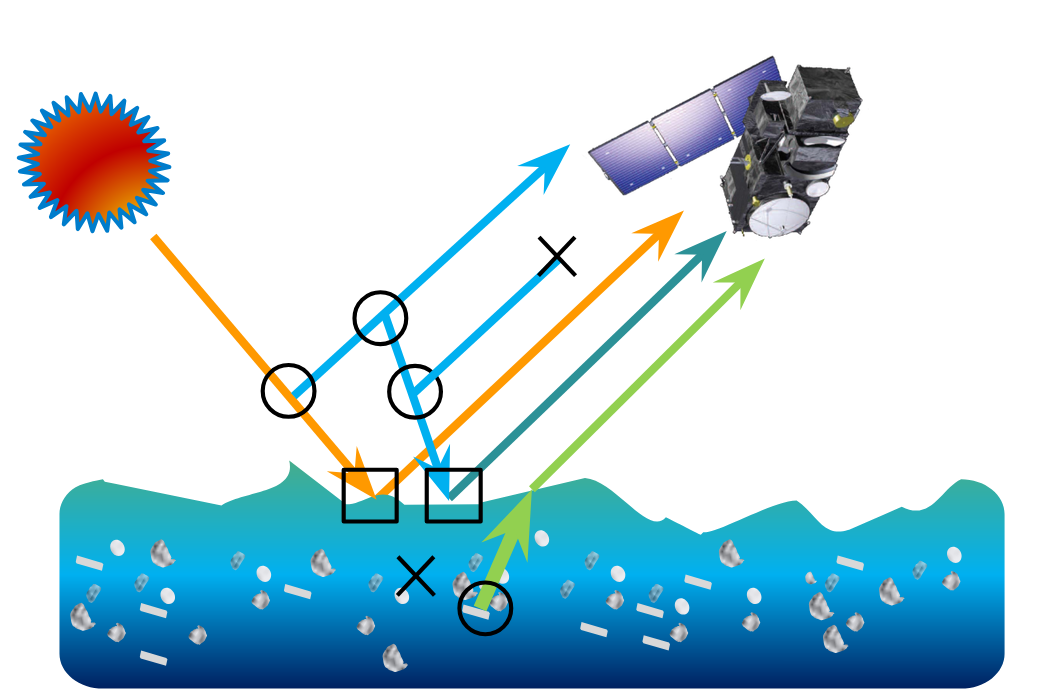
\includegraphics[width=0.43\textwidth]{visnir_radiation.png}} 
\subfigure(b){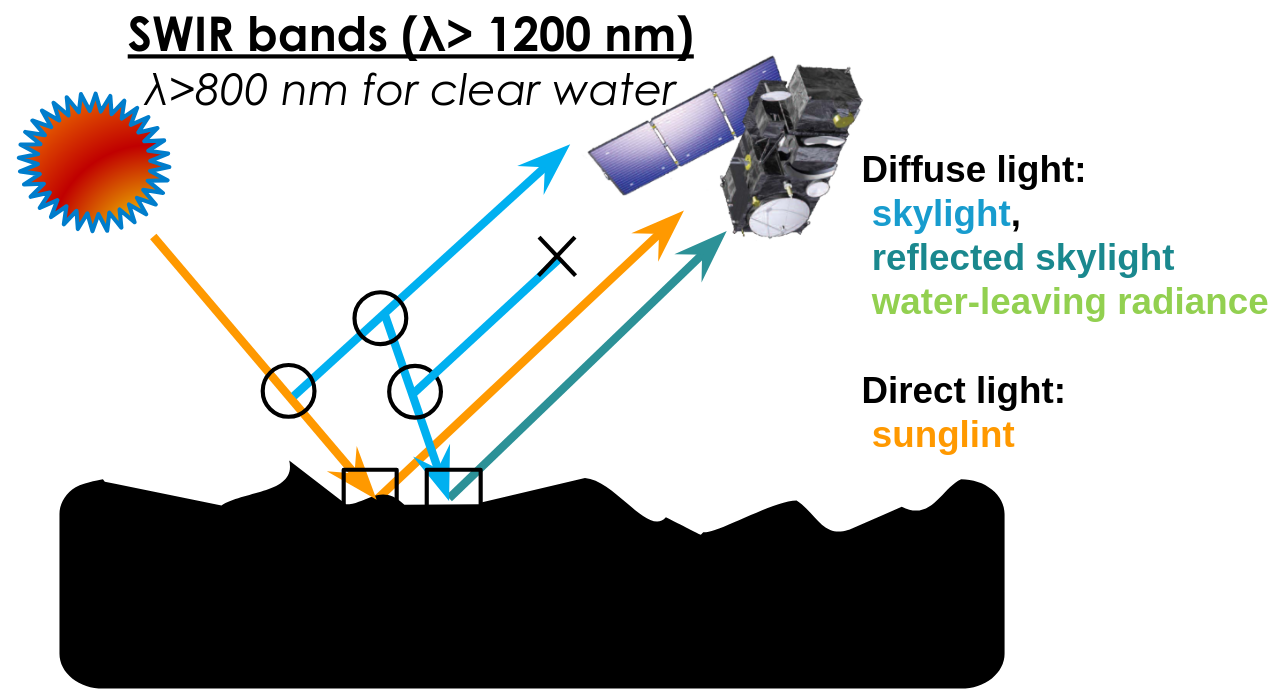
\includegraphics[width=0.53\textwidth]{swir_radiation.png}} 
\caption{Active components of light radiation at the top of the atmosphere in (a) the visible and near-infrared and (b) shortwave-infrared part of the spectrum. Scattering is depicted by circles whereas Fresnel reflection and absorption are depicted by squares and crosses, respectively.}
\label{fig:image2}
\end{figure}

\section{Radiative transfer model}

\subsection{Concept of remote sensing reflectance}
The  reflectance of a material has been defined as a ratio of radiometric flux exiting over the one received by this material. Within turbid media such as the atmosphere or the water column, we can define the reflectance as a dimensionless value equal to the ratio of spectral upwelling to downwelling plane irradiances at a given vertical location $z$ within the medium, for a given wavelength $\lambda$, as follows: 
\begin{equation}
R(z, \lambda) \equiv \frac{E_u(z, \lambda)}{E_d(z, \lambda)} \, .
\label{eq:placeholder}
\end{equation}
Nevertheless, in remote sensing applications, the upwelling plane irradiance cannot be directly measured. Instead, at pixel level, the detector measures the upwelling radiance, $L_u$, which is a function of the viewing geometry with: $\theta_s$ the sun zenith angle, $\theta_v$, the viewing zenith angle, and $\Delta\varphi$ the relative azimuth between Sun and viewing direction, see Figure \ref{fig:geometry}. Note that two conventions are commonly used for the latter: ($i$)  the radiative transfer convention where $\Delta\varphi$ is equal to zero when Sun and sensor are in opposition, ($ii$) the remote sensing convention where $\Delta\varphi$ is equal to $180^\circ$ in this configuration where the sun reflection on water (\textit{sunglint}) is likely to be visible in the radiometric measurement. As a result, the so-called remote sensing reflectance, $R_{rs}$, is dependent on the viewing geometry (\textit{i.e.}, anistropy of the upwelling radiance) and is expressed in unit of $sr^{-1}$, as follows:

\begin{equation}
R_{rs}(z=0^+, \lambda) = \frac{L_w(z=0^+,\theta_s,\theta_v,\Delta\phi, \lambda)}{E_d(z=0^+, \theta_s,\lambda)} \ \left(in\ sr^{-1}\right) .
\end{equation}
where $L_w$ is the water-leaving radiance (commonly expressed in  $mW\cdot m^{-2}\cdot sr^{-1}\cdot nm^{-1}$) and $E_d$ the downwelling plane irradiance (in $mW\cdot m^{-2}\cdot nm^{-1}$). Note that this parameter is defined just above the water surface ($z=0^+$) and therefore should be corrected for the contribution of the air-water interface reflection of sky and sunlight (and potentially from objects located on the surface: whitecaps, floating algae, etc.). Therefore, in remote sensing of the aquatic environment, the different algorithms should handle a proper retrieval and/or correction of the surface component of the signal from the measured upwelling radiance following the simple radiance decomposition:
\begin{equation}
L_{u}(z=0^+,\theta_s,\theta_v,\Delta\phi, \lambda) = L_w(z=0^+,\theta_s,\theta_v,\Delta\phi, \lambda) + L_{surf}(z=0^+,\theta_s,\theta_v,\Delta\phi, \lambda) .
\end{equation}
This is one of the main differences with remote sensing applications over land where the key reflectance to measure is \textit{simply} that at the bottom-of-atmosphere level. In this document, full modeling of the radiative transfer is detailed considering $R_{rs}$ and the other radiometric contributions within the coupled atmosphere-interface-water system to provide the theoretical basis of the \textit{atmospheric correction} algorithm of FLEX pixels.
\begin{figure}[h!]
    \centering
    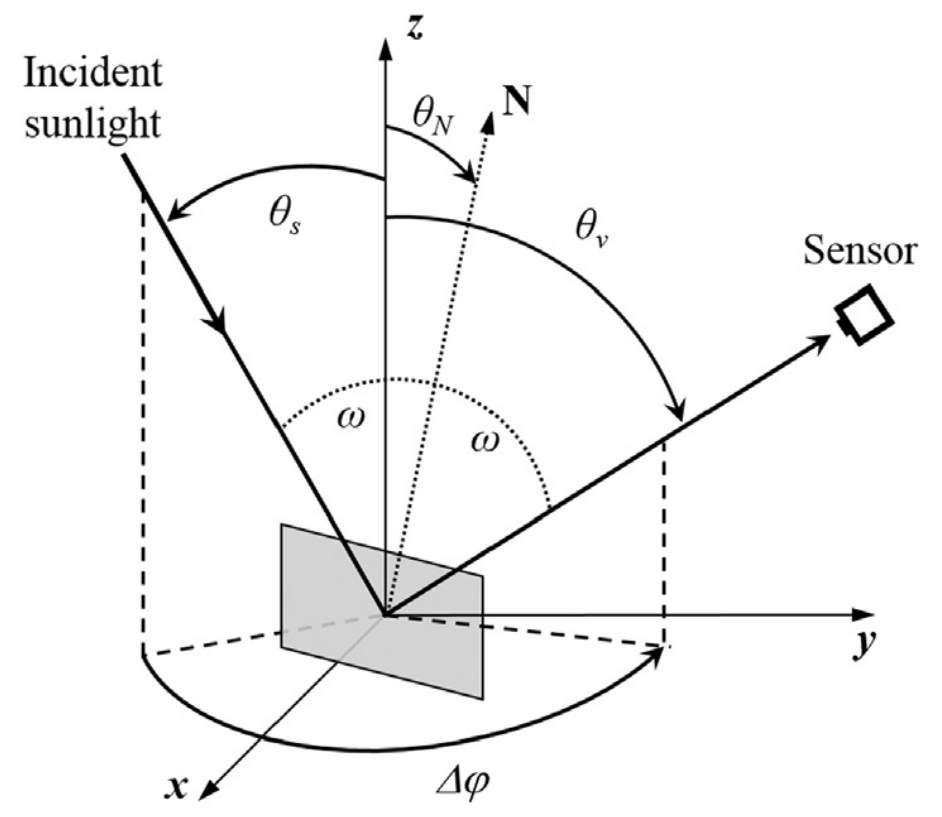
\includegraphics[width=0.5\linewidth]{sunglint_geometry.png}
    \caption{Coordinate system and definition of the relevant geometry parameters: $\theta_s$ and $\theta_v$
are the solar and the viewing zenith angles, respectively, $\Delta\varphi$ is the relative azimuth. The
vector N is the normal to the wave facet (gray area), $\theta_N$ is the angle of N with the vertical
and $\omega$ is the specular reflection angle.}
    \label{fig:geometry}
\end{figure}

\subsection{Radiative transfer equation and resolution}
Light taken as an electromagnetic radiation is fully described by its intensity and its polarization state. In order to provide convenient formalism to express the radiative transfer equation, the formalism of the Stokes vector has been adopted with the following definition:
\begin{equation}
\mathbf{S}=\left(I,Q,U,V\right)^T
\label{eq:stokes}
\end{equation}
where $I$ is the total intensity, $Q$ and $U$ express the linear polarization and $V$ the circular component of polarization. The term $I$ can easily be converted in radiance and therefore is the equivalent of the $L$ parameter described above. 
Above the oceans, the light radiation that exits the atmosphere originates from multiple interactions through the coupled system of the atmospheric and water layers, and their interface. Those interactions mainly depend on the absorption and scattering properties of the molecules and particulate matter in presence (\textit{e.g.}, gases, aerosols, hydrosols). Another important interaction to account for is the light reflection onto and the transmission through the rough air-water interface. Considering accurate modeling of the physical values attached to these interactions, the radiative transfer equation (RTE) may be solved to derive the light radiation reaching the satellite sensor for different scenarios (\textit{e.g.}, changing atmosphere or ocean constituents). The general form of the RTE can be expressed within a continuous medium as follows:
\begin{equation}
\mu \frac{d\mathbf{S}\left( \tau ,\mu ,\phi  \right)}{d\tau }=-\mathbf{S}\left( \tau ,\mu ,\phi  \right)+\frac{{{\omega }_{0}}\left( \tau  \right)}{4\pi }\int\limits_{0}^{2\pi }{d{\phi }'}\int\limits_{-1}^{1}{d{\mu }'}\mathbf{P}\left( \tau ,\mu ,\phi ,{\mu }',{\phi }' \right)\mathbf{S}\left( \tau ,{\mu }',{\phi }' \right)
\label{eq:rt_equation}
\end{equation}
where \textit{$\tau$} is the optical thickness along the vertical of the medium, $\mu$ and $\phi$ are the cosine of the viewing angle and the azimuth angle, respectively. The second term on the right-hand side of the equation, called the source term, depends explicitly on the phase matrix \textbf{P} and the single scattering albedo \textit{$\omega$\textsubscript{0}}. In the hydrologic optics nomenclature, \textit{$\omega$\textsubscript{0}} can be written as the ratio of \textit{b} aver \textit{c} where \textit{b} (m\textsuperscript{-1}) and \textit{c} (m\textsuperscript{-1}) are the scattering and attenuation coefficients, respectively. Here, it is preferred to express this albedo following the atmospheric optics nomenclature using the cross sections of absorption, $C_{abs}$, scattering, $C_{scat}$, and extinction (or \textit{attenuation}), $C_{ext}$. Those cross sections are expressed in $m^2$ and could be directly computed through single scattering numerical methods (\textit{e.g.}, Mie theory, T-matrix, discrete dipole approximation), see section \ref{aerosol}:
\begin{equation}
\label{ssa:equation}
{{\omega }_{0}}=\frac{{{C}_{sca}}}{{{C}_{ext}}}=\frac{{{C}_{sca}}}{{{C}_{abs}}+{{C}_{sca}}}
\end{equation}
In several applications of aquatic remote sensing, it can be useful to split the Stokes vector into its major components. For instance, at the sea surface level, the Stokes vector can be written as follows:
\begin{equation}
\label{stokes:equation}
\mathbf{S}_{\mathbf{tot}}^{{}}\mathbf{=}{{\mathbf{S}}_{\mathbf{atm}}}\mathbf{+}{{\mathbf{S}}_{\mathbf{sunglint}}}\mathbf{+}{{\mathbf{S}}_{\mathbf{surf}}}\mathbf{+S}_{\mathbf{w}}^{{}},
\end{equation}

where:
\begin{itemize}
    \item $\mathbf{S_{tot}}$ is the top-of-atmosphere Stokes vector that could be measured by the satellite sensor,
    \item $\mathbf{S_{atm}}$ is the contribution of the diffuse skylight of the atmosphere, note that here $\mathbf{S_{atm}}$ also contains reflection of the downwelling skylight on the air-water interface since the two are fully coupled,
    \item $\mathbf{S_{sunglint}}$ is the reflection of the direct sun light on the water surface, that is, light that underwent no scattering within the system but only reflection on the rough water surface,
    \item  $\mathbf{S_{surf}}$ is the contribution of floating material on the water surface (\textit{e.g.}, whitecaps, floating debris or algae), this parameter is neglected in the rest of this document,
    \item $\mathbf{S_{w}}$ stands for the Stokes vector water-leaving radiation. 
\end{itemize}


\subsection{Practical radiative transfer modeling}\label{sec:practical_rt}
The previous section described the proper resolution of the radiative transfer equation within our system. Nevertheless, resolution of the full radiative transfer within atmospheric correction procedure is practically intractable due to the heavy computing time required. The signal at the top of the atmosphere could opportunely be decomposed based on linear summation and use of \textit{ad hoc} transmittances, as follows: 
\begin{equation}
    L_{tot}^{TOA}(\lambda) = L_{atm}^{TOA}(\lambda) + L_{sunglint}^{TOA}(\lambda)+ L_{surf}^{TOA}(\lambda) + L_{w}^{TOA}(\lambda)
\label{eq:placeholder}
\end{equation}
\begin{equation}
    L_{tot}^{TOA}(\lambda) = L_{atm+surf}^{TOA}(\lambda) + T_{dir}(\theta_v)L_{sunglint}^{BOA}(\lambda) + T_g^{w}(\lambda)\,t_{L_u}(\theta_v)L_{w}^{BOA}(\lambda)
\label{eq:placeholder}
\end{equation}
which gives in reflectance unit:
\begin{equation}
    R_{tot}^{TOA} =\frac{L_{tot}^{TOA}}{E_o} = T_g^{atm} R_{atm+surf} + T_{dir}(\theta_v)T_{dir}({\theta_s})R_{sunglint}^{BOA} + T_g^{w}\,t_{L_u}(\theta_v)t_{E_d}(\theta_s)\pi R_{rs}^{BOA}
\label{eq:placeholder}
\end{equation}
with the following definitions:

\begin{itemize}
    \item \( R_{tot}^{TOA}\) and \(L_{tot}^{TOA}\)  the top-of-atmosphere reflectance and radiance, respectively, the final products to be compared with the satellite signal.
    \item \({E_o}\) is the extraterrestrial solar irradiance computed from the \textit{Total and Spectral Solar Irradiance Sensor-1 Hybrid Solar Reference Spectrum} (TSIS), v2 \cite{Coddington2023}.  TSIS solar reference spectrum is corrected for the variation of the Sun-Earth distance. A comparison between the different solar references is provided  Figure \href{}{\ref{fig:solar_ref}}.

    \item \(R_{atm+surf}\) : reflectance component of the atmosphere and sky reflection on the water surface, computed without gaseous absorption (look-up tables)
    \item \(R_{sunglint}^{BOA}\) : bottom-of-atmosphere reflectance of the sunglint (direct sunlight reflection on the water surface)
    \item \(R_{rs}^{BOA}\): remote sensing reflectance (water-leaving radiance divided by the downwelling irradiance)
    \item \(T_{dir}\):  direct transmittance, including the gaseous absorption of the direct beam,
    \[T_{dir}(\theta) = T_g(\lambda, 1/\cos\theta)\,\exp\left[-(\tau_r + \tau_a)/\cos\theta\right]\]
    \item \(T_g^{atm}\), \(T_g^{w}\): gaseous transmittances of the path reflectance and of the water-leaving term, coupled with the scattering (Section \ref{sec:coupling}); the downwelling irradiance at the surface is \(E_d = t_{E_d}(\theta_s)\,T_g^{E_d}\,E_0\)
    \item \(\theta_s\), \(\theta_v\): solar and viewing zenith angles, respectively
    \item \(t_{L_u}\): transmittance converting BOA to TOA upwelling radiance
    \item \(t_{E_d}\) : transmittance converting TOA to BOA downwelling irradiance
\end{itemize}
The gaseous absorption is not included in the look-up tables of the scattering (Section \ref{sec:lut}) and is applied
afterwards. In version 1.0 of this document, all the terms were given the transmittance of the direct beam, approximated
for the diffuse light by ad hoc scaling coefficients of the H$_2$O and O$_2$ optical thicknesses. Since version 1.1, each
term has its own transmittance, $T_g^{atm}$, $T_g^{w}$ and $T_g^{E_d}$, given by a photon path-length model of the absorption
coupled with the scattering (Section \ref{sec:coupling}).

\begin{figure}[h!]
\centering
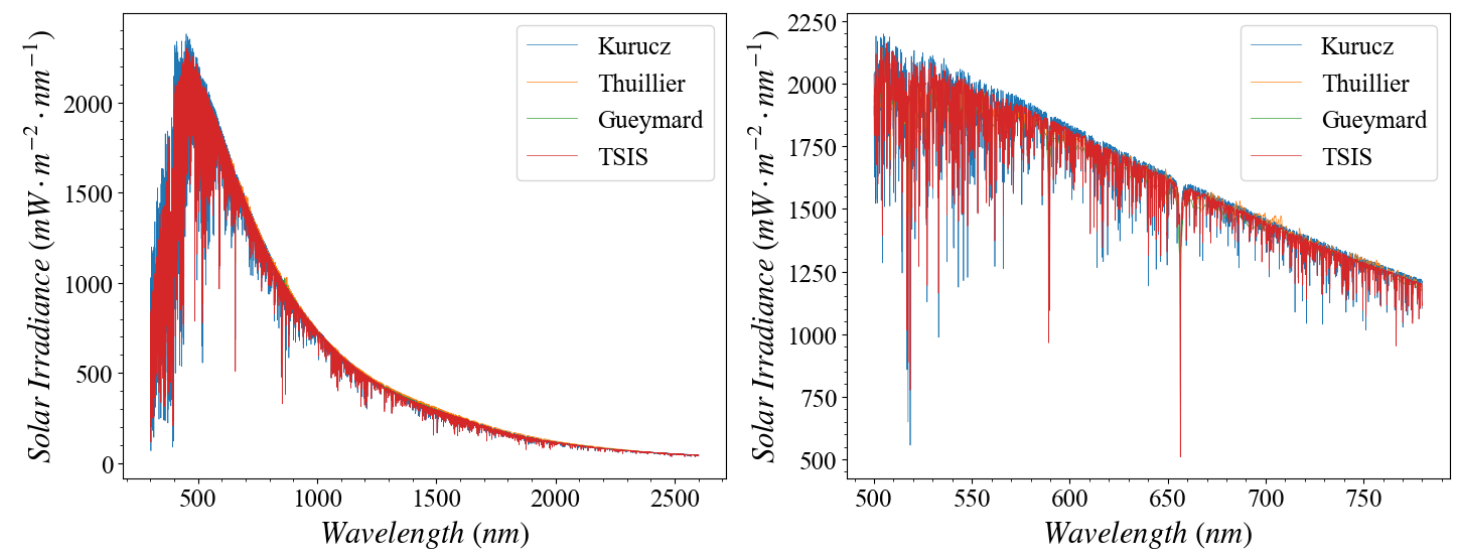
\includegraphics[width=.85\textwidth]{solar_reference.png}
\caption{Comparison between several solar irradiance references}
\label{fig:solar_ref}
\end{figure}

\subsection{Useful mathematical equations}
\subsubsection{Statistical averaging}
Due to the large number of particles in the atmospheric layers, it is convenient to model the aerosol properties based on the statistical distribution of their inherent microphysical properties such as size, shape, orientation, or refractive index. Here, the particles are assumed to be fully randomly oriented and the bulk refractive index is considered for a given aerosol type. In this condition, the probability function that describes the aerosols is based only on the distribution of the size and shape. For practical reasons, particle shapes and sizes are assumed statistically independent enabling to separate averaging over these two parameters:
\begin{equation}
P\left( \varepsilon ,r \right)=n\left( \varepsilon  \right)n\left( r \right)
\end{equation}                           	
Note that all the probability functions used in the following are normalized to unity.

\begin{equation}
\int\limits_{{{\varepsilon }_{\min }}}^{{{\varepsilon }_{\max }}}{n\left( \varepsilon  \right)d\varepsilon }=1,
\end{equation}

\begin{equation}     	
\int\limits_{{{r}_{\min }}}^{{{r}_{\max }}}{n\left( r \right)dr}=1,
\end{equation}
 
\subsubsection{Size distribution}
The size distribution of particles, denoted as $n$, is defined as the derivative of the total concentration number $N$ by the size of the particles. Assuming spherical particles, this size is directly given by the radius attached to each particle, and the size distribution can be written as follows:
\begin{equation}  
                              	n\left( r \right)=\frac{dN\left( r \right)}{dr}                                 	
\end{equation}
Many studies showed that the size distribution of most aerosols can be modeled as a lognormal distribution:
\begin{equation}  
\frac{dN\left( r \right)}{dr}=\frac{{{N}_{0}}}{\sigma _{n}^{{}}r\sqrt{2\pi }}\exp \left( -\frac{{{\left( \log \left( {r}/{{{r}_{nm}}}\; \right) \right)}^{2}}}{2\sigma _{n}^{2}} \right)                 	
\end{equation}
where $N_0$ is the total number of particles per unit of volume (here taken as unity for normalization purposes), $r_{nm}$ is the median radius of the distribution and ${{\sigma }_{n}}$ its standard deviation.
\begin{equation}  
\frac{dV\left( r \right)}{d\log r}=\frac{{{V}_{0}}}{\sigma _{v}^{{}}\sqrt{2\pi }}\exp \left( -\frac{{{\left( \log \left( {r}/{{{r}_{vm}}}\; \right) \right)}^{2}}}{2\sigma _{v}^{2}} \right),
\end{equation}
where $V$ is the volume density distribution and $r$ the radius of the particles; and $V_0$ the total particle volume per unit of volume (for normalization, $V_0=1\ µm^3\cdot  cm^{-3}$ in the following).
For the sake of brevity, let us now define ${{\mu }_{n}}=\log {{r}_{nm}}$ and ${{\mu }_{v}}=\log {{r}_{vm}}$ . In the case of the lognormal distribution it is easy to show that (see \cite{Grainger2012} for details):
\begin{equation}  
                            {{\mu }_{n}}={{\mu }_{v}}-3{{\sigma }^{2}},
\end{equation}                            	
with
\begin{equation}  
                             	\sigma ={{\sigma }_{n}}={{\sigma }_{v}}.
\end{equation}
Note that the transformation needed to keep the unity normalization between number and volume distribution:
   \[{{V}_{0}}=\frac{4\pi }{3}\exp \left( 3{{\mu }_{n}}+4.5{{\sigma }^{2}} \right)\]  	
a multimodal lognormal size distribution assuming spherical particles, as follows:
\[\frac{dV\left( r \right)}{d\log r}=\frac{{{V}_{0}}}{\sqrt{2\pi }}\sum\limits_{i}^{{{N}_{\bmod }}}{\frac{{{\beta }_{i}}}{\sigma _{v,i}^{{}}}}\exp \left( -\frac{{{\left( \log \left( {r}/{{{r}_{vm,i}}}\; \right) \right)}^{2}}}{2\sigma _{v,i}^{2}} \right),\]                                                              	
The terms ${{r}_{vm,i}}$, ${{\sigma }_{v,i}}$ and ${{\beta }_{i}}$ are the median radius for the volume distribution, the standard deviation, and the volumetric proportion of the lognormal mode $i$, respectively.

\subsubsection{Shape distribution}
 Similarly to the size distribution and following Kandler et al. \citeyear{Kandler2007}, the probability density function of aerosol shapes can be expressed through a lognormal distribution of the parameter ($\varepsilon-1$).
                                                        	\begin{equation}   
                                                            \begin{split}
   n\left( \varepsilon  \right)&=\frac{dN}{d\varepsilon } \\
  &=\frac{1}{\sqrt{2\pi }{{\sigma }_{\varepsilon }}\left( \varepsilon -1 \right)}\exp \left( -\frac{{{\left( \log \left( \varepsilon -1 \right)-\log \left( {{\varepsilon }_{m}}-1 \right) \right)}^{2}}}{2\sigma _{\varepsilon }^{2}} \right) 
\end{split}
\end{equation}



\subsection{Aerosol optical properties} \label{aerosol}

In atmospheric correction the retrieval of the spectral component of the aerosol (atmosphere signal) is of paramount importance both for the diffuse light correction with associated diffuse transmission of the atmosphere and for the computation of the sunglint signal (direct sunlight reflected toward the sensor).

The scattering matrix describes the interaction between the incident beam with molecules and the suspended matter within a sample. The Mueller scattering matrix \textbf{$\mathbf{F}$} is defined based on the Stokes vector formalism, as the matrix that transforms an incident Stokes vector $\mathbf{S}$ into the scattered Stokes vector $\mathbf{S'}$ as:
\begin{equation}   
\mathbf{S'} = \begin{pmatrix} I' \\ Q' \\ U' \\ V' \end{pmatrix} \\ 
= \dfrac{C_{\text{sca}}}{4 \pi r^2} \mathbf{F S} = \begin{pmatrix} F_{11} & F_{12} & F_{13} & F_{14} \\ F_{21} & F_{22} & F_{23} & F_{24} \\ F_{31} & F_{32} & F_{33} & F_{34} \\ F_{41} & F_{42} & F_{43} & F_{44} \end{pmatrix} \begin{pmatrix} I \\ Q \\ U \\ V \end{pmatrix}.
\label{eq:general_scatmat}

\end{equation}

Note that the first term of $\mathbf{S'}$, that is, $I’$ corresponds to the radiance or the radiance reflectance depending on the unit definition. The above scattering matrix is defined with respect to the scattering plane (i.e., the plane through the incident and scattered beams). In general, the scattering matrix of aerosols (or hydrosols) can be simplified and expressed for a given scattering angle $\Theta$ as follows:
\begin{equation}   
\mathbf{F}(\Theta)=\begin{pmatrix}\!F_{11}(\Theta) & F_{12}(\Theta) & 0 & 0\\F_{12}(\Theta) & F_{22}(\Theta) & 0 & 0\\0 & 0 & F_{33}(\Theta) & F_{34}(\Theta)\\0 & 0 & -F_{34}(\Theta) & F_{44}(\Theta)\end{pmatrix}
\label{eq:scat_mat}
\end{equation}
Note that the phase matrix $\mathbf{P}$ is obtained by rotating this matrix $\mathbf{F}$ to the reference plane (usually the meridian plane) that produces non-null diagonal terms in $\mathbf{P}$, see \cite{Mishchenko2000a} for details.

\subsubsection{Aerosol models from OPAC database}
Aerosol models are built on the OPAC database \cite{Hess1998} that includes spectral complex refractive index, size distribution, hygroscopicity changes and non-spherical particles. The hygroscopic growth is modeled as follows:
\begin{equation}
    r_{wet} = r_{dry}\left(1+\kappa\frac{RH}{1-RH}\right)^{1/3}
\label{eq:hygroscopy}
\end{equation}
where $r_{wet}$ is the radius used in \textit{single scattering} computation and $r_{dry}$ the median radius as listed in table \ref{tab:opac_component}. Another key parameter is the refractive index of each aerosol component with the spectral complex refractive index, taking the following notation:
\begin{equation}
    m\left(\lambda\right) =  m_r\left(\lambda\right)+ im_i\left(\lambda\right)
\label{eq:refrac_index}
\end{equation}
The spectrally dependent values were taken from tabulated values from the literature as shown in Figure \ref{fig:refrac_index}. The Optical Properties of Aerosol and Clouds (OPAC) aerosol models are generated based on a mixture of pure components that are listed in table \ref{tab:opac_component}. These components are representative of the main aerosol properties retrieved on a global scale. One advantage of those models is to consider the spectral variation of the complex refractive index and non-spherical shapes of the individual aerosols.
\begin{figure}[htbp!]
    \centering
    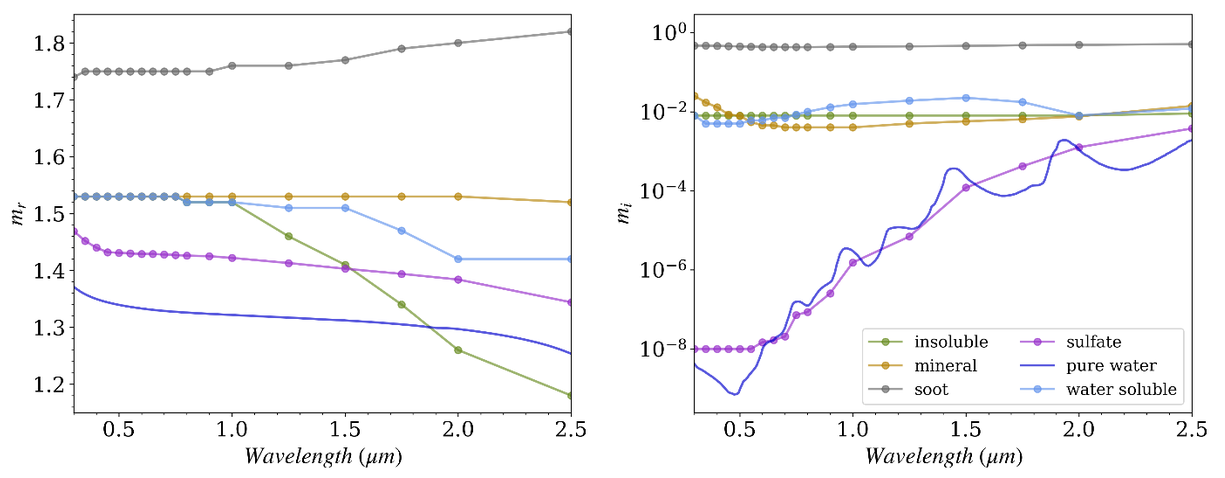
\includegraphics[width=0.85\linewidth]{refrac_index_aerosol.png}
    \caption{Spectral variation of the (left) real part and (right) imaginary part (driving the absorption properties) of the complex refractive index of the OPAC aerosol components.}
    \label{fig:refrac_index}
\end{figure}



\begin{table}[htbp] 
\centering 

\caption{Description of the microphysical parameters of the OPAC components for aerosol modeling.}
\small
\begin{tabular}{lllllllllll}
\hline
Component & name & sigma & rmed\_N & rmed\_V & rmin & rmax & density & shape & kappa & refrac\_index \\
\hline
Insoluble & INSO & 2.51 & 0.471 & 6 & 0.005 & 20 & 2 & sphere & 0 & insoluble \\
\hline
Water-soluble & WASO & 2.24 & 0.0212 & 0.15 & 0.005 & 20 & 1.8 & sphere & 0.27 & water\_soluble \\
\hline
Soot & SOOT & 2 & 0.0118 & 0.05 & 0.005 & 20 & 1 & sphere & 0 & soot \\
\hline
Sea salt

(acc.mode) & SSAM & 2.03 & 0.209 & 0.94 & 0.005 & 20 & 2.2 & spheroid & 1.12 & seasalt \\
\hline
Sea salt 

(coa. mode) & SSCM & 2.03 & 1.75 & 7.9 & 0.005 & 60 & 2.2 & spheroid & 1.12 & seasalt \\
\hline
Mineral

(nuc. mode) & MINM & 1.95 & 0.07 & 0.27 & 0.005 & 20 & 2.6 & spheroid & 0.1 & mineral \\
\hline
Mineral

(acc. mode) & MIAM & 2 & 0.39 & 1.6 & 0.005 & 20 & 2.6 & spheroid & 0.1 & mineral \\
\hline
Mineral

(coa. mode) & MICM & 2.15 & 1.9 & 11 & 0.005 & 60 & 2.6 & spheroid & 0.1 & mineral \\
\hline
Mineral-transported & MITR & 2.2 & 0.5 & 3 & 0.02 & 5 & 2.5 & spheroid & 0.05 & mineral \\
\hline
Sulfate droplets & SUSO & 2.03 & 0.0695 & 0.31 & 0.005 & 20 & 1.7 & sphere & 0.53 & sulfate \\
\hline

\end{tabular}

    \label{tab:opac_component}
\end{table}

\begin{table}[htbp] 
\caption{Mixture in aerosol components defining the different aerosol models used to generate look-up tables.}
\centering
\small
\begin{tabular}{l l l l l l l l l l l l}
\hline
name & Aerosol types & INSO & WASO & SOOT & SSAM & SSCM & MINM & MIAM & MICM & MITR & SUSO \\
COAV & Continental averaged & 0.4 & 7000 & 8300 & 0 & 0 & 0 & 0 & 0 & 0 & 0 \\
URBA & Urban & 1.5 & 28000 & 130000 & 0 & 0 & 0 & 0 & 0 & 0 & 0 \\
DESE & Desert & 0 & 2000 & 0 & 0 & 0 & 269.5 & 30.5 & 0.142 & 0 & 0 \\
MACL & Maritime clean & 0 & 1500 & 0 & 20 & 3.20E-03 & 0 & 0 & 0 & 0 & 0 \\
ARCT & Arctic & 0.01 & 1300 & 5300 & 1.9 & 0 & 0 & 0 & 0 & 0 & 0 \\

\end{tabular}
    \label{tab:opac_model}
\end{table}

\subsubsection{Spectral extinction and absorption}

The extinction cross-sections and the single scattering albedo are shown spectrally in Figure \ref{fig:cext_opac} for the OPAC models generated based on the microphysical parameters listed in tables \ref{tab:opac_component} and \ref{tab:opac_model}. Note the different spectral behaviors of the aerosol models and the specific feature of the single scattering albedo driven by the absorption characteristics of the aerosol components over the range from the visible to NIR. The consideration of the full spectral properties is crucial for the accurate handling of the sunglint signal, for instance. 

\begin{figure}[H]
    \centering
    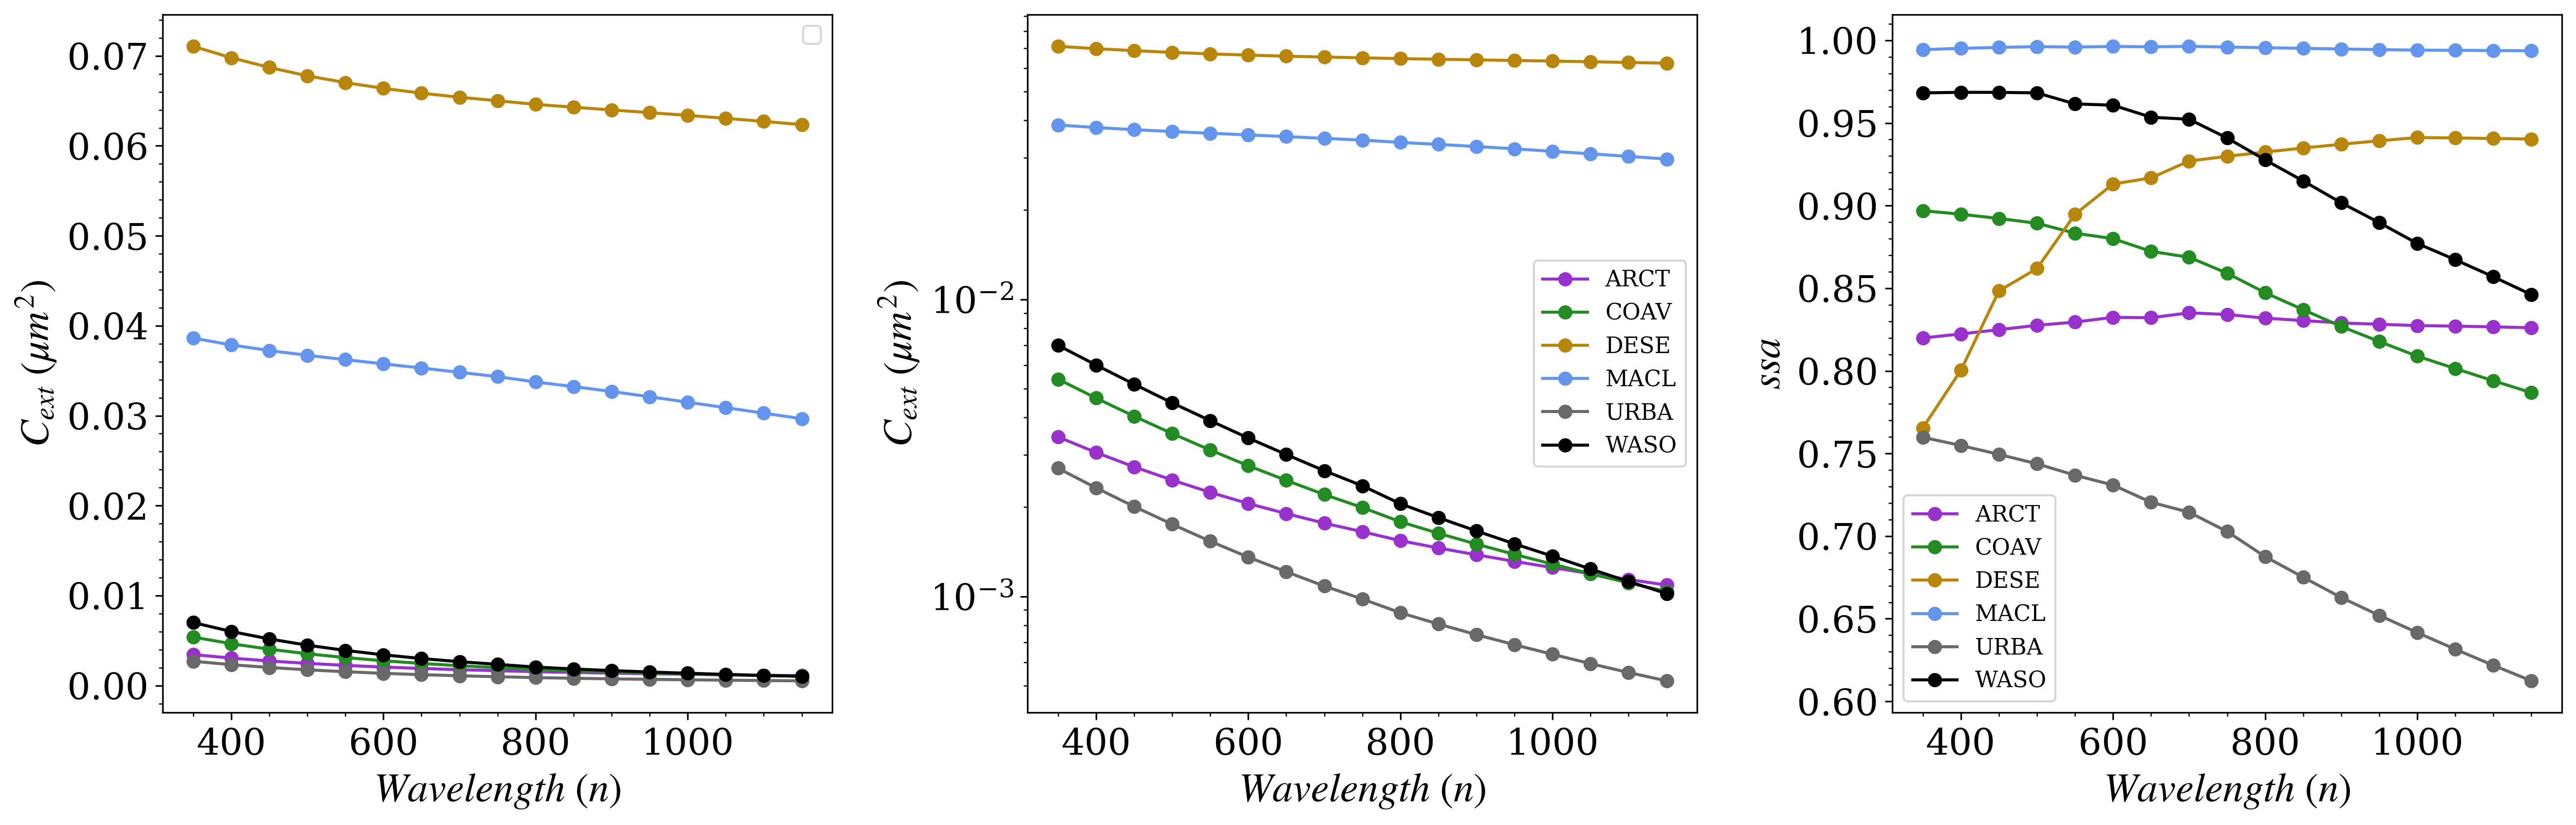
\includegraphics[width=1\linewidth]{spectral_prop_aerosol_OPAC.png}
    \caption{Spectral extinction cross sections and single scattering albedos of the OPAC aerosol models implemented in the atmospheric correction}
    \label{fig:cext_opac}
\end{figure}

\subsubsection{Scattering matrix}
In radiative transfer computations, the full scattering matrix has to be considered even for the intensity (or radiance) computation due to the non-diagonal terms introduced in equations  \ref{eq:general_scatmat} and \ref{eq:scat_mat}. Here, the microphysical parameters of table \ref{tab:opac_component} were used to generate the scattering matrix based on \textit{Mie} theory for homogeneous sphere, \textit{T-matrix} for ellipsoidal/spheroidal particles; these computations were extended for large particle sizes with the “\textit{Improved Geometric Optics Method}” \cite{Yang2007}. The computations were performed through the MOPSMAP package (\textit{Modeled optical properties of ensembles of aerosol particles}) coded in FORTRAN and based on pre-computed look-up tables \cite{Gasteiger2018}.  Note that, unlike spherical aerosol models, the scattering matrices exhibit $F_{22}$ that departs from the equality with $F_{11}$ with an impact on the computation of the top-of-atmosphere radiance. The following figures show the variation of the terms of the scattering matrices of the implemented aerosol models for wavelengths in the green, NIR (500, 800 nm, respectively).
\begin{figure}[H]
    \centering
    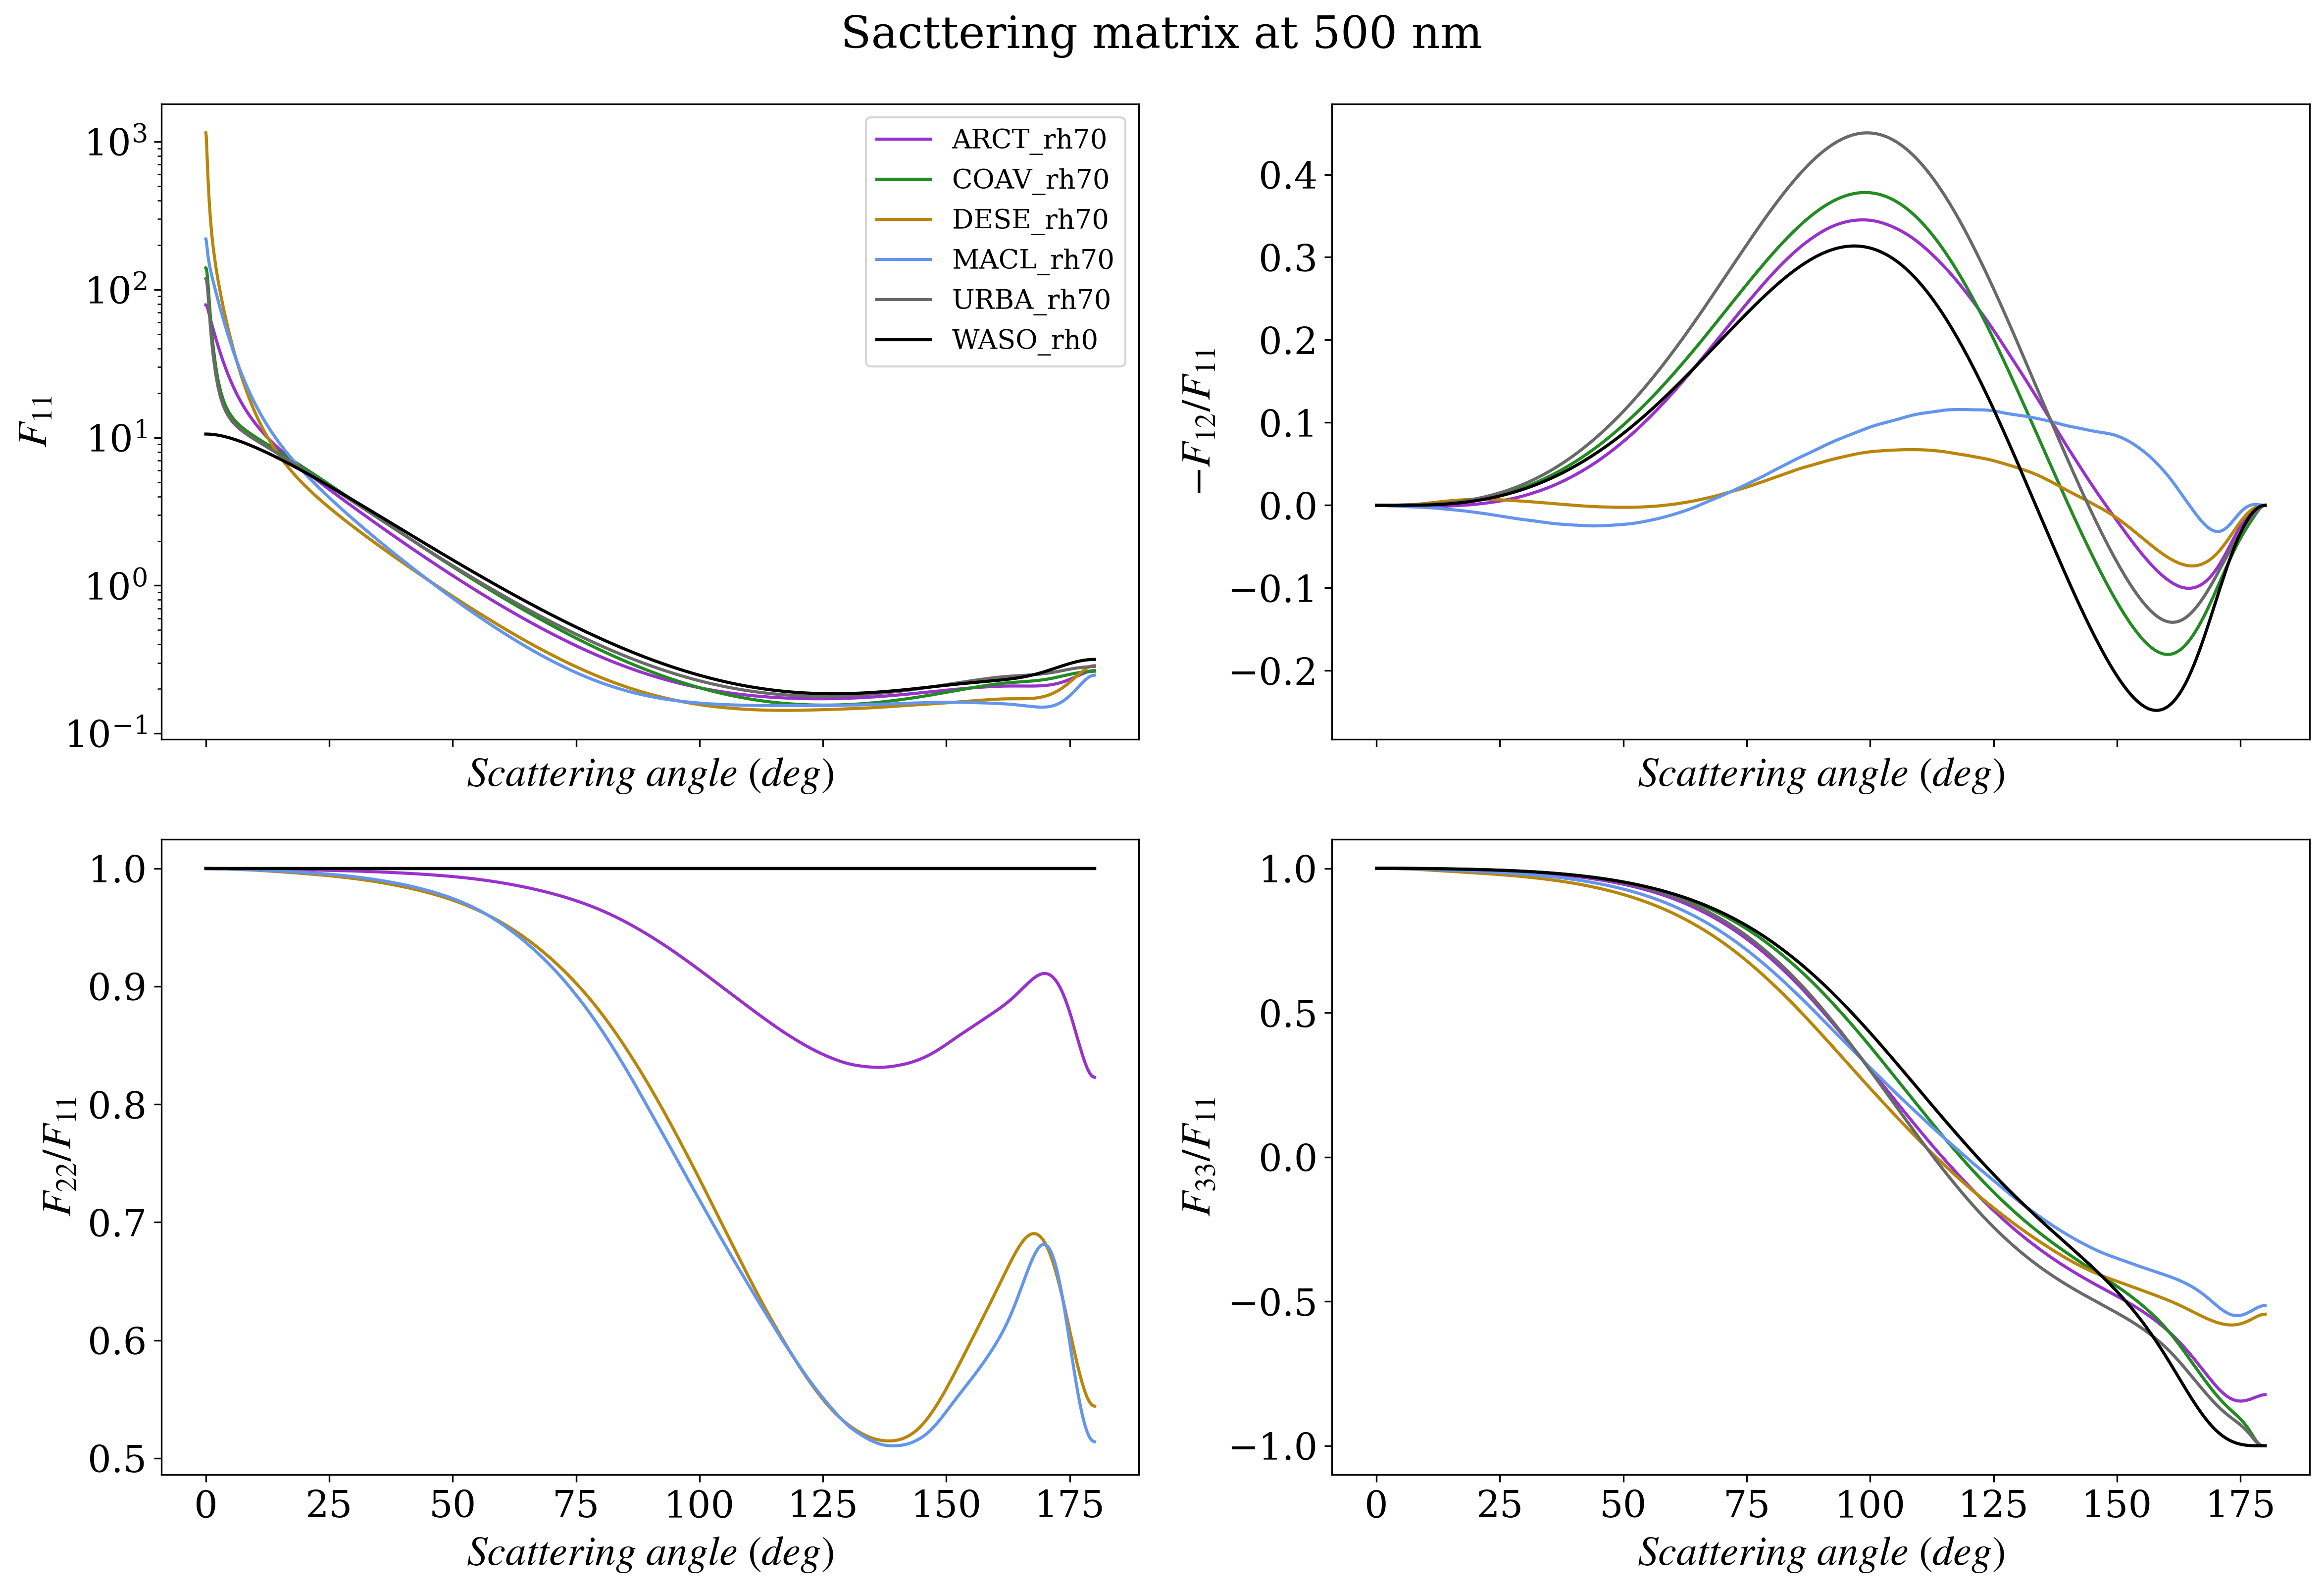
\includegraphics[width=0.8\linewidth]{scatt_mat_aerosol_OPAC_500nm.png}
    \caption{Non-null terms of the scattering matrix at 500 nm of the OPAC models implemented in this study.}
    \label{fig:scat_mat_500nm}
\end{figure}
\begin{figure}[h!]
    \centering
    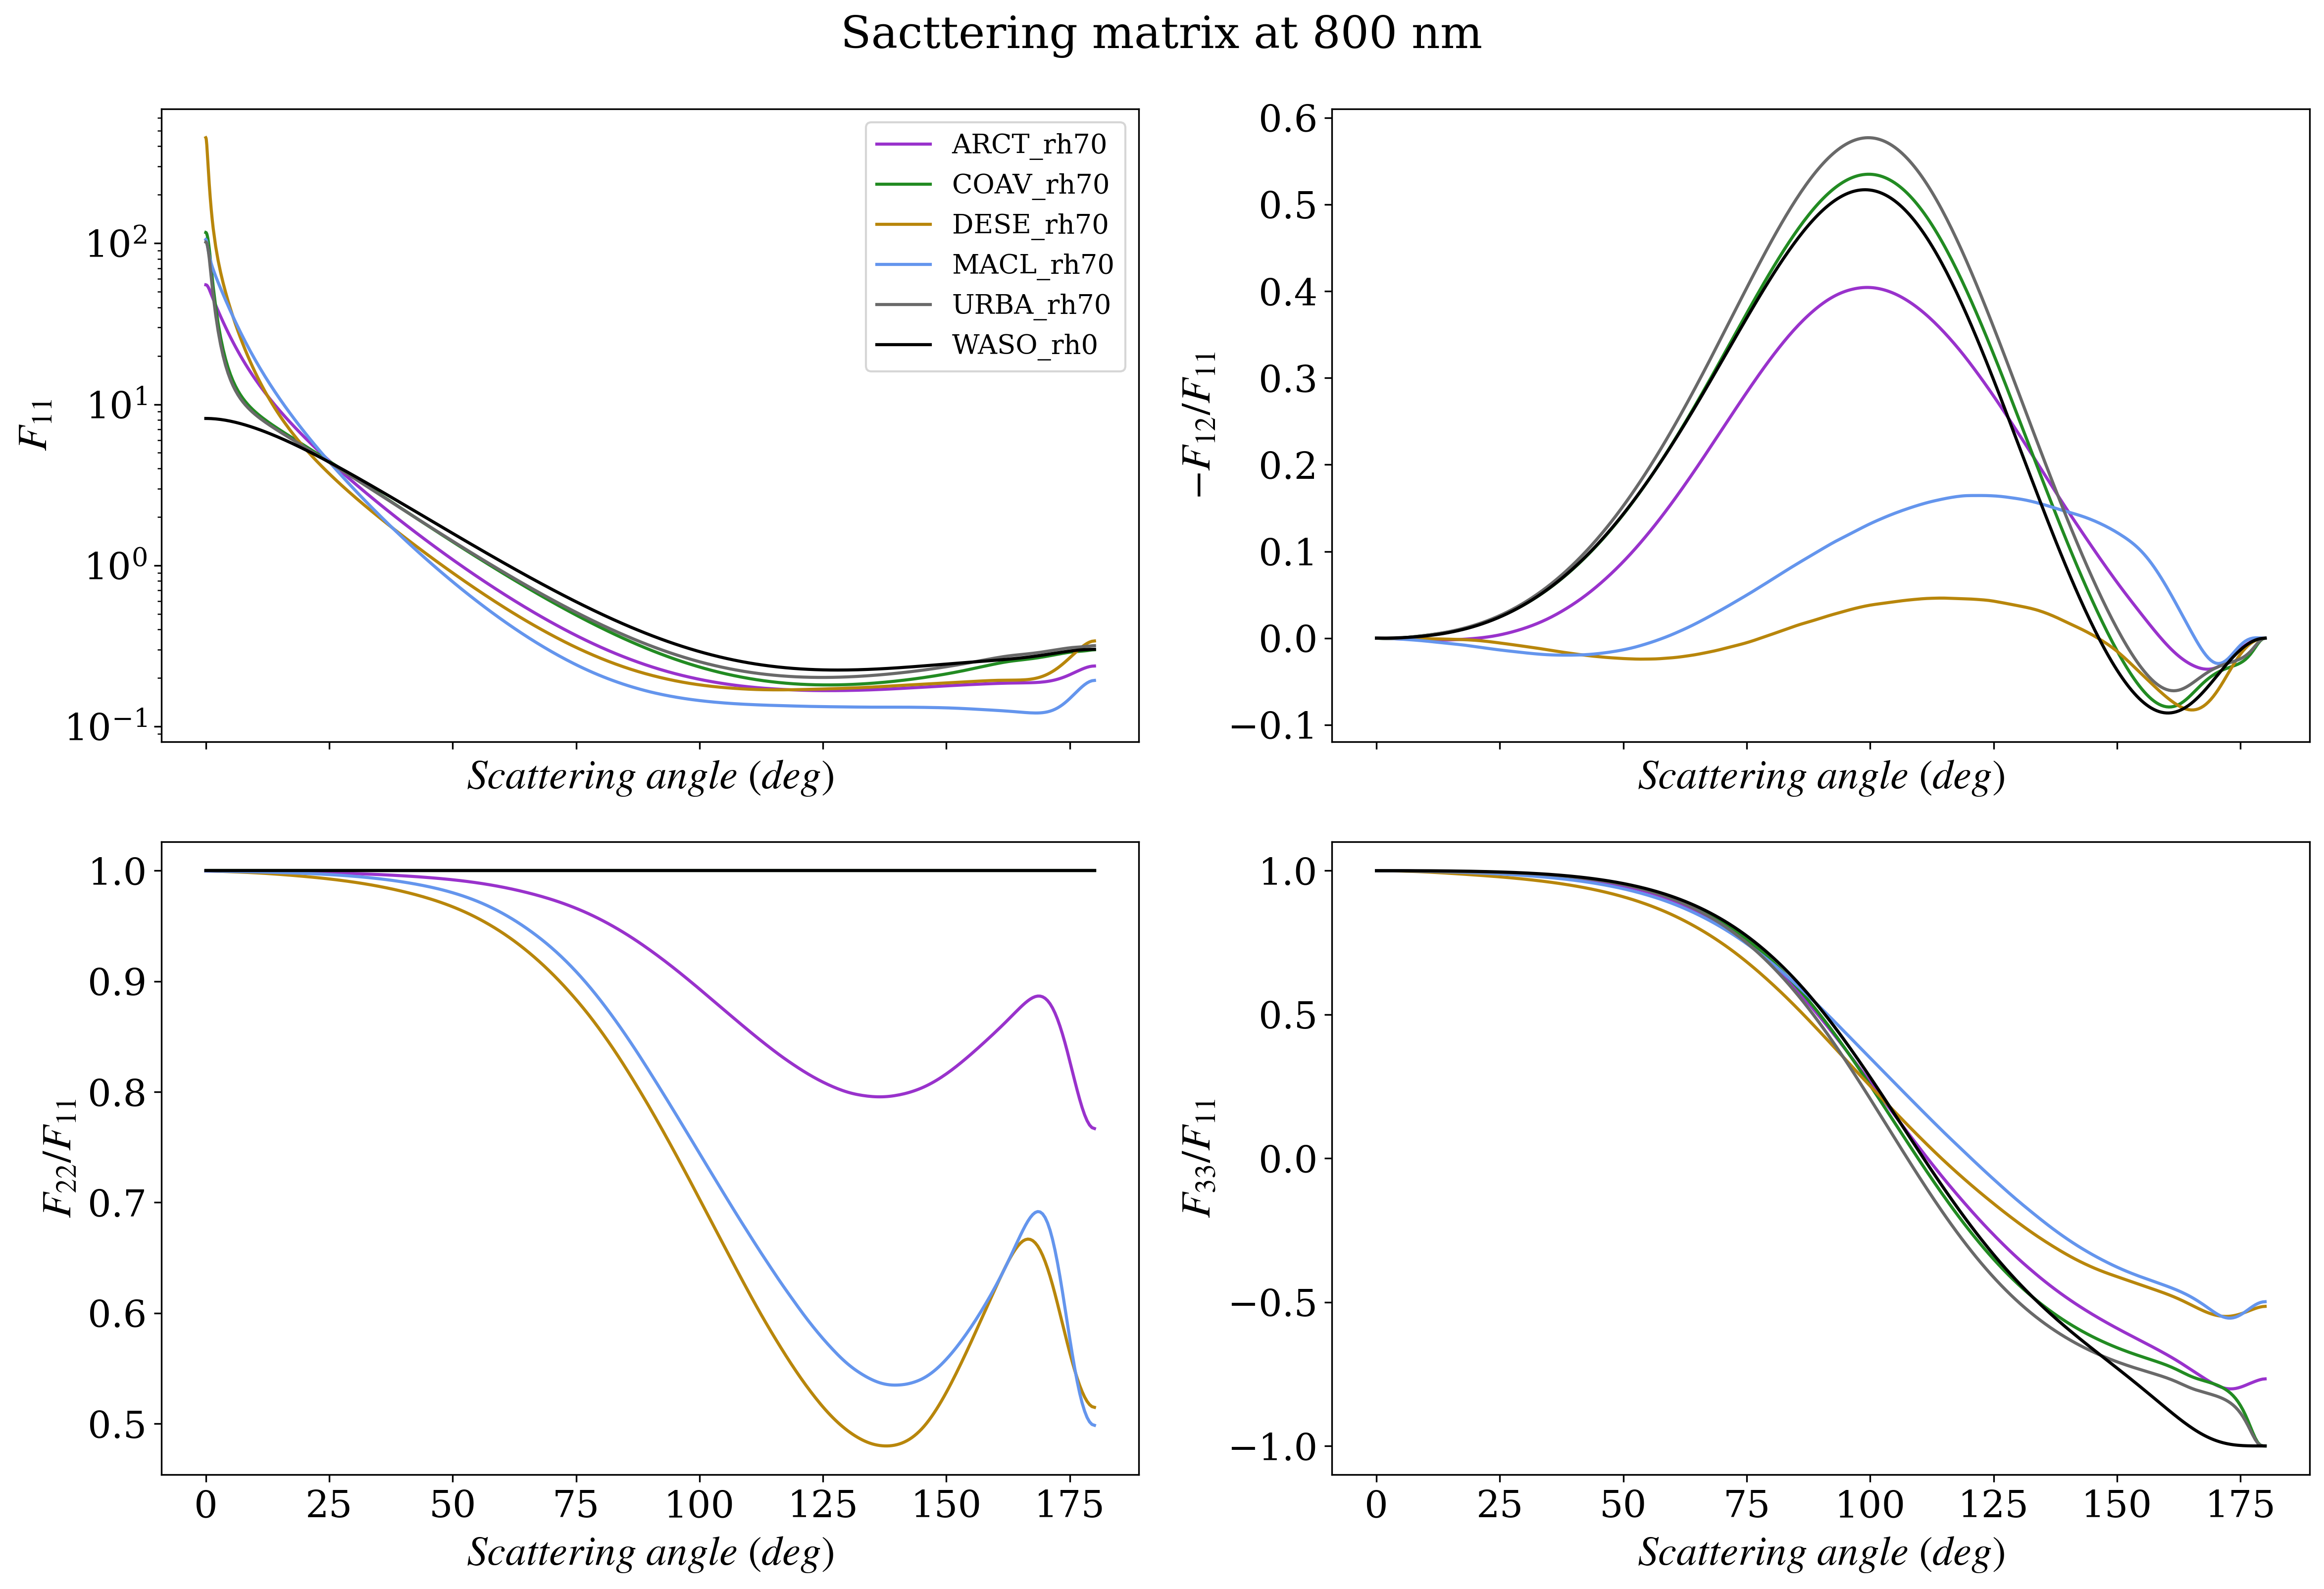
\includegraphics[width=0.8\linewidth]{scatt_mat_aerosol_OPAC_800nm.png}
    \caption{Non-null terms of the scattering matrix at 800 nm of the OPAC models implemented in this study.}
    \label{fig:scat_mat_800nm}
\end{figure}

\subsection{Gaseous absorption}
Different major elements were accounted for in the computation of the optical properties of absorbing gases with: $H_2O$ (water vapor), $O_2$, $O_3$, $O_4$ , $CH_4$, $CO_2$, $N_2O$  as illustrated in Figure \ref{fig:abs_trans_elements}. The optical thicknesses were scaled for an integrated columnar value of  1 $kg\cdot m^{-2}$ for each element from the LibRadTran library. The following figures \ref{fig:abs_trans_elements} and \ref{fig:computed_trans} show the different spectral behaviors of the absorbing molecules and the total transmittance, respectively.

\begin{figure}[H]
    \centering
    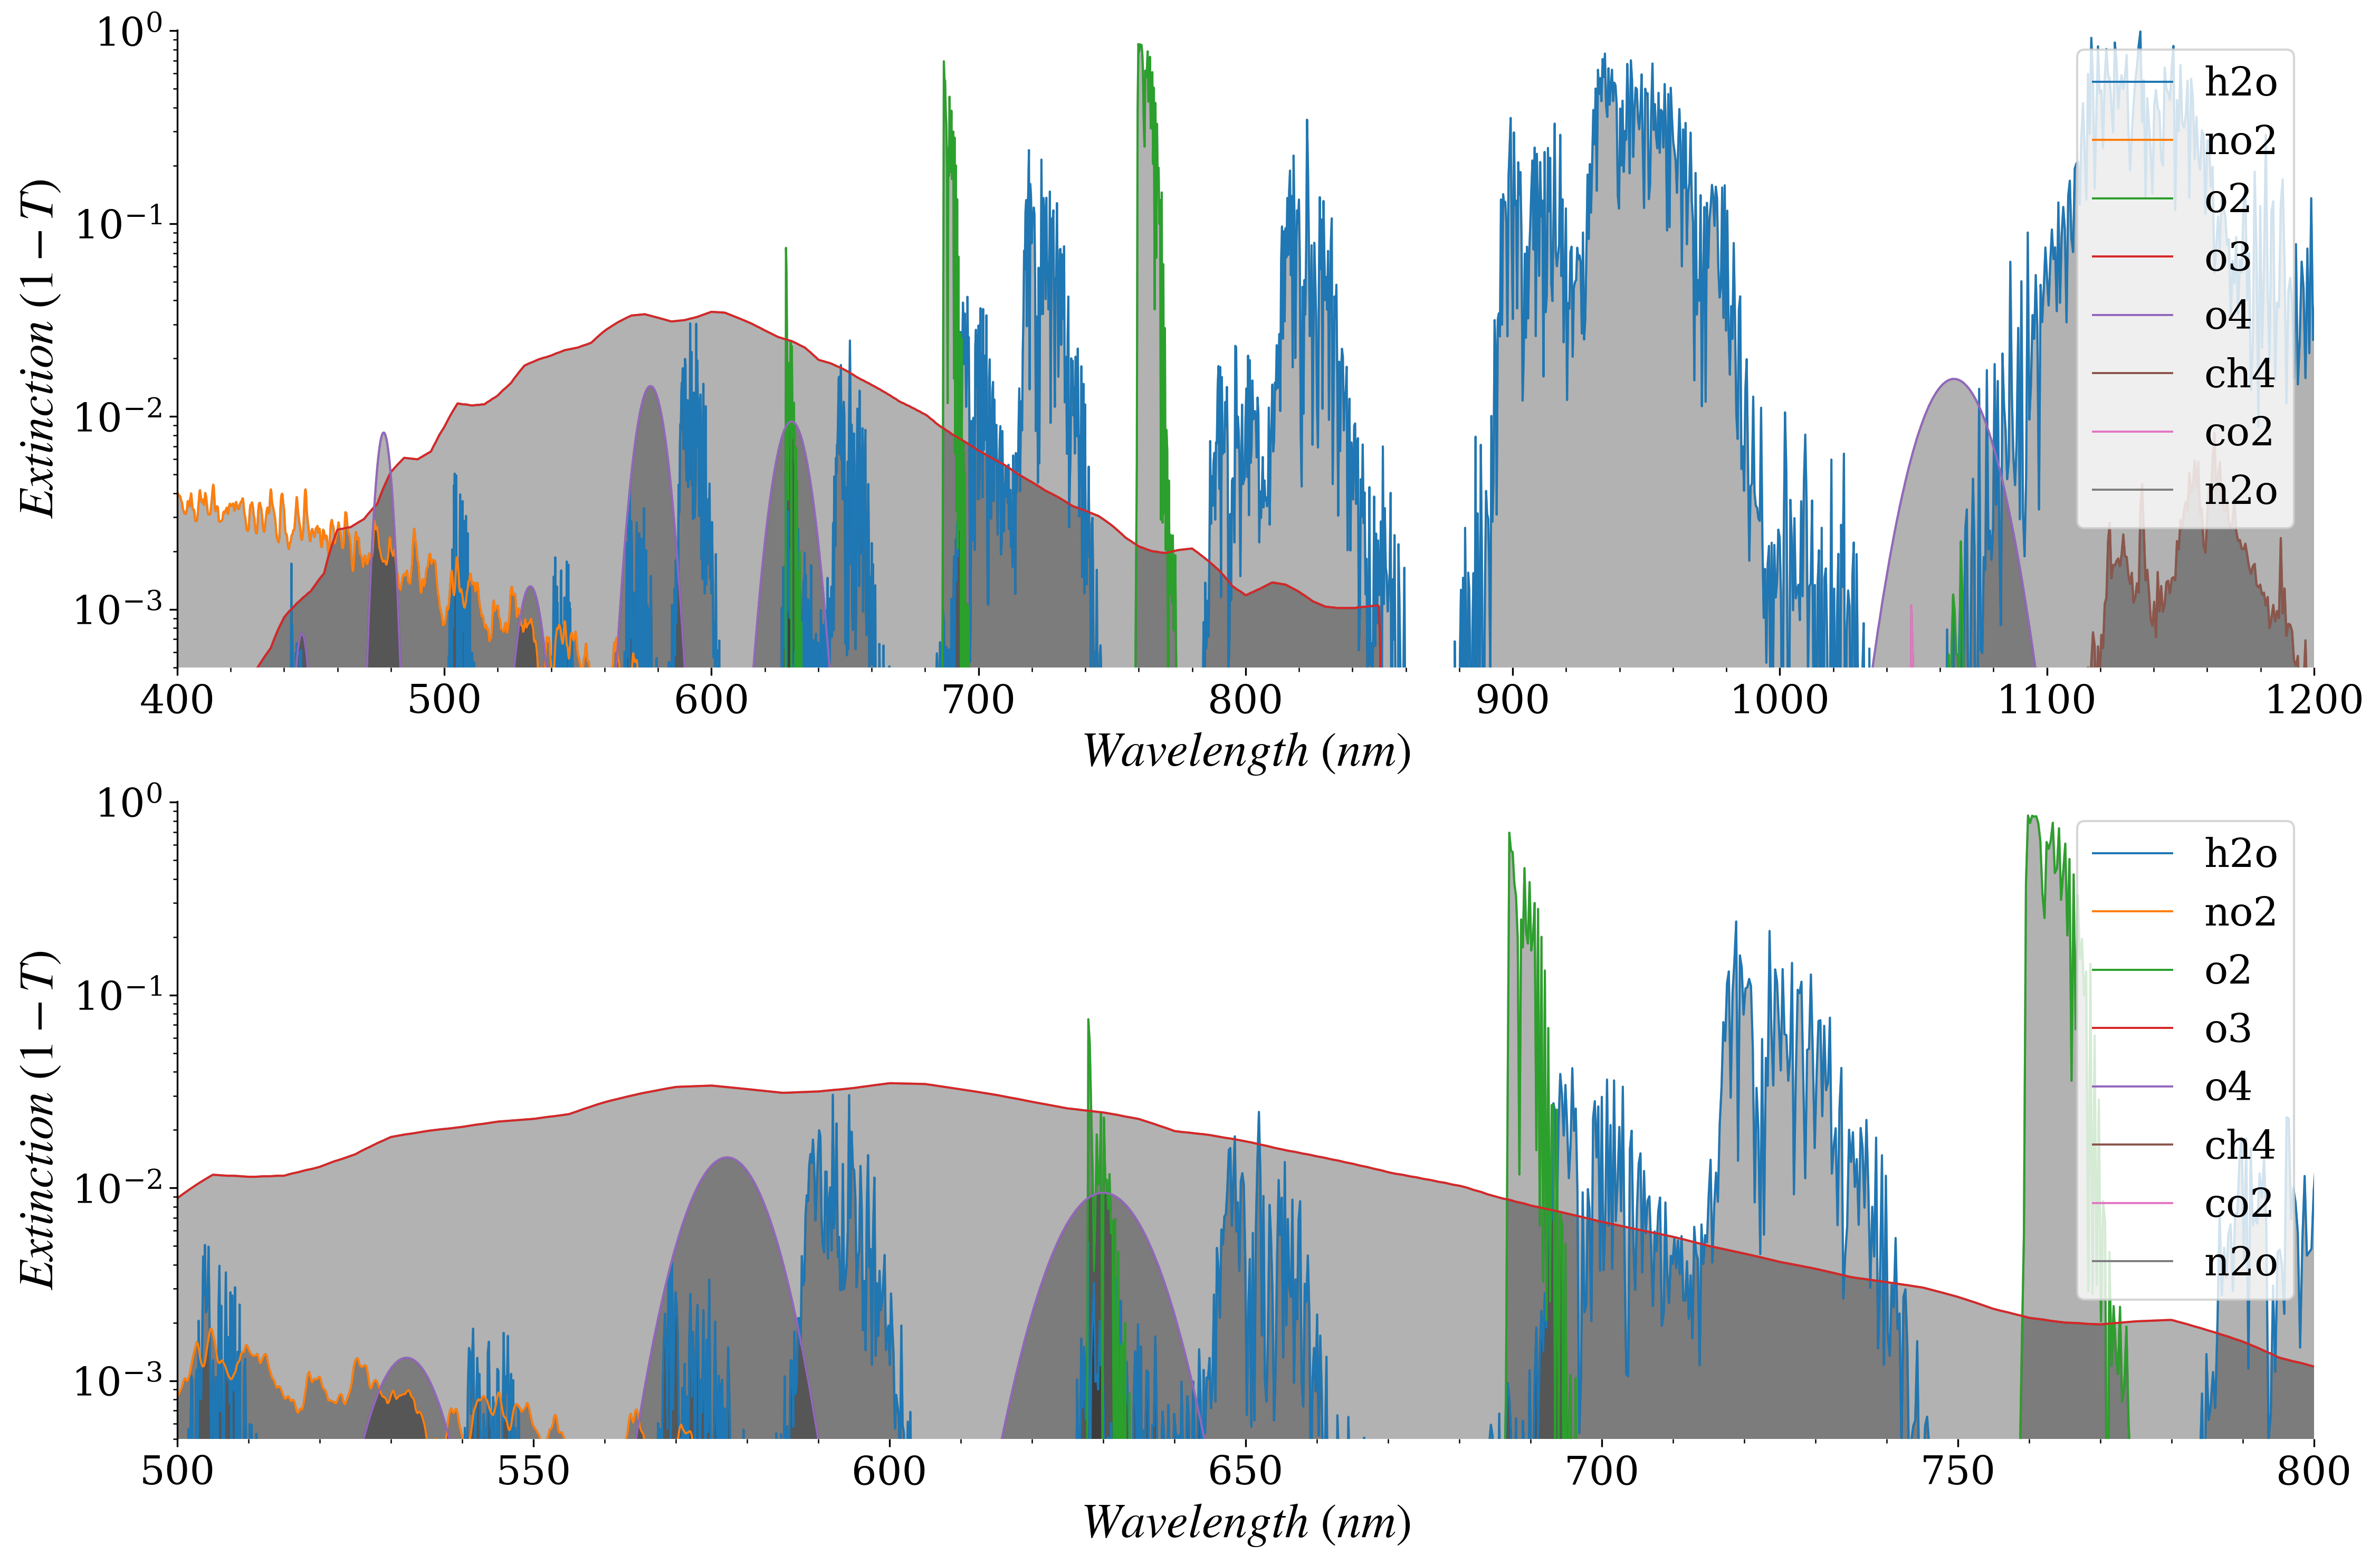
\includegraphics[width=0.8\linewidth]{abs_transmittance.png}
    \caption{Illustration for a typical atmosphere of the extinction (or 1-transmittance) due to the major absorbing gases in the spectral range of (top) Sentinel-3 OLCI and (bottom) FLEX}
    \label{fig:abs_trans_elements}
\end{figure}

\begin{figure}[H]
    \centering
    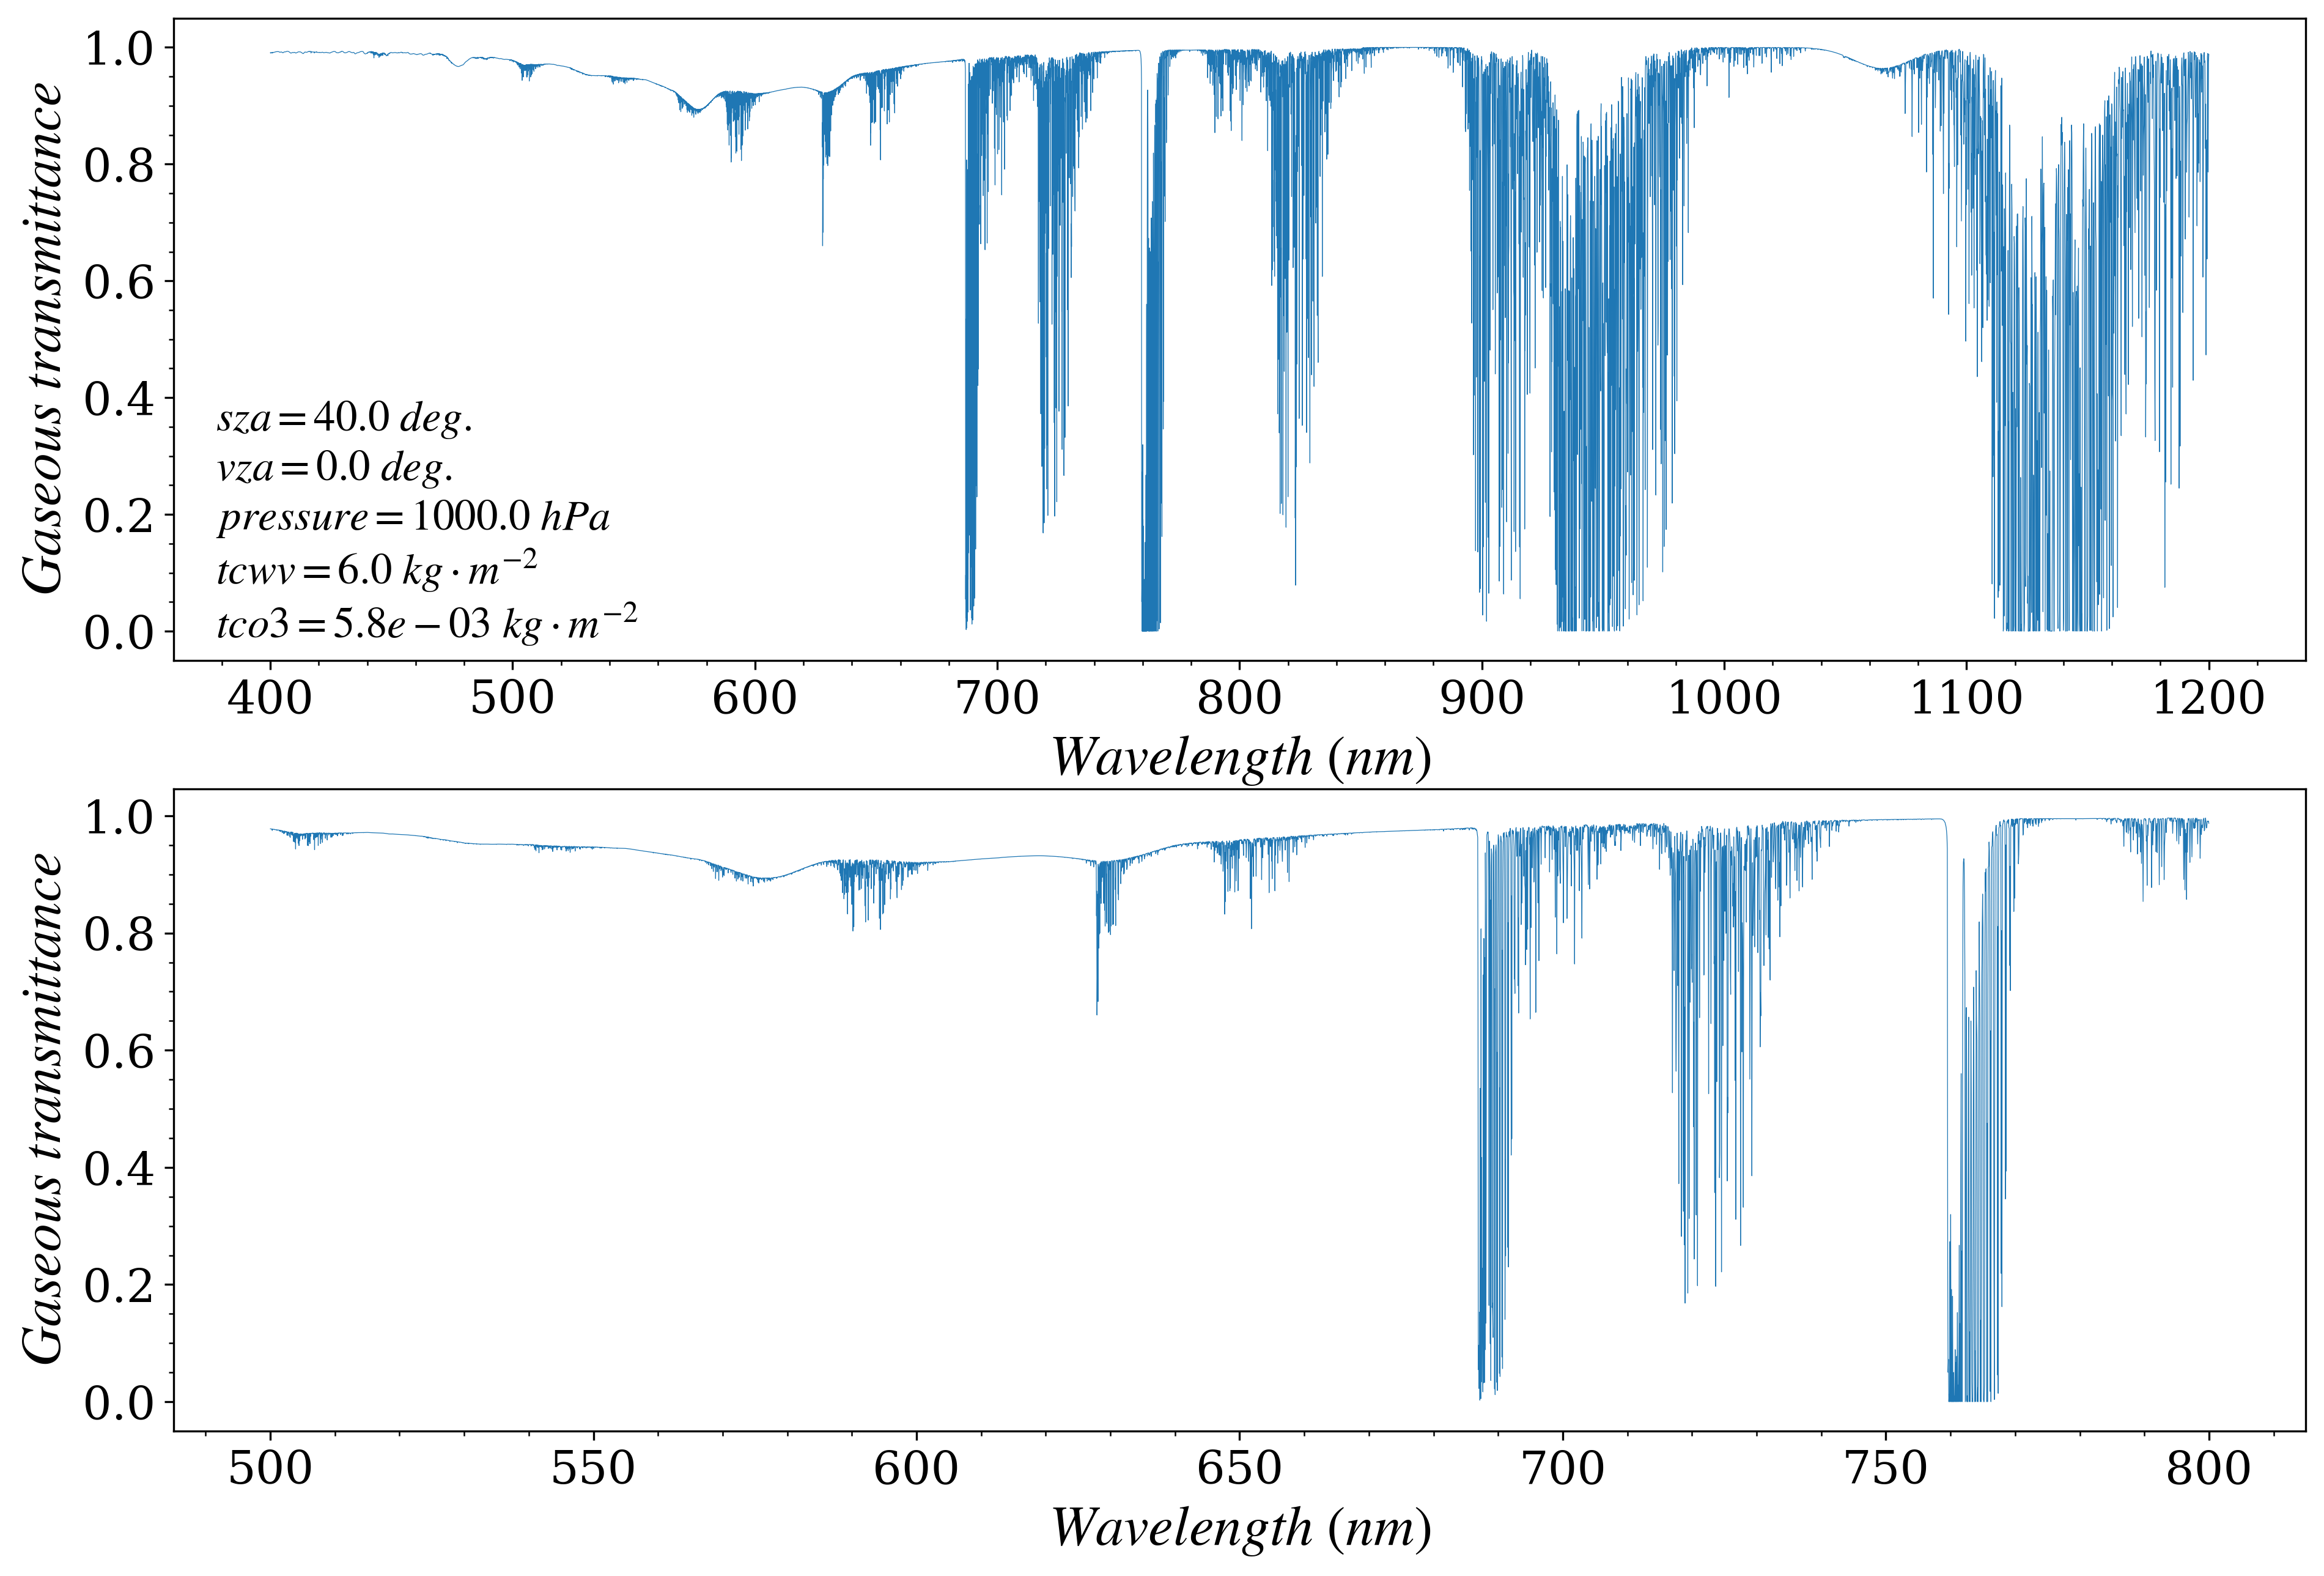
\includegraphics[width=0.8\linewidth]{abs_transmittance_hyperspectral.png}
    \caption{Example of the hyperspectral transmittance computed from L2A Sentinel-3 atmospheric products, see values in top panel.}
    \label{fig:computed_trans}
\end{figure}

\subsubsection{Line-by-line absorption of O$_2$}\label{sec:o2_lbl}
The REPTRAN parameterization of the gaseous absorption (fine table of about 0.06 nm) is made for spectral bands of a few
nanometres. At the sub-nanometre resolution of FLEX, the absorption of O$_2$ in the O$_2$-B (683--702 nm) and O$_2$-A
(755--775 nm) bands is computed line by line from the HITRAN line parameters, averaged in the cells of the gaseous table.
Compared with the line-by-line computation, REPTRAN overestimates the absorption at 0.3 nm resolution: the transmittance
of the O$_2$-B band head is about halved and the lines of the P branch of the O$_2$-A band are deeper
(Figure \ref{fig:o2_lbl}).

\begin{figure}[H]
    \centering
    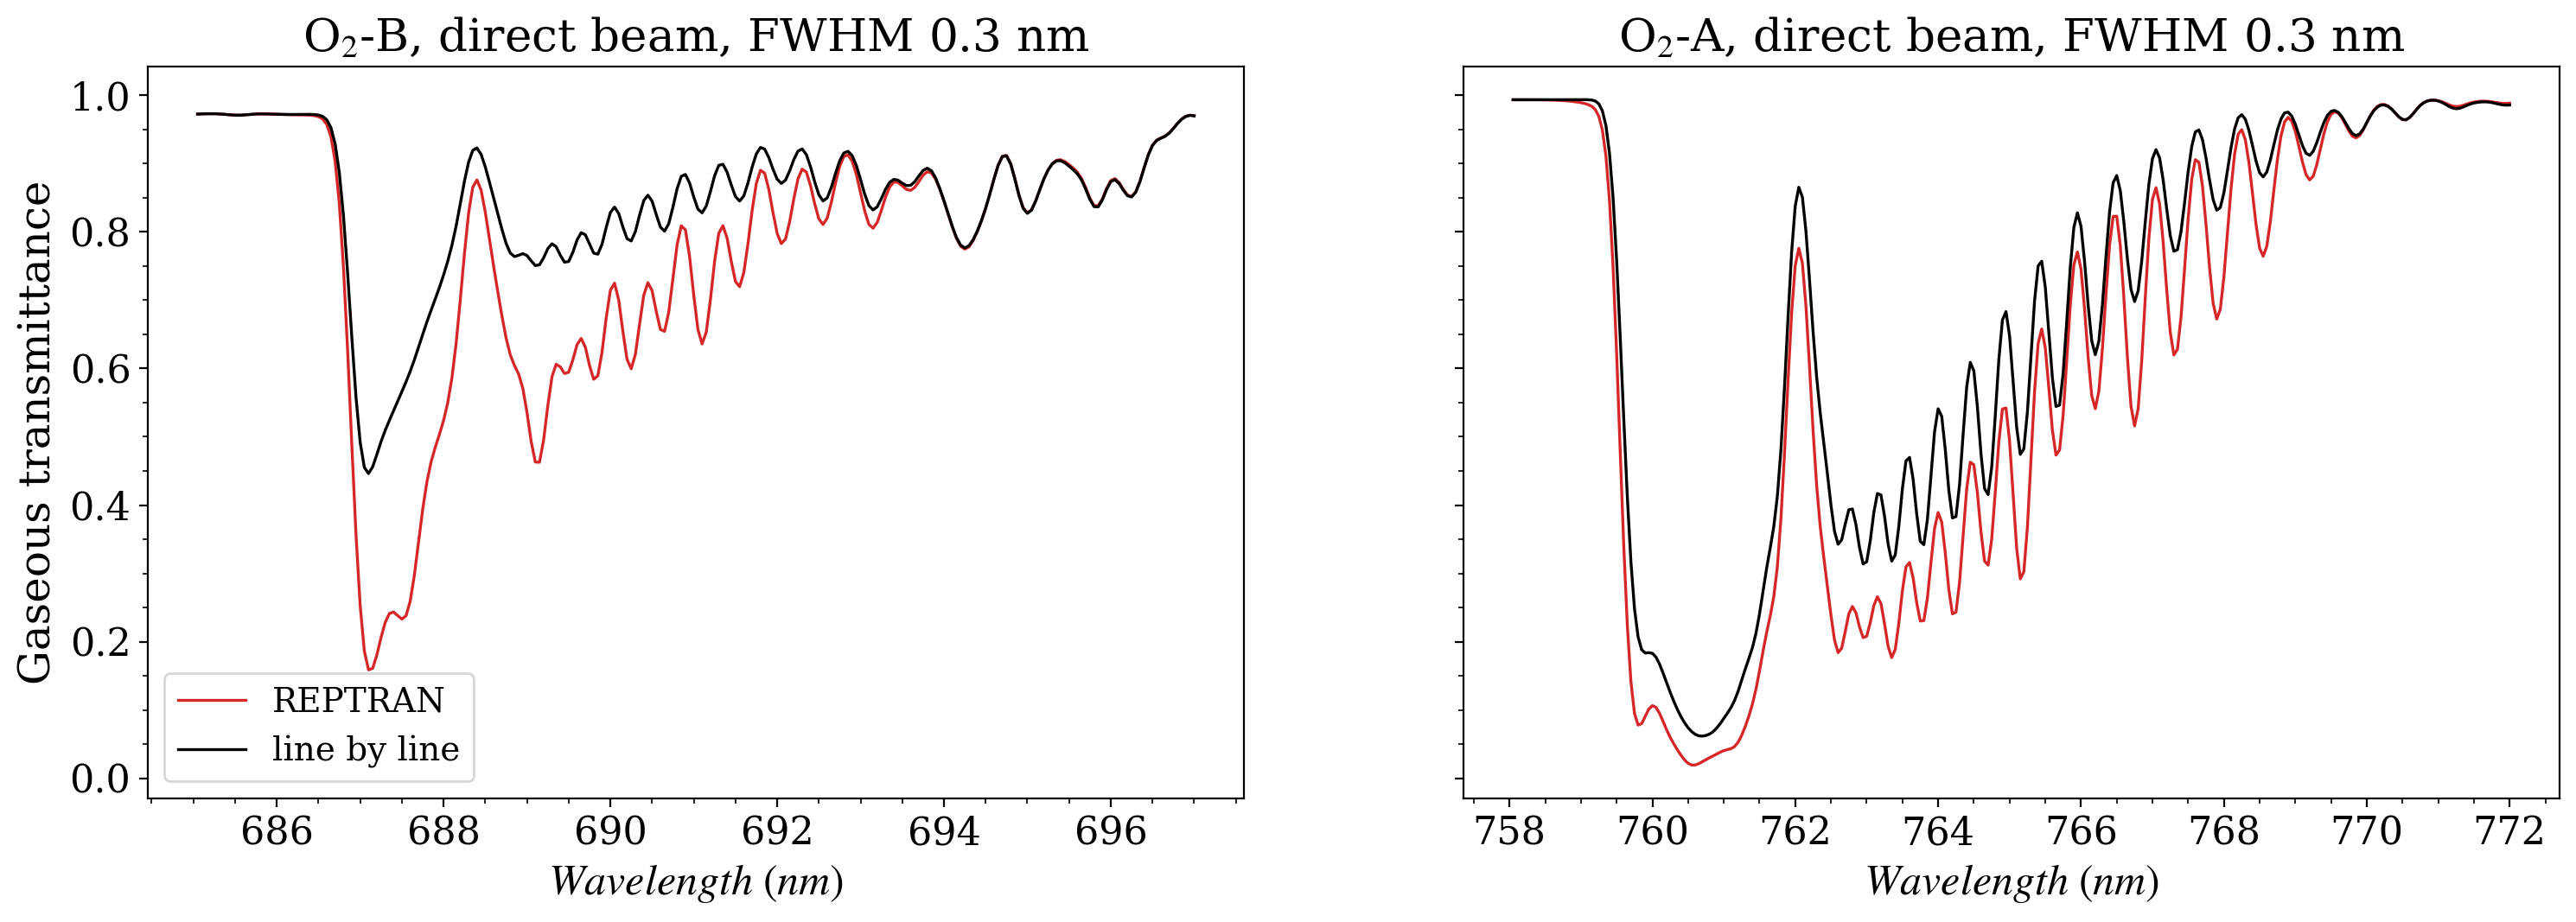
\includegraphics[width=0.95\linewidth]{o2_lbl_reptran_flex.png}
    \caption{Transmittance of the direct beam (Sun-surface-sensor path) in the O$_2$-B and O$_2$-A bands at 0.3 nm resolution
    (Gaussian responses): line-by-line O$_2$ (black) and REPTRAN (red), atmosphere of the bloom pixel of Section \ref{sec:performance}.}
    \label{fig:o2_lbl}
\end{figure}

\subsubsection{Coupling of the gaseous absorption with the scattering}\label{sec:coupling}
The transmittance $T_g(\lambda, m)$ of the direct beam, for the geometric air mass $m$, is exact for the direct light only.
The photons scattered by the molecules and aerosols do not cross the same amount of absorbers: the photons scattered above
the absorbers shortcut part of the path, which reduces the absorption of the path reflectance, especially for the water
vapour concentrated in the lowest kilometres, while the skylight reaching the surface travels longer paths, which slightly
increases the absorption of the water-leaving term and of the downwelling irradiance. This coupling was quantified with the
SOS-ABS radiative transfer code (Successive Orders of Scattering coupled with the gaseous absorptions,
\url{https://github.com/CNES/RadiativeTransferCode-SOS}, correlated-$k$ distributions) and is parameterized, for each term
$X \in \{atm, w, E_d\}$, by a photon path-length model (Gamma distribution of the absorber paths, equivalence theorem):
\begin{equation}
T_g^{X}(\lambda) = \left(1 + s_X^2\, \eta_X\, \tau_g(\lambda, m_X)\right)^{-1/s_X^2},
\qquad \tau_g(\lambda, m) = -\ln T_g(\lambda, m),
\label{eq:ppld}
\end{equation}
with $m_{atm} = m_w = 1/\mu_0 + 1/\mu_v$ and $m_{E_d} = 1/\mu_0$. The mean absorber path relative to the geometric one,
$\eta_X$, and its relative variance, $s_X^2$, are fitted per absorption window and term on the SOS-ABS simulations, as
functions of the air mass, the aerosol optical thickness and the water vapour column. The model is applied channel by
channel (line by line in the O$_2$ bands) to the water vapour and the background gases in the O$_2$ and H$_2$O bands of
684--990 nm; elsewhere $T_g^X = T_g(\lambda, m_X)$. The path reflectance sees only a fraction of the geometric path
($\eta_{atm} \approx 0.45$--$0.65$), the water-leaving term and the irradiance slightly more ($\eta \approx 1.02$--$1.05$).
For $\eta_X = 1$ and $s_X^2 \to 0$ (decoupled model), the band-averaged TOA reflectance is underestimated by about 4\,\% in
the O$_2$-B band, 10--15\,\% at 720, 820 and 900 nm, 30\,\% in the O$_2$-A head and 50--60\,\% in the 940 nm band
(RadCalNet-OC 1.1, \url{https://radcalnet-oc.readthedocs.io}).

At the resolution of FLEX, the coupling mainly concerns the path reflectance: for the atmosphere of the bloom pixel of
Section \ref{sec:performance}, $T_g^{atm}$ is on average 6\,\%, 13\,\% and 36\,\% larger than the transmittance of the
direct beam in the O$_2$-B, H$_2$O (720 nm) and O$_2$-A windows, and up to 4.4 times larger in the core of the O$_2$-A band,
while $T_g^{w}$ differs from it by less than 2.5\,\% (Figure \ref{fig:gas_coupling}). The atmospheric reflectance to be
removed is changed by up to 31\,\%, 58\,\% and 340\,\% in these windows (Figure \ref{fig:ratm_coupling}).

\begin{figure}[H]
    \centering
    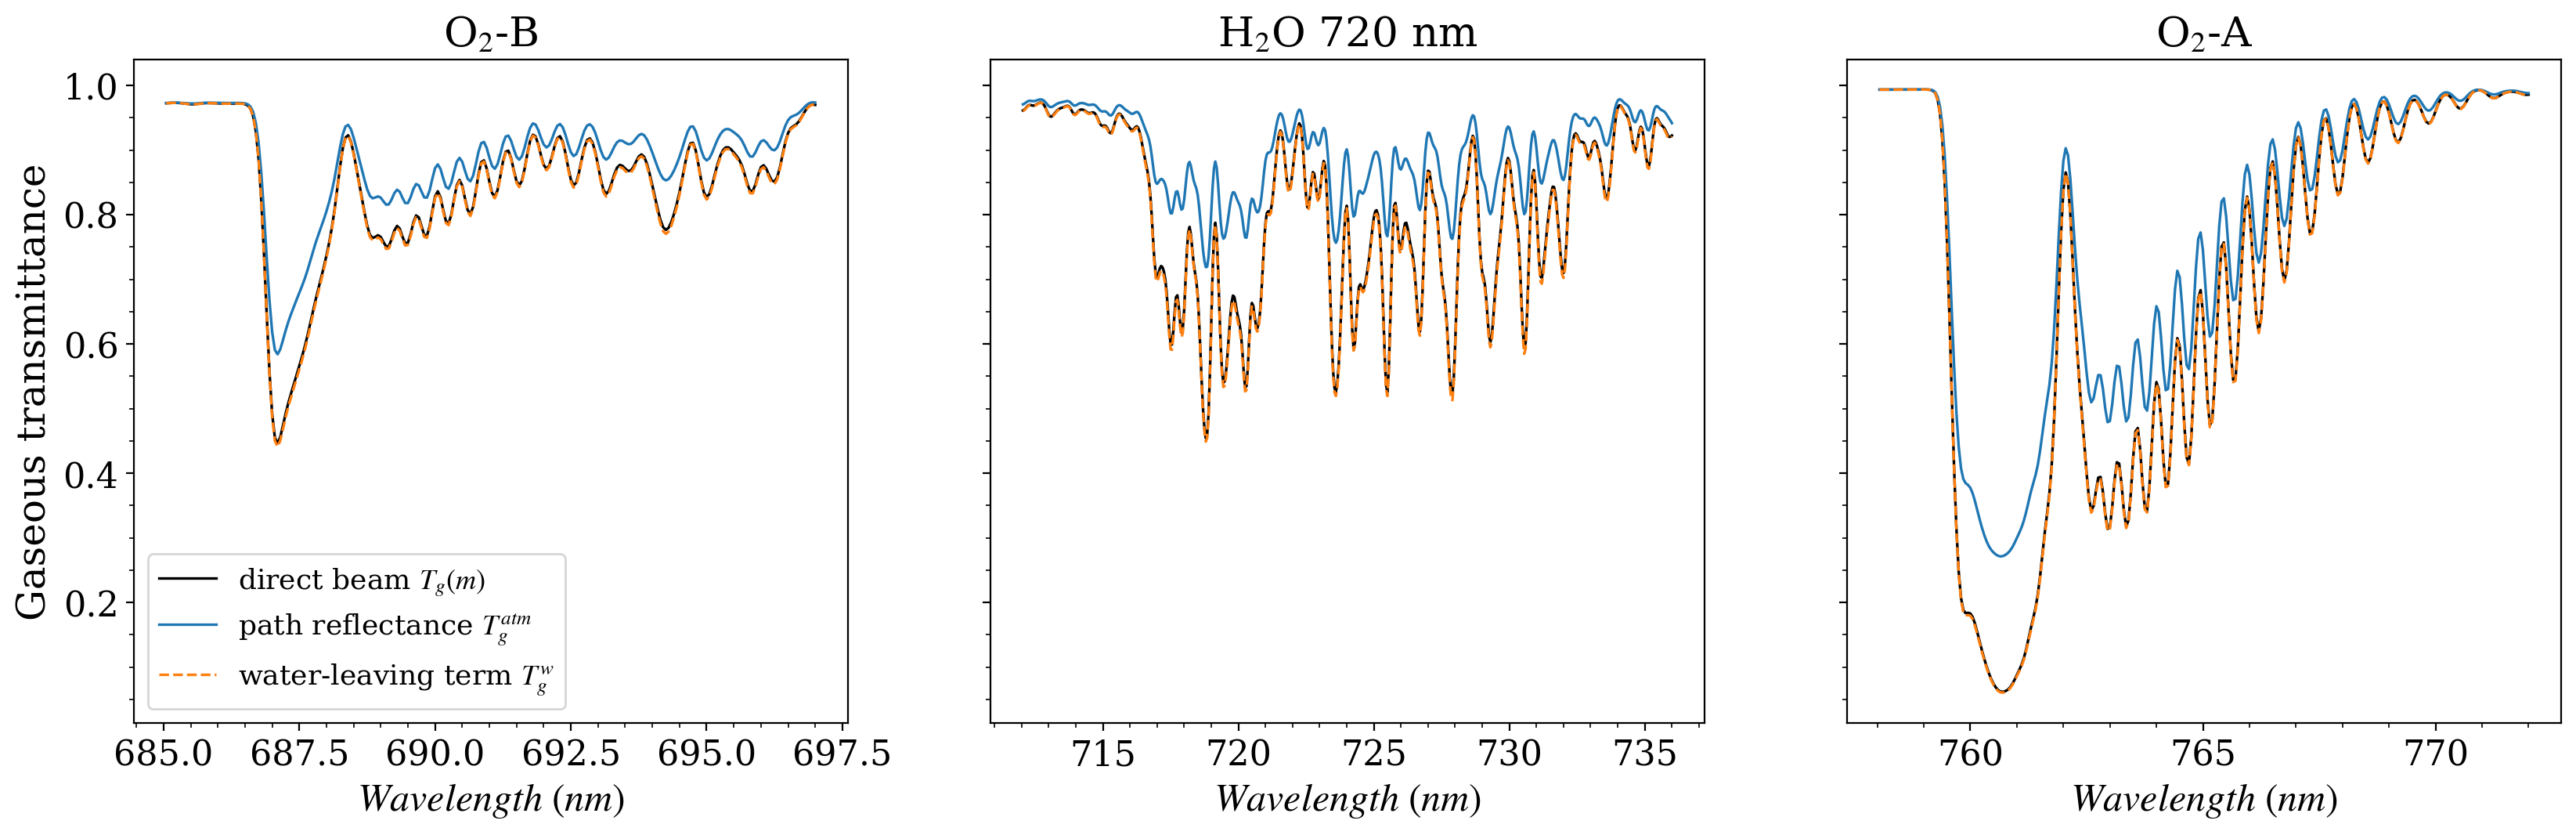
\includegraphics[width=1\linewidth]{gas_coupling_flex.png}
    \caption{Gaseous transmittances at 0.3 nm resolution in the O$_2$-B, H$_2$O (720 nm) and O$_2$-A windows: direct beam of the
    Sun-surface-sensor path $T_g(m)$ (decoupled model) and transmittances coupled with the scattering of the path reflectance
    $T_g^{atm}$ and of the water-leaving term $T_g^{w}$ (photon path-length model), atmosphere and geometry of the bloom pixel.}
    \label{fig:gas_coupling}
\end{figure}

\begin{figure}[H]
    \centering
    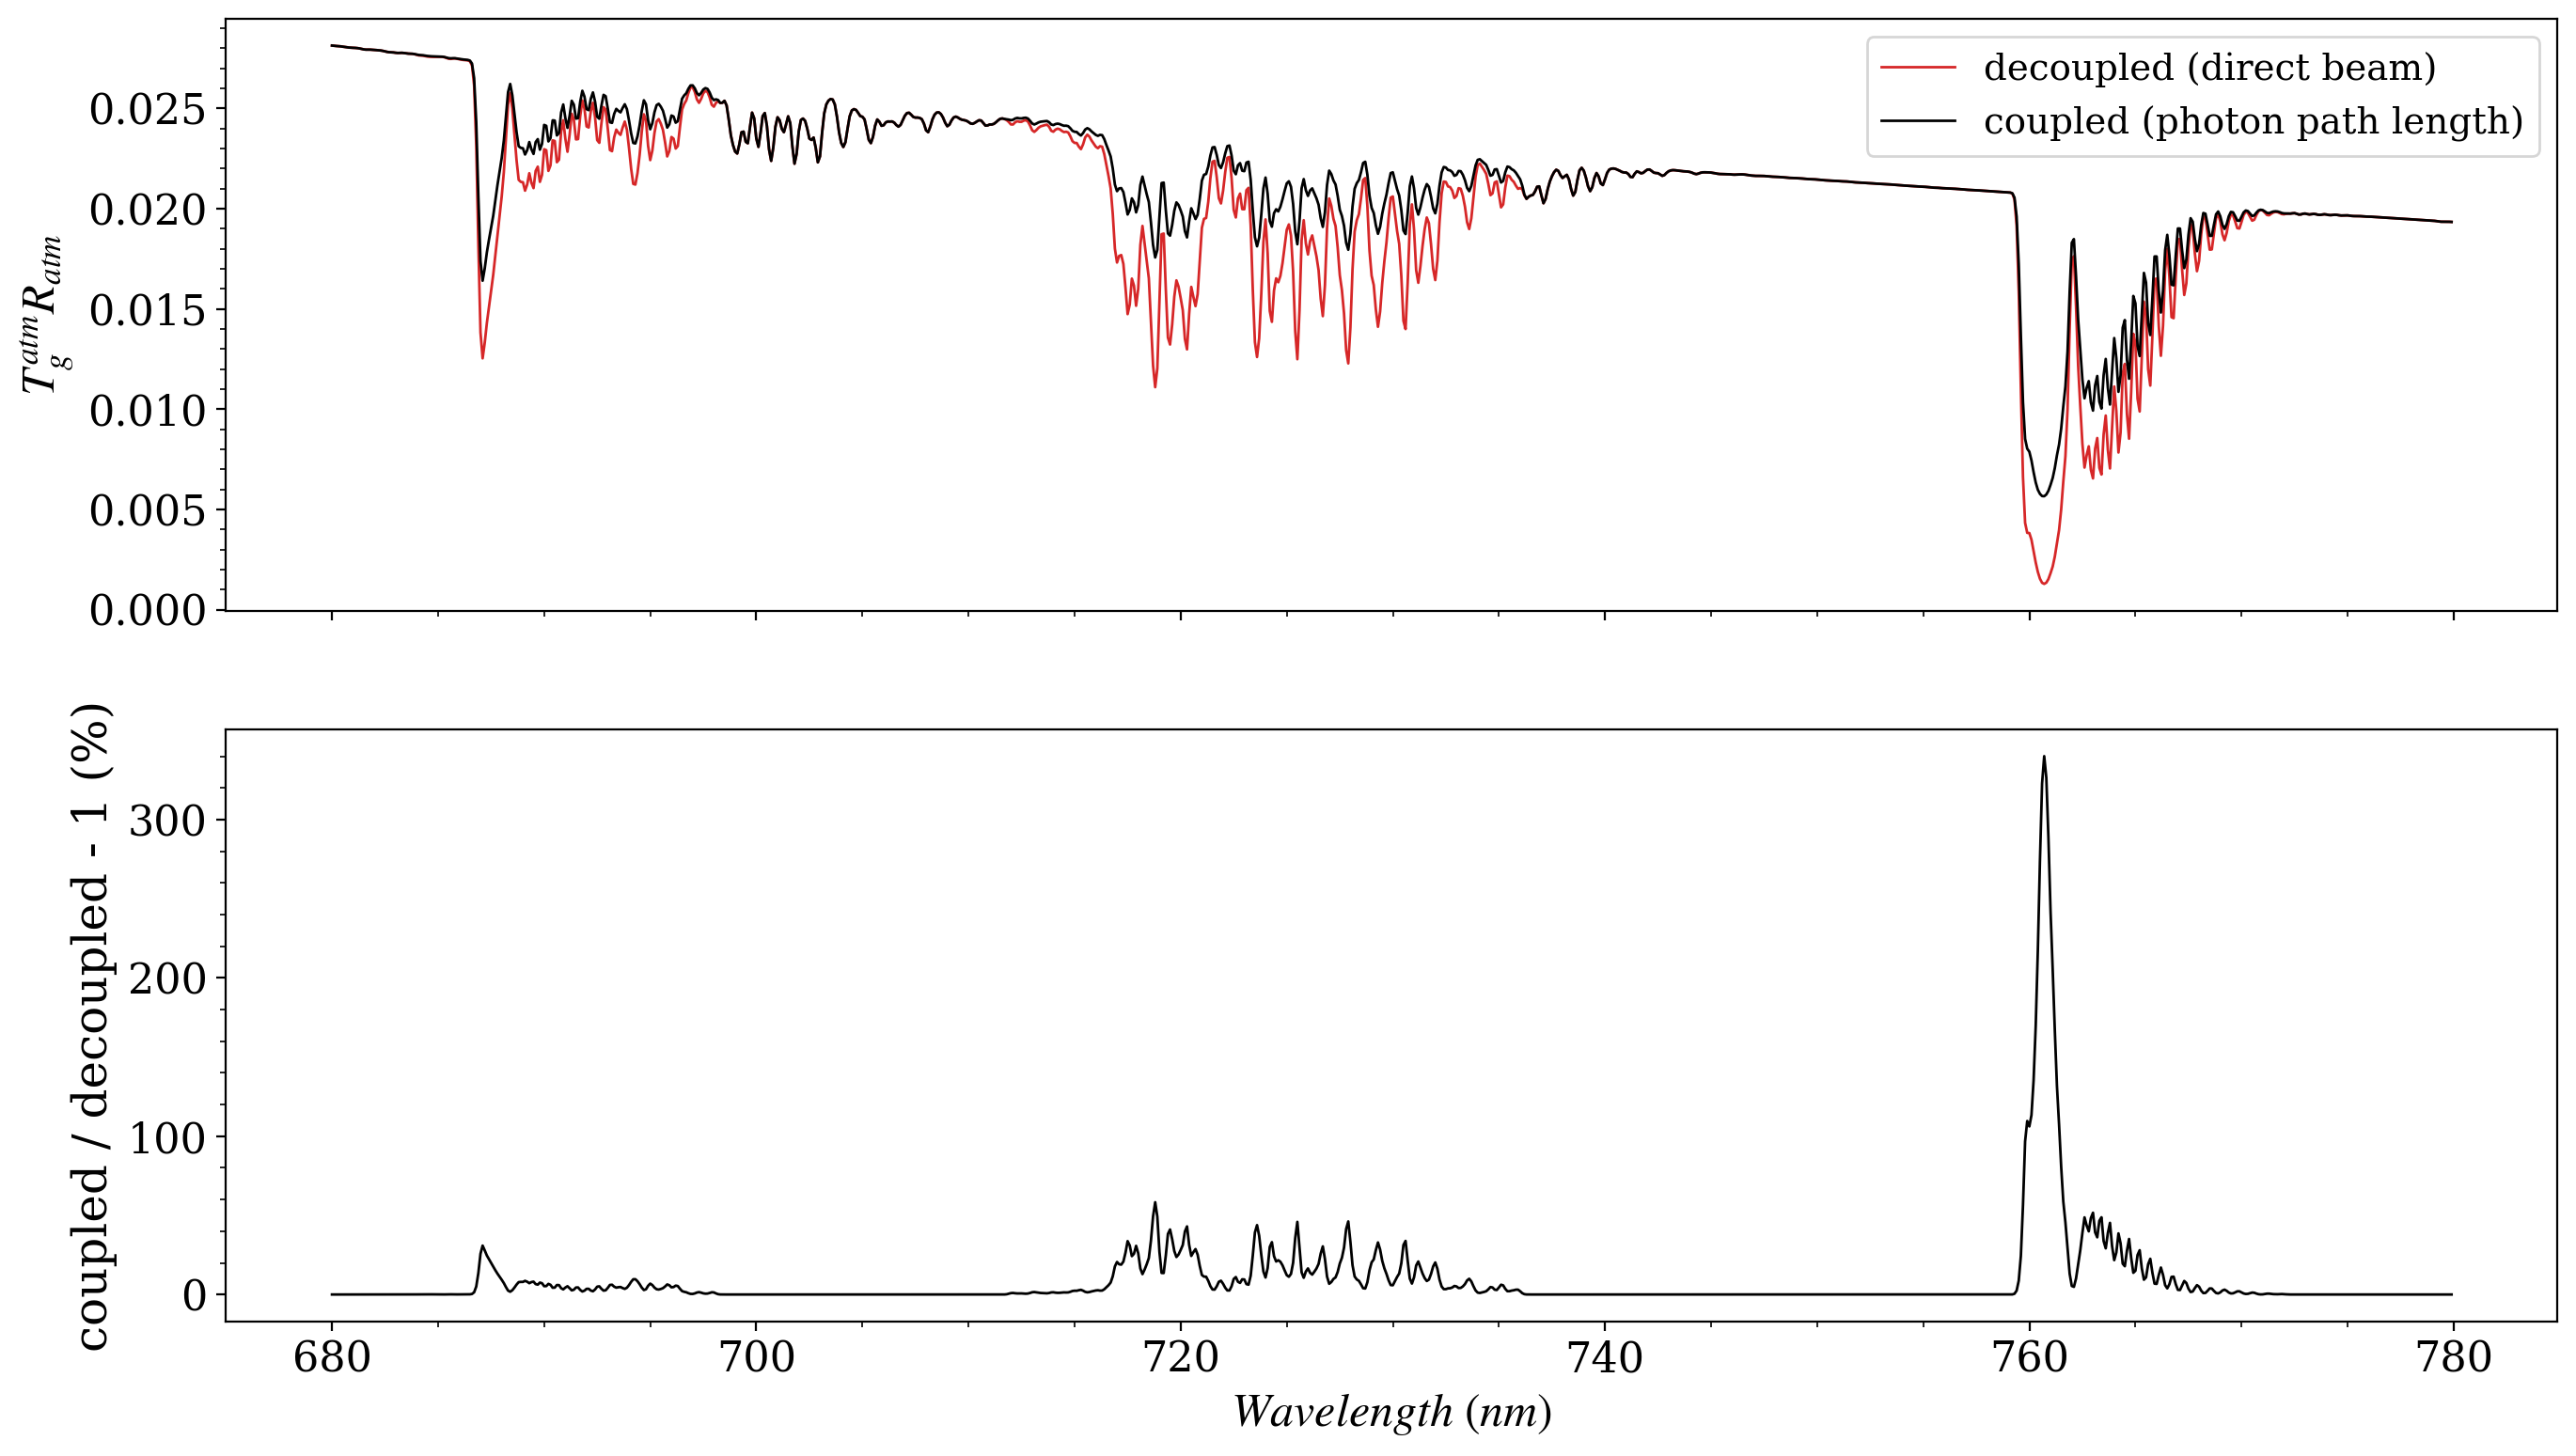
\includegraphics[width=0.9\linewidth]{ratm_gas_coupling_flex.png}
    \caption{Atmospheric reflectance at the TOA, $T_g^{atm} R_{atm}$, of the bloom pixel at 0.3 nm resolution, with the coupled
    (black) and decoupled (red) gaseous transmittances (top), and relative difference (bottom).}
    \label{fig:ratm_coupling}
\end{figure}

\subsection{Sunglint model}

The sunglint component of the measured radiance, $L_{g}^{TOA}$, can be straightforwardly formulated as follows:
   \begin{equation}                                                                             	
L_{g}^{TOA}\left( {{\theta }_{s}},{{\theta }_{v}},\Delta \varphi  \right)={{T}_{u}}\left( {{\theta }_{v}} \right)BRD{{F}_{g}}\left( {{\theta }_{s}},{{\theta }_{v}},\Delta \varphi  \right){{T}_{d}}\left( {{\theta }_{s}} \right)L_{sun}^{\downarrow }\left( {{\theta }_{s}} \right)
,                                           
\label{eq:placeholder}
\end{equation}
where $L_{sun}^{\downarrow }$ is the extraterrestrial sun radiance reaching the atmosphere, $T_d$ and $T_u$ are the downward and upward direct transmittance, respectively, and $BRDF_{g}$ is the bidirectional reflectance distribution function of the rough water surface.

If the ocean surface is roughened by the wind, a myriad of reflected images of the sun will reach the satellite sensor due to specular reflection from various waves and wavelets of the sea surface. Following Cox and Munk \cite{Cox1954a,Cox1956}, the ocean surface can be modeled based on a distribution of small facets. The orientation of the facets can be fully described by their slopes $\zeta_x$ and $\zeta_y$ along the $x$ and $y$ axis of Figure \ref{fig:geometry}. The slopes $\zeta_x$ and $\zeta_y$  of facets contributing to sun light reflection toward the satellite sensor (sunglint signal) can be expressed based on the viewing configuration as follows:

\begin{equation}
\begin{cases}
  & {{\zeta }_{x}}=\frac{\partial z}{\partial x}={-\left( \sin {{\theta }_{s}}+\sin {{\theta }_{v}}\cos \Delta \varphi  \right)}/{\left( \cos {{\theta }_{s}}+\cos {{\theta }_{v}} \right)}\;, \\
 & {{\zeta }_{y}}=\frac{\partial z}{\partial y}={-\left( \sin {{\theta }_{v}}\cos \Delta \varphi  \right)}/{\left( \cos {{\theta }_{s}}+\cos {{\theta }_{v}} \right).}\; \\

\end{cases}
\label{eq:placeholder}
\end{equation}

The proportion of such facets can be related to the wave slopes distribution. In addition, an accurate parameterization of the sunglint requires the consideration of the multiple reflections on the wave facets \cite{Ottaviani2008a, Li2013a} and of wave shadowing effects \cite{Ross2005}, which depend on the wave height $h$. Several studies introduced different formulations of a function $q$ which merges the wave slope distribution with observable effects of multiple reflections and shadowing \cite{Plass1975,Ross2005}. Whatever the parameterization of $q$, the BRDF of the air/water interface can be formulated as follows:
\begin{equation}
BRDF_{g}=\frac{\pi {{R}_{f}}\left( \omega  \right)}{4\cos {{\theta }_{v}}\cos ^{4}{{\theta }_{N}}}q\left( {{\zeta }_{x}},{{\zeta }_{y}},h \right)
\label{eq:placeholder}
\end{equation}       	                    	
where $R_f$ is the Fresnel reflection coefficient and $\omega$ the angle of incidence of the sun ray on any wave facet continuing to the sunglint along the viewing direction. Note this equation is applicable to a point source, it has been shown that the use of the Sun’s irradiance produces an error smaller than 1 \% on the resulting observed reflected radiance for any slope variance as long as the Sun is more than $10^\circ$ above the horizon \cite{Ross2005}.  The angle of incidence is defined as follows:
\begin{equation}
  \cos{2\omega}=\cos{\theta_s}\cos{\theta_v}+\sin{\theta_s}\sin{\theta_v}\cos{\Delta\varphi} 
 \label{eq:placeholder}
\end{equation}
To be complete, the model takes into account the wind direction impact on the sunglint reflectance. Let us introduce the upwind (\textit{up}) and crosswind (\textit{cr}) components of the sea surface slope:
\begin{equation}
\begin{cases}
 \zeta_{up}=\zeta _{x} \cos\phi_{wind}+\zeta _{y} \sin\phi_{wind}\\
 \zeta_{cr}=\zeta _{y} \cos\phi_{wind}- \zeta _{x} \sin\phi_{wind}

\end{cases}
\label{eq:placeholder}
\end{equation}
where $\phi_{wind}$ is the azimuth of the upwind direction with respect to the Sun direction. Finally, the wave slope distribution might be expressed based on a \textit{Gram-Charlier} decomposition, as follows:
\begin{equation}
q(\zeta_{up}, \zeta_{cr}) = \frac{1}{2\pi\sigma_{up}\sigma_{cr}} \exp\left(-\frac{\xi^2 + \eta^2}{2}\right)\\
\left[\begin{array}{l}\,1 - \frac{1}{2} c_{21}(\xi^2 - 1)\eta \\\,- \frac{1}{6} c_{03}(\eta^3 - 3\eta) \\\,+ \frac{1}{24} c_{40}(\xi^4 - 6\xi^2 + 3) \\\,+ \frac{1}{24} c_{04}(\eta^4 - 6\eta^2 + 3) \\\,+ \frac{1}{4} c_{22}(\xi^2 - 1)(\eta^2 - 1)\\\end{array}\right]
\label{eq:placeholder}
\end{equation}
where $\sigma_{up}$ and  $\sigma_{cr}$ are the upwind and crosswind root mean square slopes, $\eta=\zeta_{up}/\sigma_{up}$ and $\xi=\zeta_{cr}/\sigma_{cr}$. The $c_{ij}$ are the coefficients quantifying the non-Gaussian nature of the distribution, the specific values used can be found in the \textit{coxmunk} python package here \url{https://github.com/Tristanovsk/coxmunk}. Figure \ref{fig:sunglint} shows the computed sunglint reflectance for a sun zenith angle of 35° and a wind azimuth $\phi_{wind}$ of 0° for several wind speeds to illustrate the typical directional signature of the sunglint component of the signal.
\begin{figure}
    \centering
    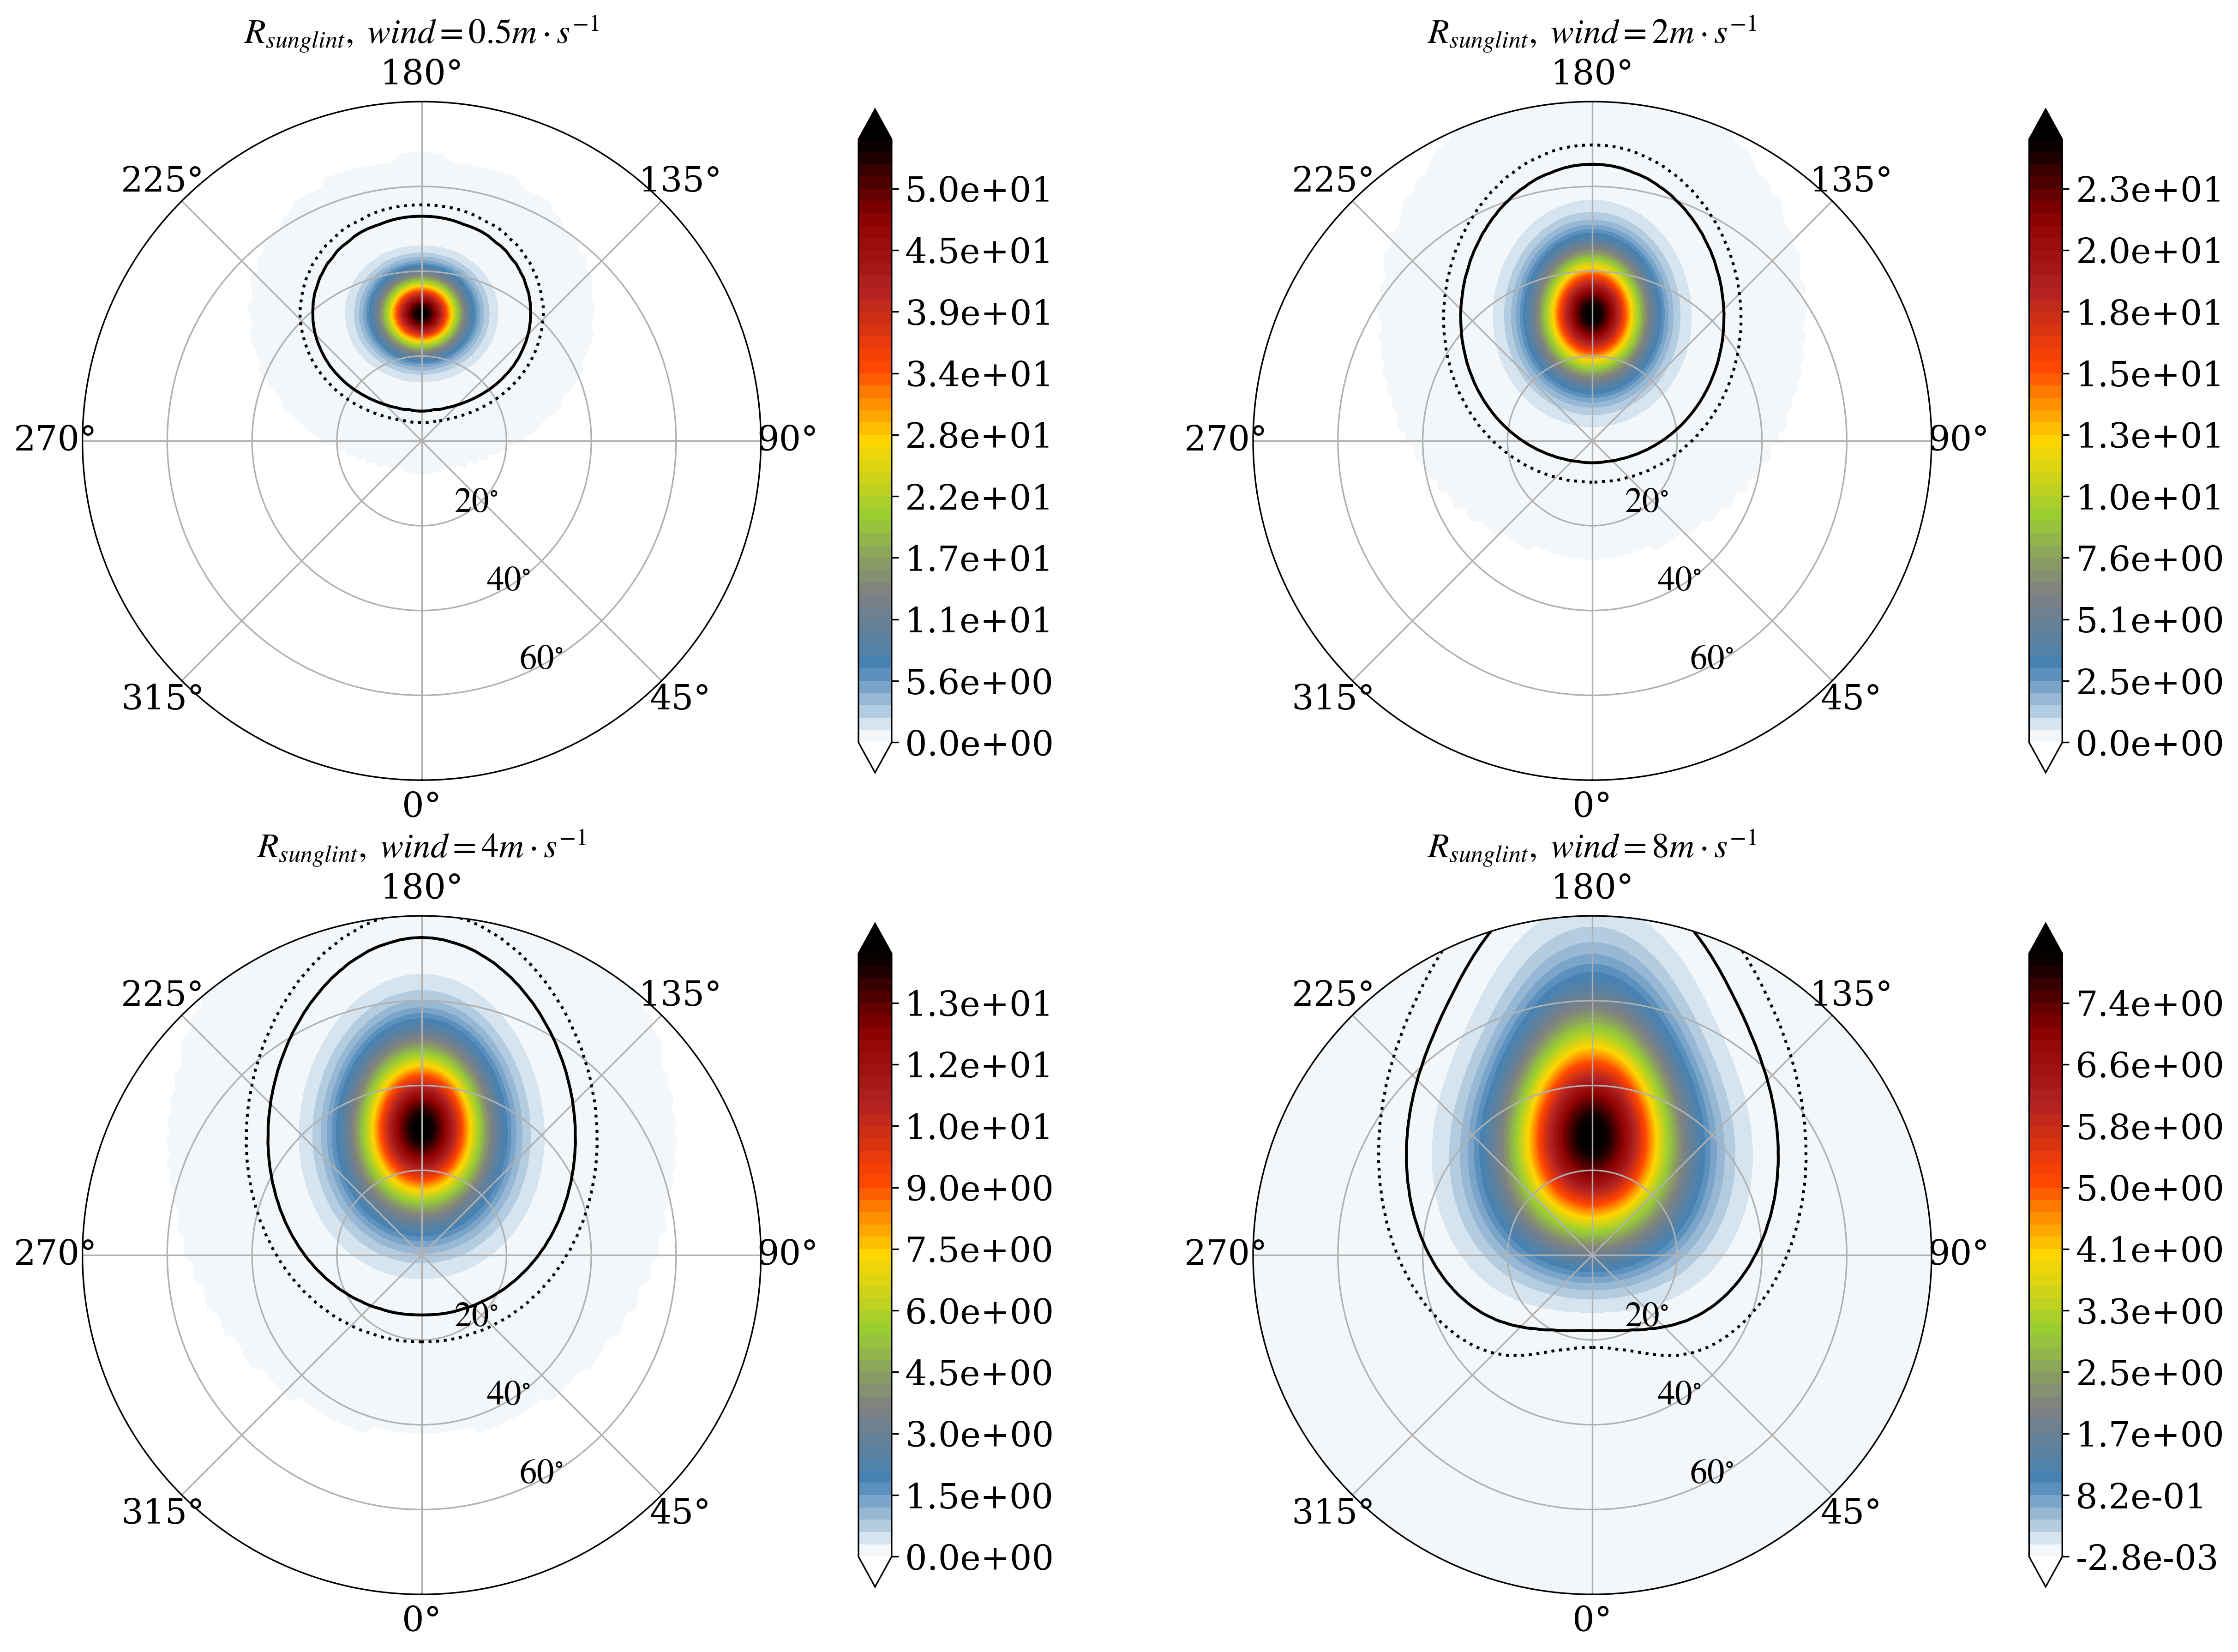
\includegraphics[width=0.85\linewidth]{Rsunglint_bh2006_wazi0.png}
    \caption{Directional values of the $BRDF_{g}$ for several wind speeds (from 0.5 to 8 $m\cdot s^{-1}$) computed from Breon and Henriot \cite{Breon2006} statistics. The continuous end dotted black lines represent the isolines of 5\% and 1\%, respectively.}
\label{fig:sunglint}
\end{figure}

Now, including the impact of direct transmission within the atmosphere, the figure \ref{fig:Rtoa_sunglint} shows the sunglint spectral reflectance at the top-of-atmosphere level for different aerosol loads and types. It is readily observed that not only the aerosol load but also the types of aerosols significantly impact the sunglint signature. This demonstrates the need for accurate aerosol retrieval in parallel of the sunglint correction within the atmospheric correction algorithm, see section \ref{sec:sunglint_pixel}.  The figure \ref{fig:Rtoa_diff_sunglint} shows the proportion of diffuse light and sunglint in the satellite signal.
\begin{figure}[H]
    \centering
    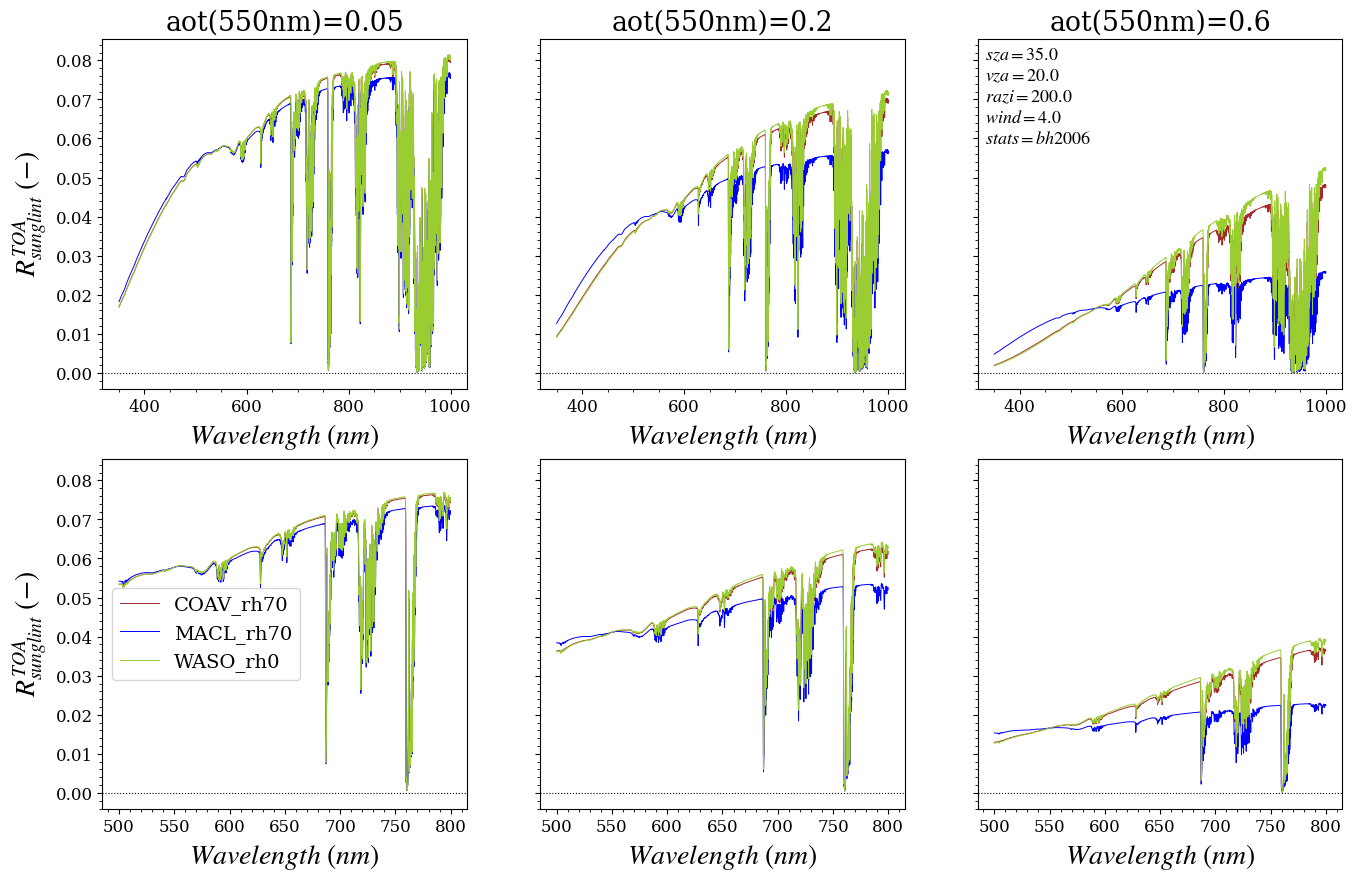
\includegraphics[width=0.95\linewidth]{sunglint_aerosol_model.png}
    \caption{Simulation of the sunglint reflectance at the top of the atmosphere for various aerosol loads and types: (top row) for the spectral range of Sentinel-3 OLCI, (bottom row) for spectral range of FLEX}
    \label{fig:Rtoa_sunglint}
\end{figure}


\begin{figure}[htb]
    \centering
    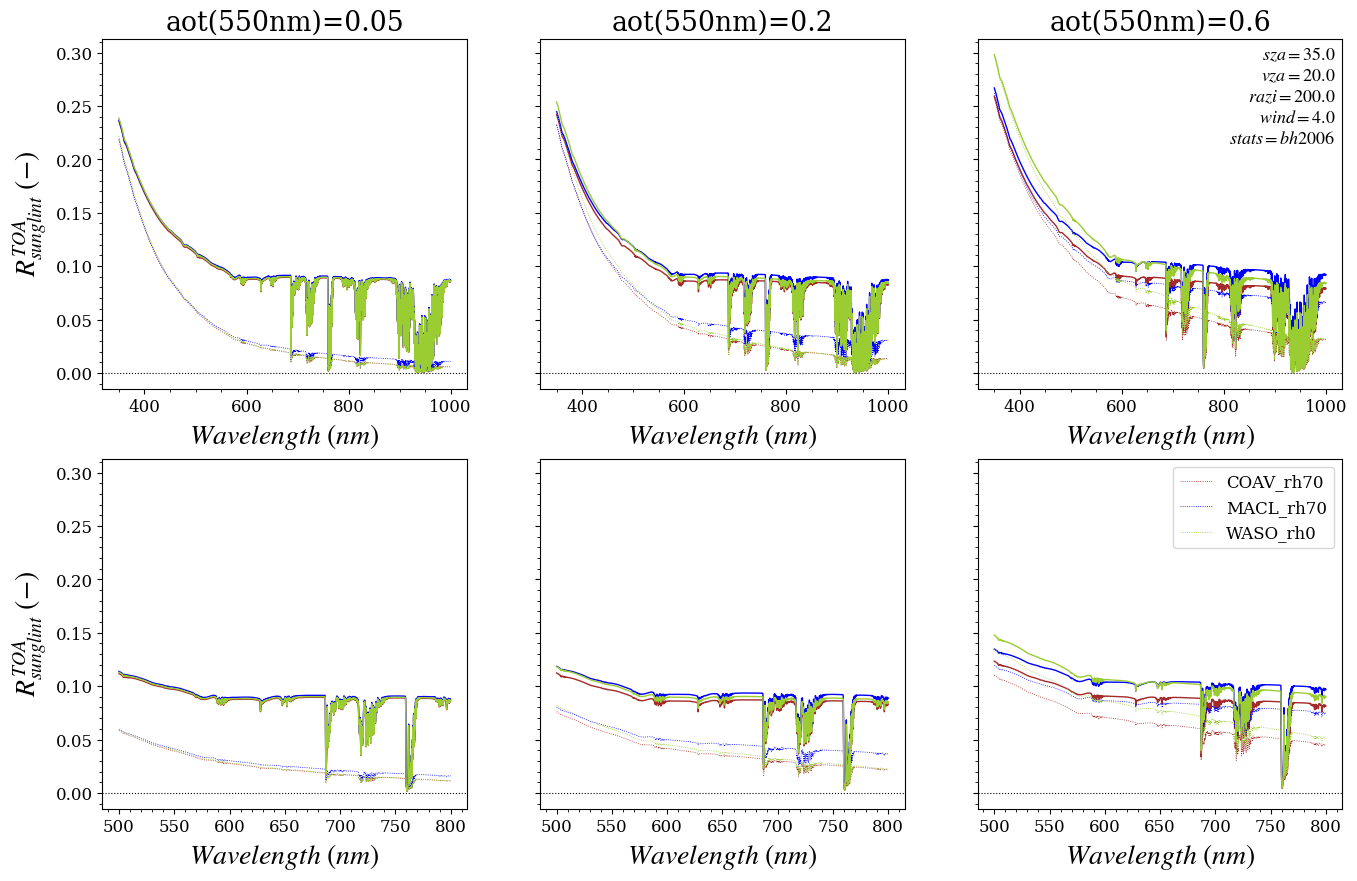
\includegraphics[width=0.95\linewidth]{Rsunglint_Rtoa.png}
    \caption{Similar to Fig. \ref{fig:Rtoa_sunglint} displaying the diffuse reflectance (dotted lines) and the total reflectance (diffuse + sunglint, continuous lines)}
    \label{fig:Rtoa_diff_sunglint}
\end{figure}
\section{Generation of look-up tables}
\subsection{Solar irradiance}
As already mentioned, the solar irradiance reference is taken from TSIS \cite{Coddington2023}, see Figure \ref{fig:solar_ref}. Nevertheless, the extraterrestrial solar irradiance needs to be corrected for the ellipticity of the Earth orbit. Here, we use the Earth-Sun distance correction factor, the ratio squared ratio of mean radius $R_0$ over actual radius $R_t$,  for adjustment of mean solar irradiance $\overline{E_0}$, as follows:
\begin{equation}
   E_0=\overline{E_0} \left(\frac{R_0}{R_t}\right)^2 
\label{eq:earth_sun}
\end{equation}
with
\begin{equation}
\left(\frac{R_0}{R_t}\right)^2 = 1.00011 + 0.034221\cos\theta + 0.00128 \sin\theta + 
             0.000719 \cos2 \theta + 0.000077 \sin2\theta
\label{eq:earth_sun_radius}
\end{equation}
and
\begin{equation}
\theta = 2\pi \frac{DOY}{365}
 \label{eq:day_earth_sun}
\end{equation}
with $DOY$ the day of year number.       

\subsection{LUT files and format}\label{sec:lut}
The code OSOAA \cite{Chami2015} was used to generate the diffuse reflectances and transmittances of the atmosphere-surface system based on the aerosol models previously described, aerosol optical thicknesses ranging from 0 to 0.8 at 550 nm, and a comprehensive set of viewing geometries ($\theta_s, \theta_v, \Delta\varphi$) .  All the output parameters of interest have been stored in look-up tables (LUT) as a \textit{netcdf} file as illustrated in Figure \ref{fig:lut_aero}. Within the algorithm, the LUT values are interpolated at the spectral resolution of FLEX for the specific viewing geometry of the pixels, and linearly between the wind speeds of the LUT (0.5 to 16 $m\cdot s^{-1}$) at the wind speed of the L2A product. Regarding the absorption properties of atmospheric gases the optical thicknesses of the different molecules of interest are store in a netcdf file with \~0.2 nm spectral resolution, see Figure \ref{fig:lut_gas}.

\begin{figure}[H]
    \centering
    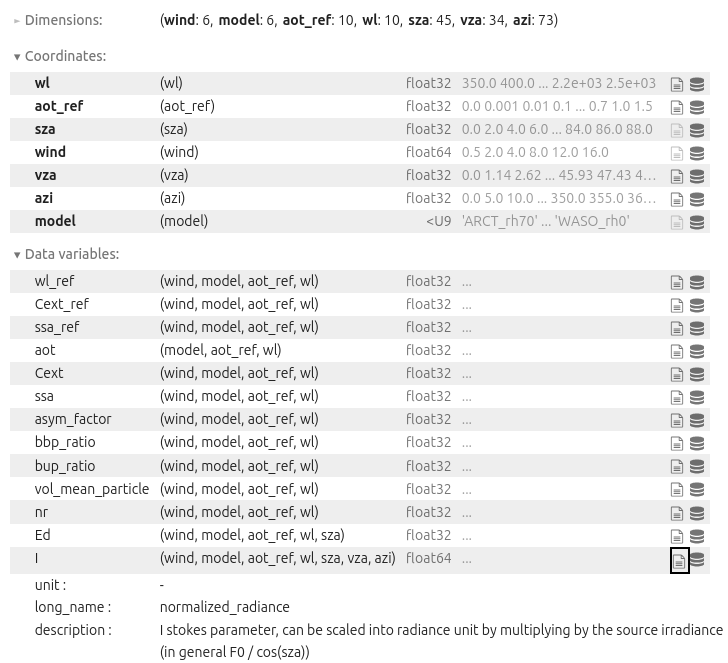
\includegraphics[width=0.75\linewidth]{lut_aero.png}
    \caption{Look-up table generated using OSOAA radiative transfer code for several aerosol loads and types.}
    \label{fig:lut_aero}
\end{figure}

\begin{figure}[h]
    \centering
    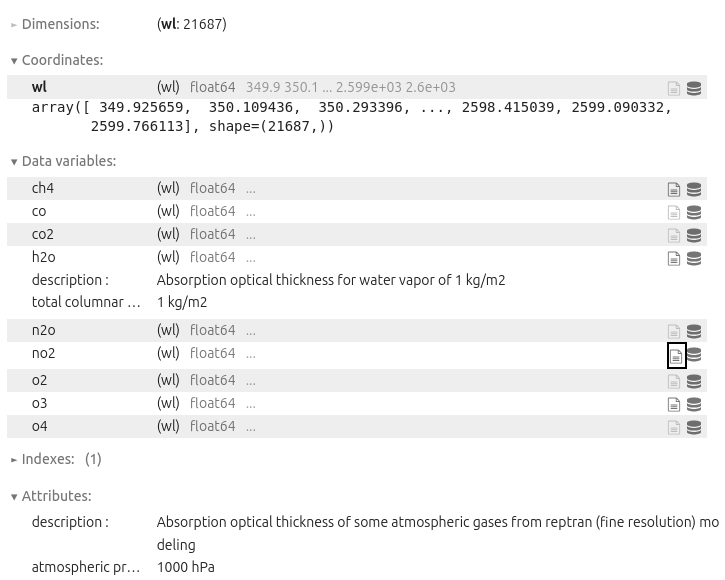
\includegraphics[width=0.75\linewidth]{lut_gas.png}
    \caption{Look-up table of the absorbing gases absorption optical thickness.}
    \label{fig:lut_gas}
\end{figure}

\subsection{Downwelling irradiance and photosynthetically available radiation}
Thanks to the RadCalNet-OC package (\url{https://radcalnet-oc.readthedocs.io}) based on the previously described equations, the downwelling irradiance can be computed from the input parameters from L2A Sentinel-3 product (or directly estimated through non-linear optimization, in the future). In the following figure, the top-of-atmosphere and bottom-of-atmosphere downwelling irradiance are shown for various spectral resolution based on convolution with the instrumental spectral responses through FWHM (i.e., full width at half maximum of Gaussian-like distribution). In the implemented algorithm, the resolution at 1-nm is provided as output product after atmospheric correction.
    \begin{figure}[H]
    \centering
    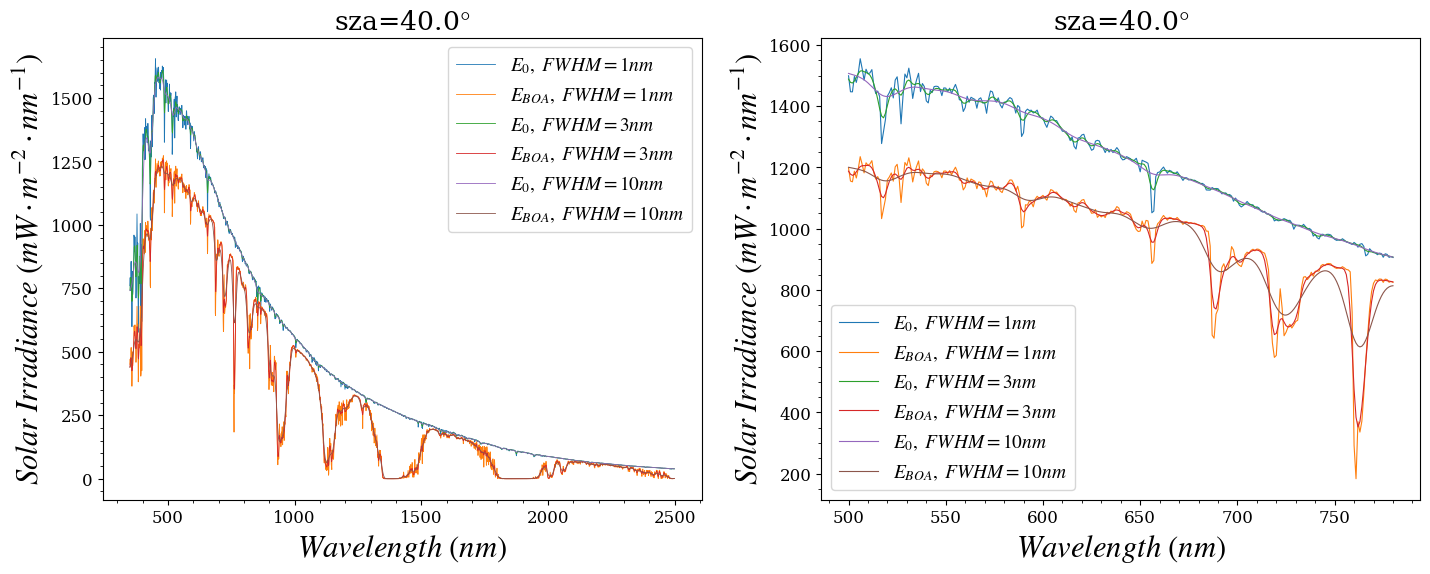
\includegraphics[width=0.85\linewidth]{solar_irr_fwhm_sza40.png}
    \caption{Solar irradiance}
    \label{fig:toa_boa_ed}
\end{figure}
Besides spectrally resolved downwelling irradiance, it is also of interest to provide estimates of PAR (Photosynthetically Active Radiation) to further interpret the sun induced fluorescence in view of estimating surface layer primary production . 
\begin{equation}
 PAR\left(\theta_s \right)=\frac{10^{-6}}{N_A hc}\int_{400nm}^{700nm}{E_d}\left(\lambda,\theta_s\right) d\lambda  
 \label{eq:par}
\end{equation}
where \textit{h }is the Planck constant, \textit{c} is the celerity of light, $N_A$ the Avogadro constant, \textit{l} is the wavelength ranging from 400 to 700 nm, $E_d$ is the downwelling irradiance just above the sea surface. The factor $10^6$ is used to express PAR in unit of $\mu mol\ photon\cdot m^{-2}\cdot s^{-1}$.


\section{FLEX-Sentinel-3 atmospheric correction}
\subsection{Processing overview}
The FLEX atmospheric correction algorithm is based on the propagation of the L2A atmospheric products generated from the Sentinel-3 mission in tandem within FLEX. The following figure \ref{fig:ac_overview} summarizes the overall procedure where the different radiometric terms are computed from the radiative transfer model previously described and the following product taken from L2A Sentinel-3 images: aerosol optical thickness at 550nm, Angström exponent, water vapor columnar content, ozone, wind speed and direction, pressure. These computations are performed for the specific viewing geometry parameters of FLEX. The remote-sensing reflectance is then
\begin{equation}
R_{rs} = \frac{R_{tot}^{TOA} - T_g^{atm} R_{atm+surf} - T_{dir}(\theta_v)T_{dir}(\theta_s) R_{sunglint}^{BOA}}{\pi\, t_{L_u}(\theta_v)\, t_{E_d}(\theta_s)\, T_g^{w}},
\label{eq:rrs_ac}
\end{equation}
all the terms being computed at 0.3 nm resolution and convolved with the spectral responses of the sensor. The algorithm is
implemented in the python package S3FLEX\_ACaqua (version 0.1.0) with the radiative transfer simulator RadCalNet-OC (version 1.1). The implementation of the algorithm is now done for a pixel by pixel approach as a proof-of-concept, future works should include the entire image raster as an input. Nevertheless, a specific module has been implemented to co-registered the Sentinel-3 with FLEX-like images as shown in the next section.
\begin{figure}[htbp!]
    \centering
    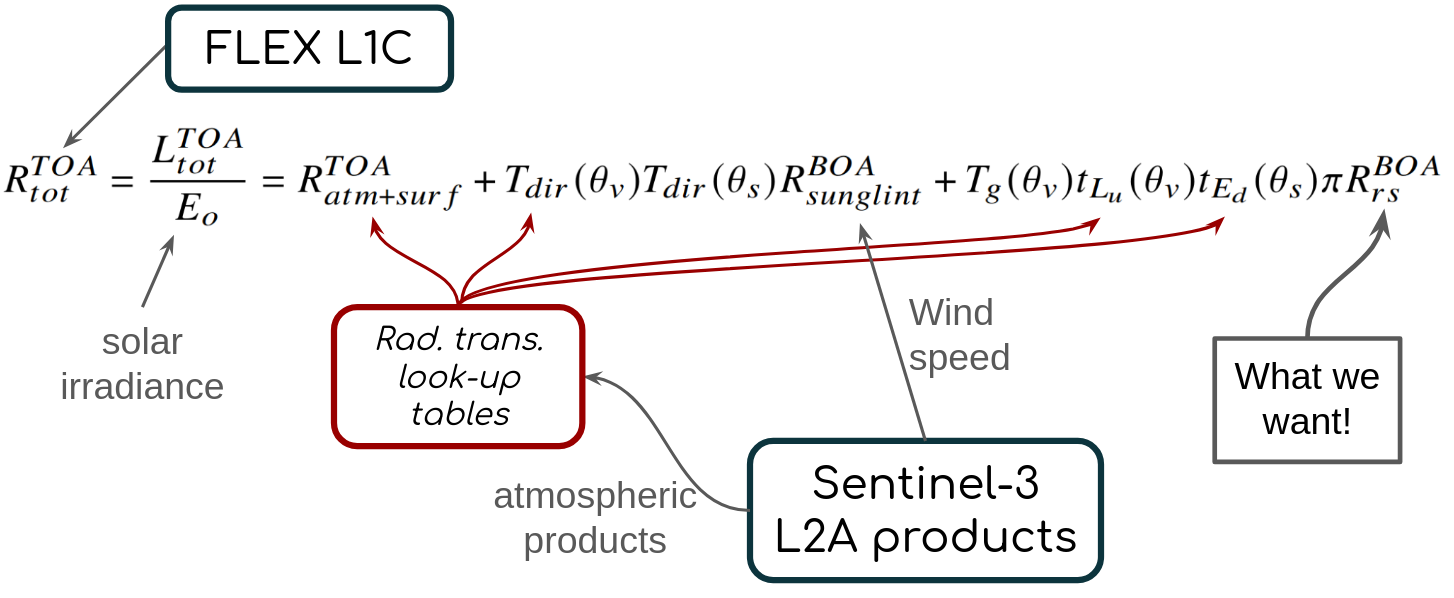
\includegraphics[width=1\linewidth]{FLEX_AC_scheme.png}
    \caption{Scheme of the synergistic approach for atmospheric correction of FLEX pixels from Sentinel-3C L2B atmospheric products (e.g., aerosol optical thickness, Angström exponent, absorbing gases, wind speed).}
    \label{fig:ac_overview}
\end{figure}


\subsection{Performance report: application to Sentinel-3 FLEX mode images}\label{sec:performance}
\subsubsection{Satellite images: Sentinel-3 FLEX mode and co-registration}
To evaluate the performance of the proposed synergistic atmospheric correction, the Sentinel-3 OLCI FLEX mode acquisitions were exploited. The first step consisted of stacking the 45 spectral bands of the S3-FLEX-mode images (ranging from 500 to 800 nm) and saving the final image in ZARR format, see Figure \ref{fig:s3flex_stacking}. Then, based on these stacked images the L2A product of Sentinel-3A, orbiting in tandem, were coregistered by bilinear spatial interpolation to the grid of S3-FLEX-mode images, see Figure \ref{fig:s3_rgb_l2a}. 

\begin{figure}[H]
    \centering
    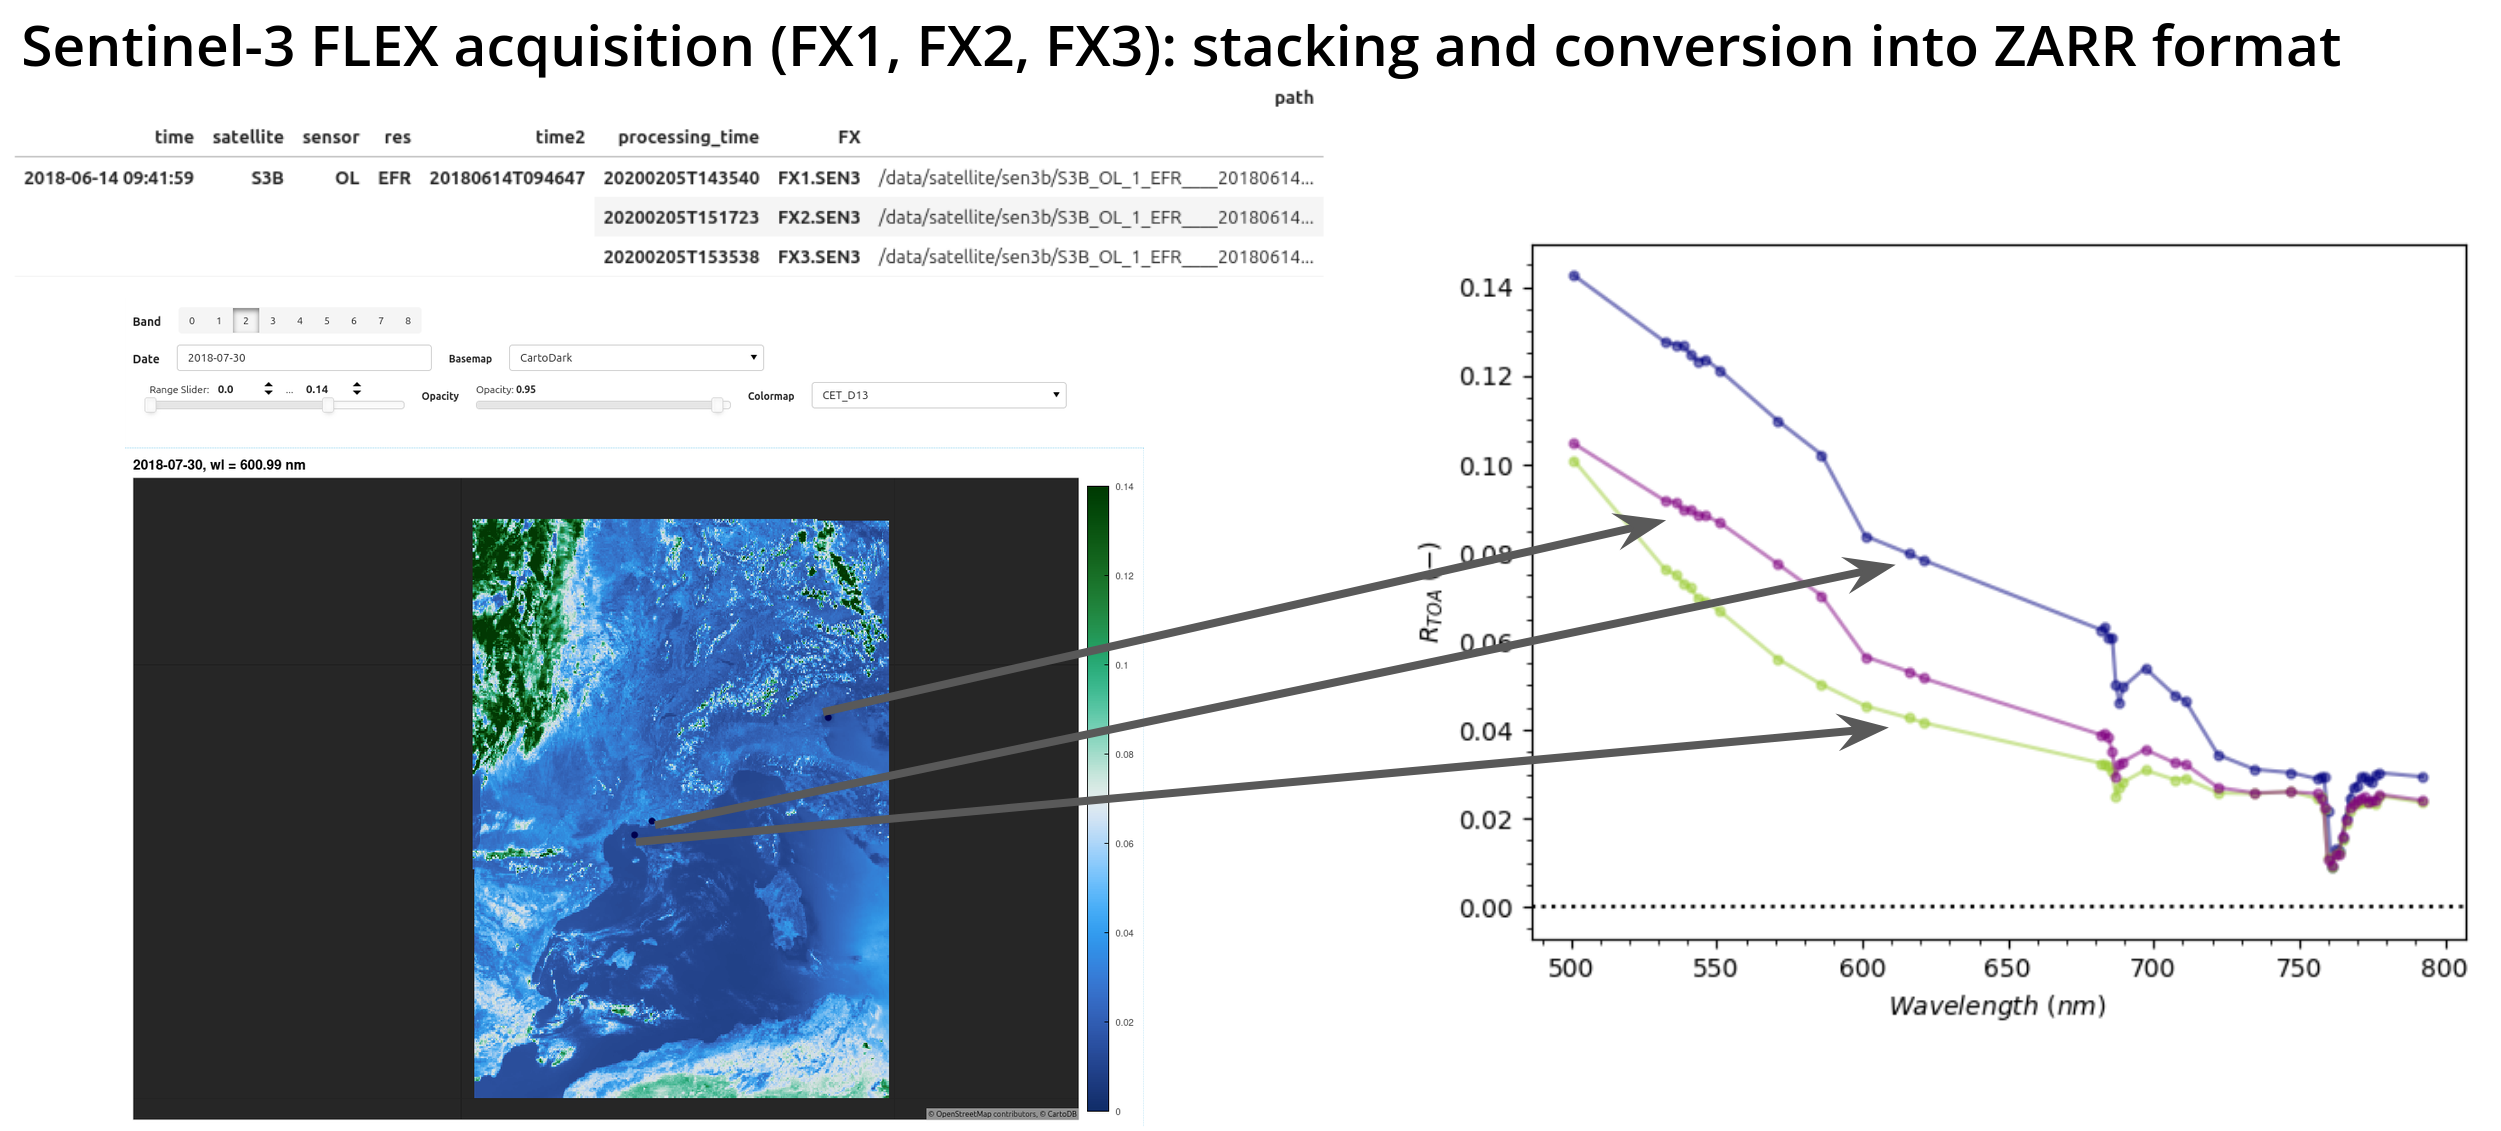
\includegraphics[width=1\linewidth]{s3_flex_mode_stacked.png}
    \caption{Stacking of the 45 spectral bands of the Sentinel-3B-FLEX-mode files (three files FX1, FX2, FX3 per acqisition) into one ZARR image enabling visualization and further processing of the L1C data.}
    \label{fig:s3flex_stacking}
\end{figure}

\begin{figure}[H]
    \centering
    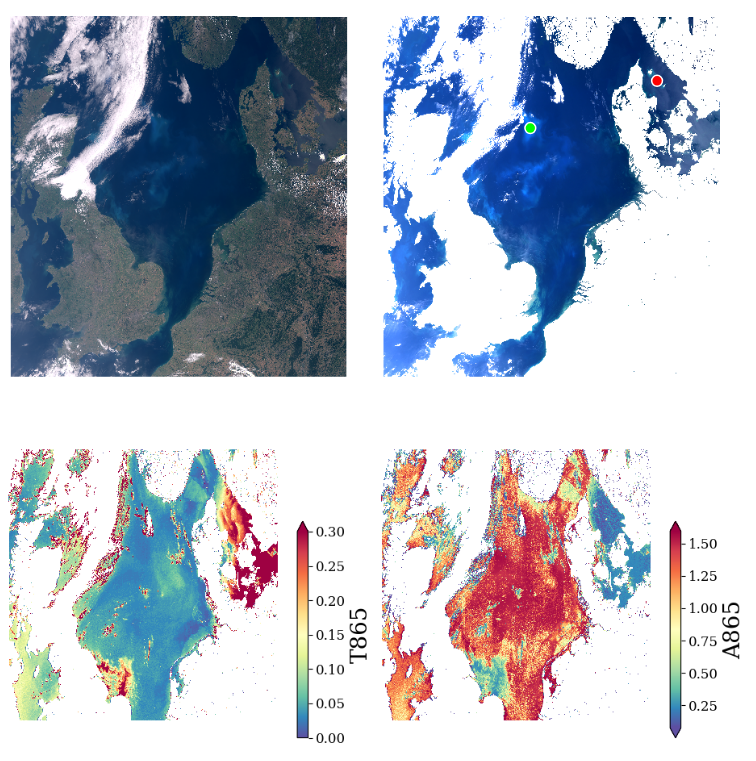
\includegraphics[width=0.75\linewidth]{s3_flex_rgb_l2a.png}
    \caption{Co-registered Sentinel-3B-FLEX-mode L1C (top row) and Sentinel-3A L2A products (bottom row showing aerosol products). (top-right panel) RGB L1C image after water masking showing a pixel in a coccolithophores bloom (green dot) and a pixel impacted by sunglint (red dot).}
    \label{fig:s3_rgb_l2a}
\end{figure}

\subsubsection{Basic pixel processing}
The full atmospheric correction procedure was applied to several L1C/L2A synergistic images. Here, we illustrate typical results for a given pixel located in a probable coccolithophore bloom (see green dor in Figure \ref{fig:s3_rgb_l2a}). The L2A parameters were used to simulate the different radiometric terms to proceed with retrieval of $R_{rs}$. The retrieved L2A aerosol optical thickness is 0.089, as it can be seen from Figure \ref{fig:basic_pixel_hyp}, this L2A value slightly overestimates the atmospheric reflectance at TOA in the NIR ($\lambda>700nm$) in comparison to the reflectance measured by S3-FLEX-mode (black dots). It is clearly visible when convoluting the hyperspectral simulation at the S3-FLEX-mode spectral characteristics (Figure \ref{fig:basic_pixel_convolved}). To get the final FLEX-mode L2A product, the aot was decreased to 0.024, the value that cancels the mean water-leaving term of the bands beyond 770 nm (outside the O$_2$-A band) where the bloom has a negligible signal, to proceed to final atmospheric correction as shown in figure \ref{fig:FLEX_mode_L2A} for the remote sensing reflectance (Eq. \ref{eq:rrs_ac}) and downwelling irradiance parameters (PAR of 1660 $\mu mol\ photon\cdot m^{-2}\cdot s^{-1}$). In the O$_2$-A band, the retrieved $R_{rs}$ is slightly negative: the band reflectance of these absorption features is very sensitive to the spectral responses of the sensor, modeled here by Gaussian functions. The retrieved $R_{rs}$ is further analyzed in section \ref{sec:compar} against species dependent simulations. The $aot$ overestimation (even small) may induce discrepancies in the FLEX L2A retrieved products, it is then argue that the algorithm should refine the aerosol estimation based on the FLEX data itself.
\begin{figure}[H]
    \centering
    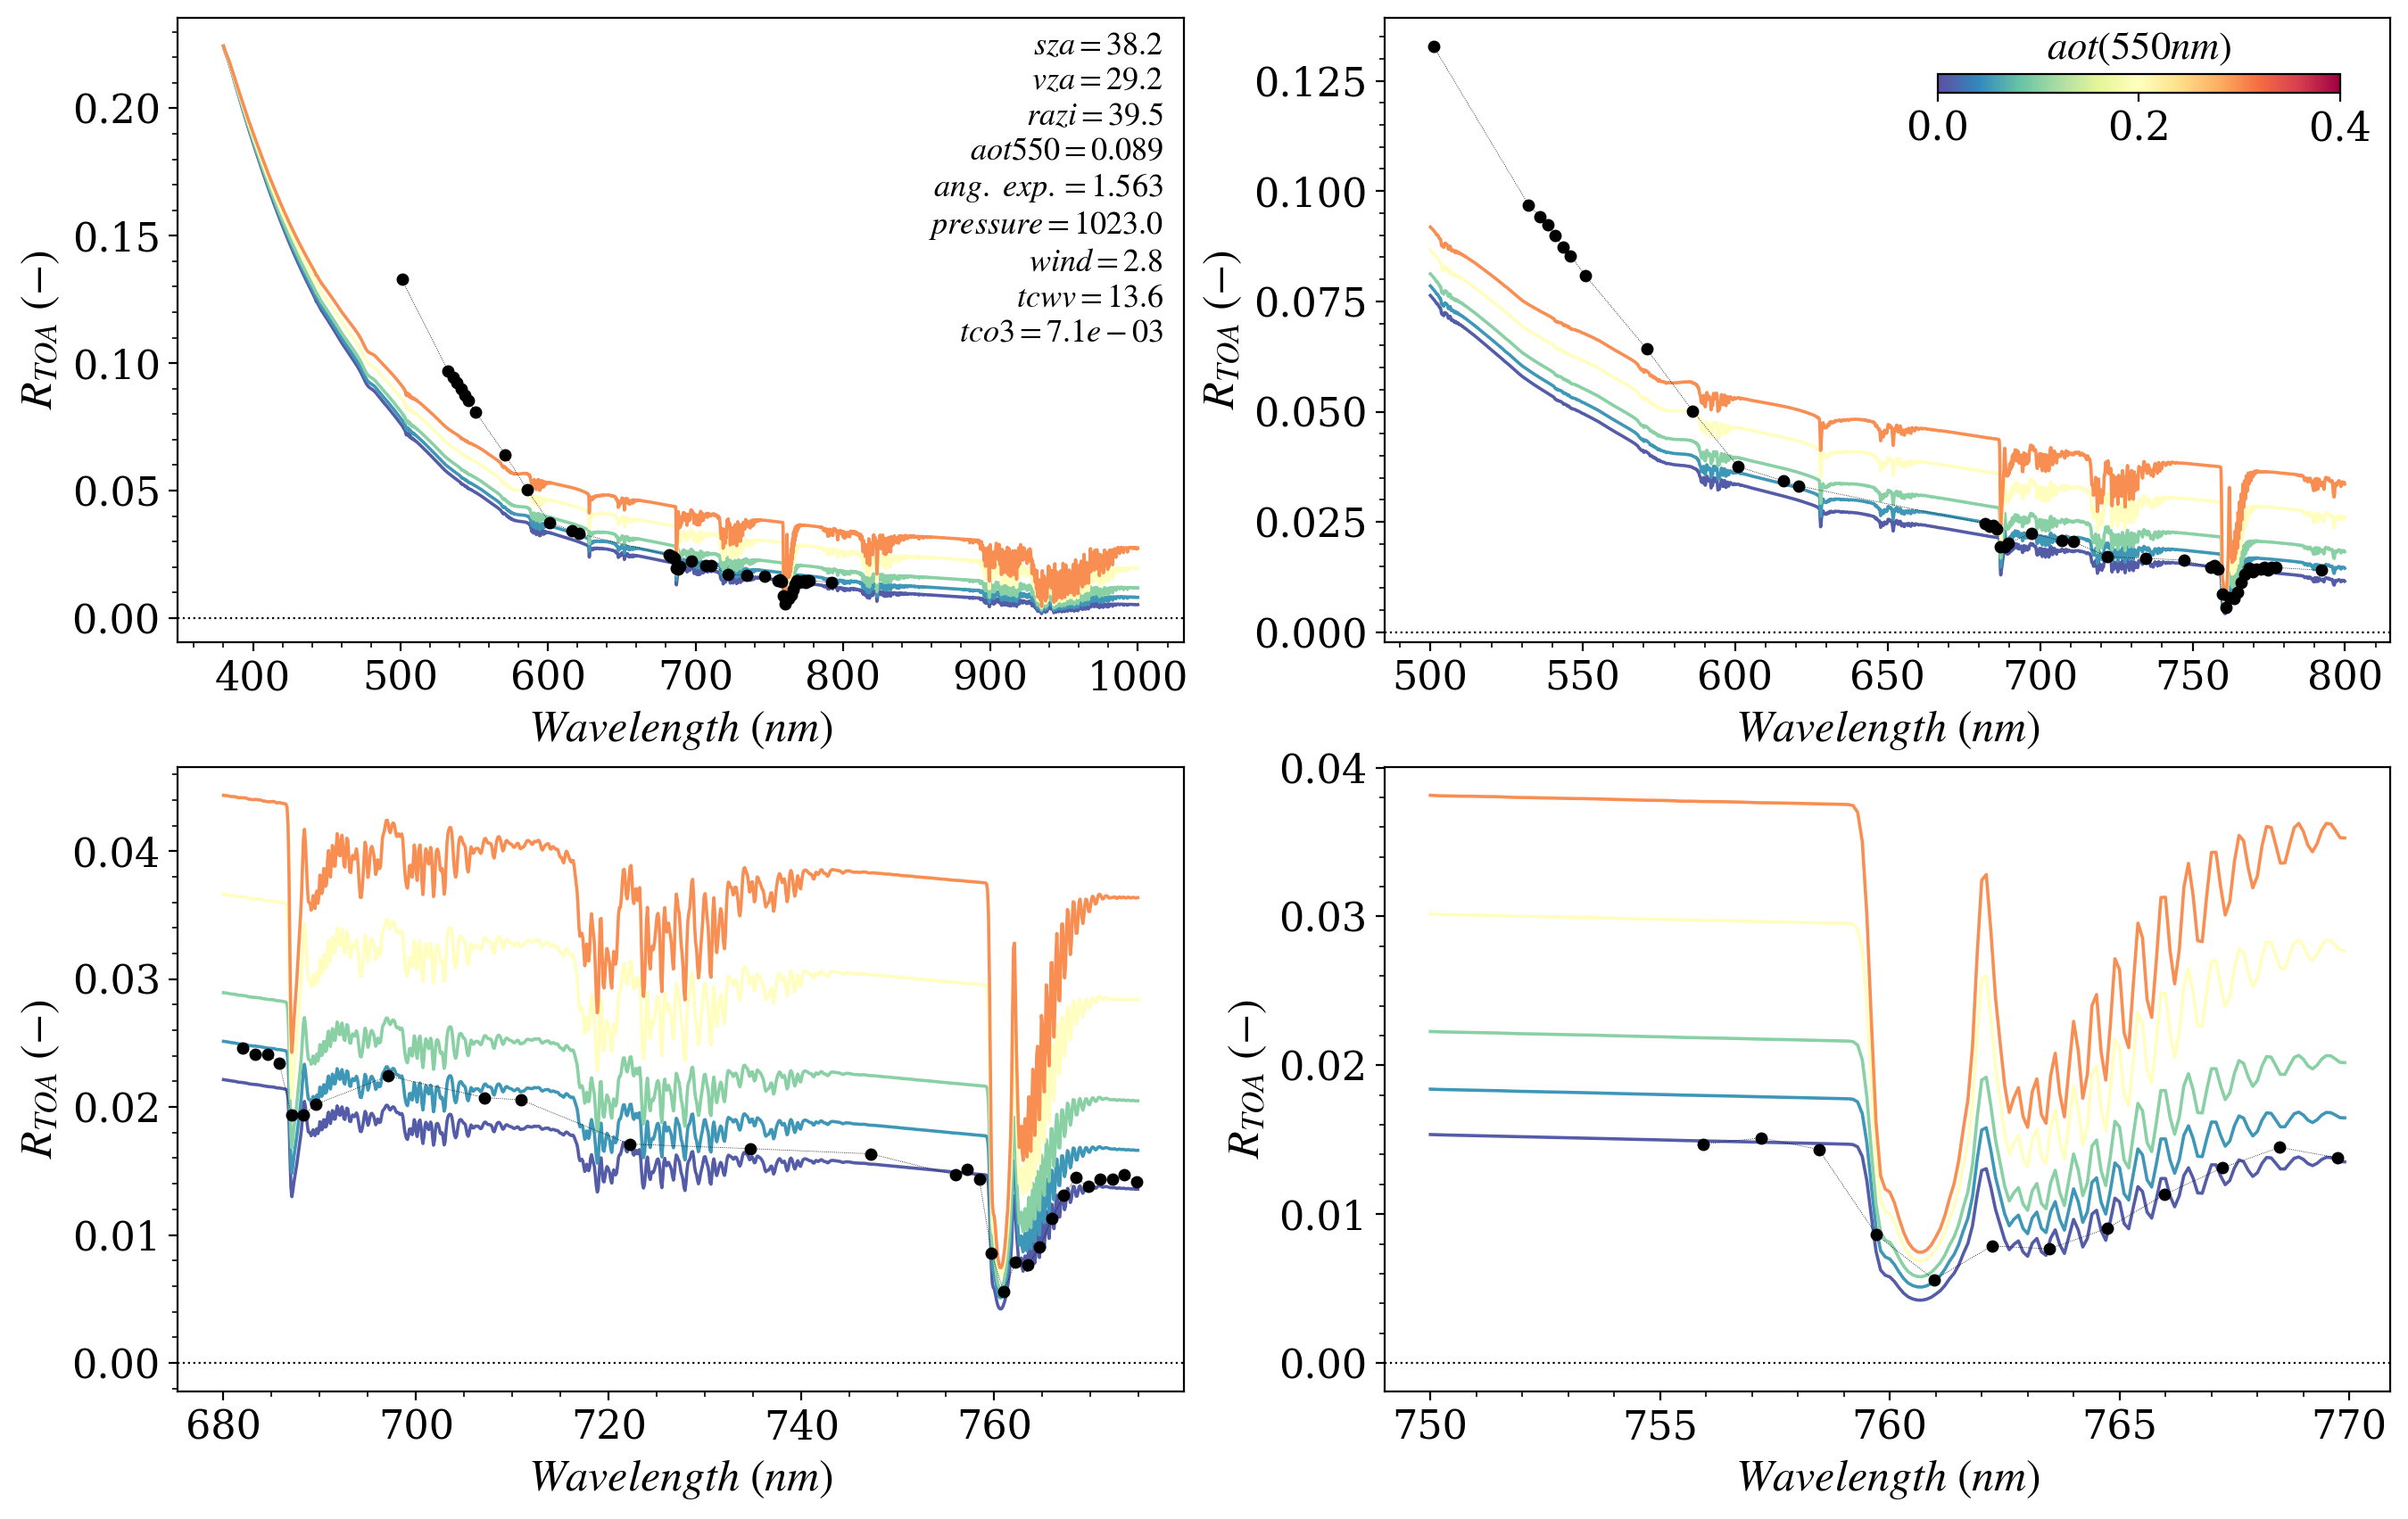
\includegraphics[width=0.85\linewidth]{basic_pixel_hyp_simu.png}
    \caption{Comparison of the top-of-atmosphere reflectance measured by S3-FLEX-mode (black dots) and simulated through the developed algorithm based on the L2A atmospheric Sentinel-3 products. Here, various aerosol optical thicknesses had been used to show the sensitivity on this input parameter.}
    \label{fig:basic_pixel_hyp}
\end{figure}

\begin{figure}[htb!]
    \centering
    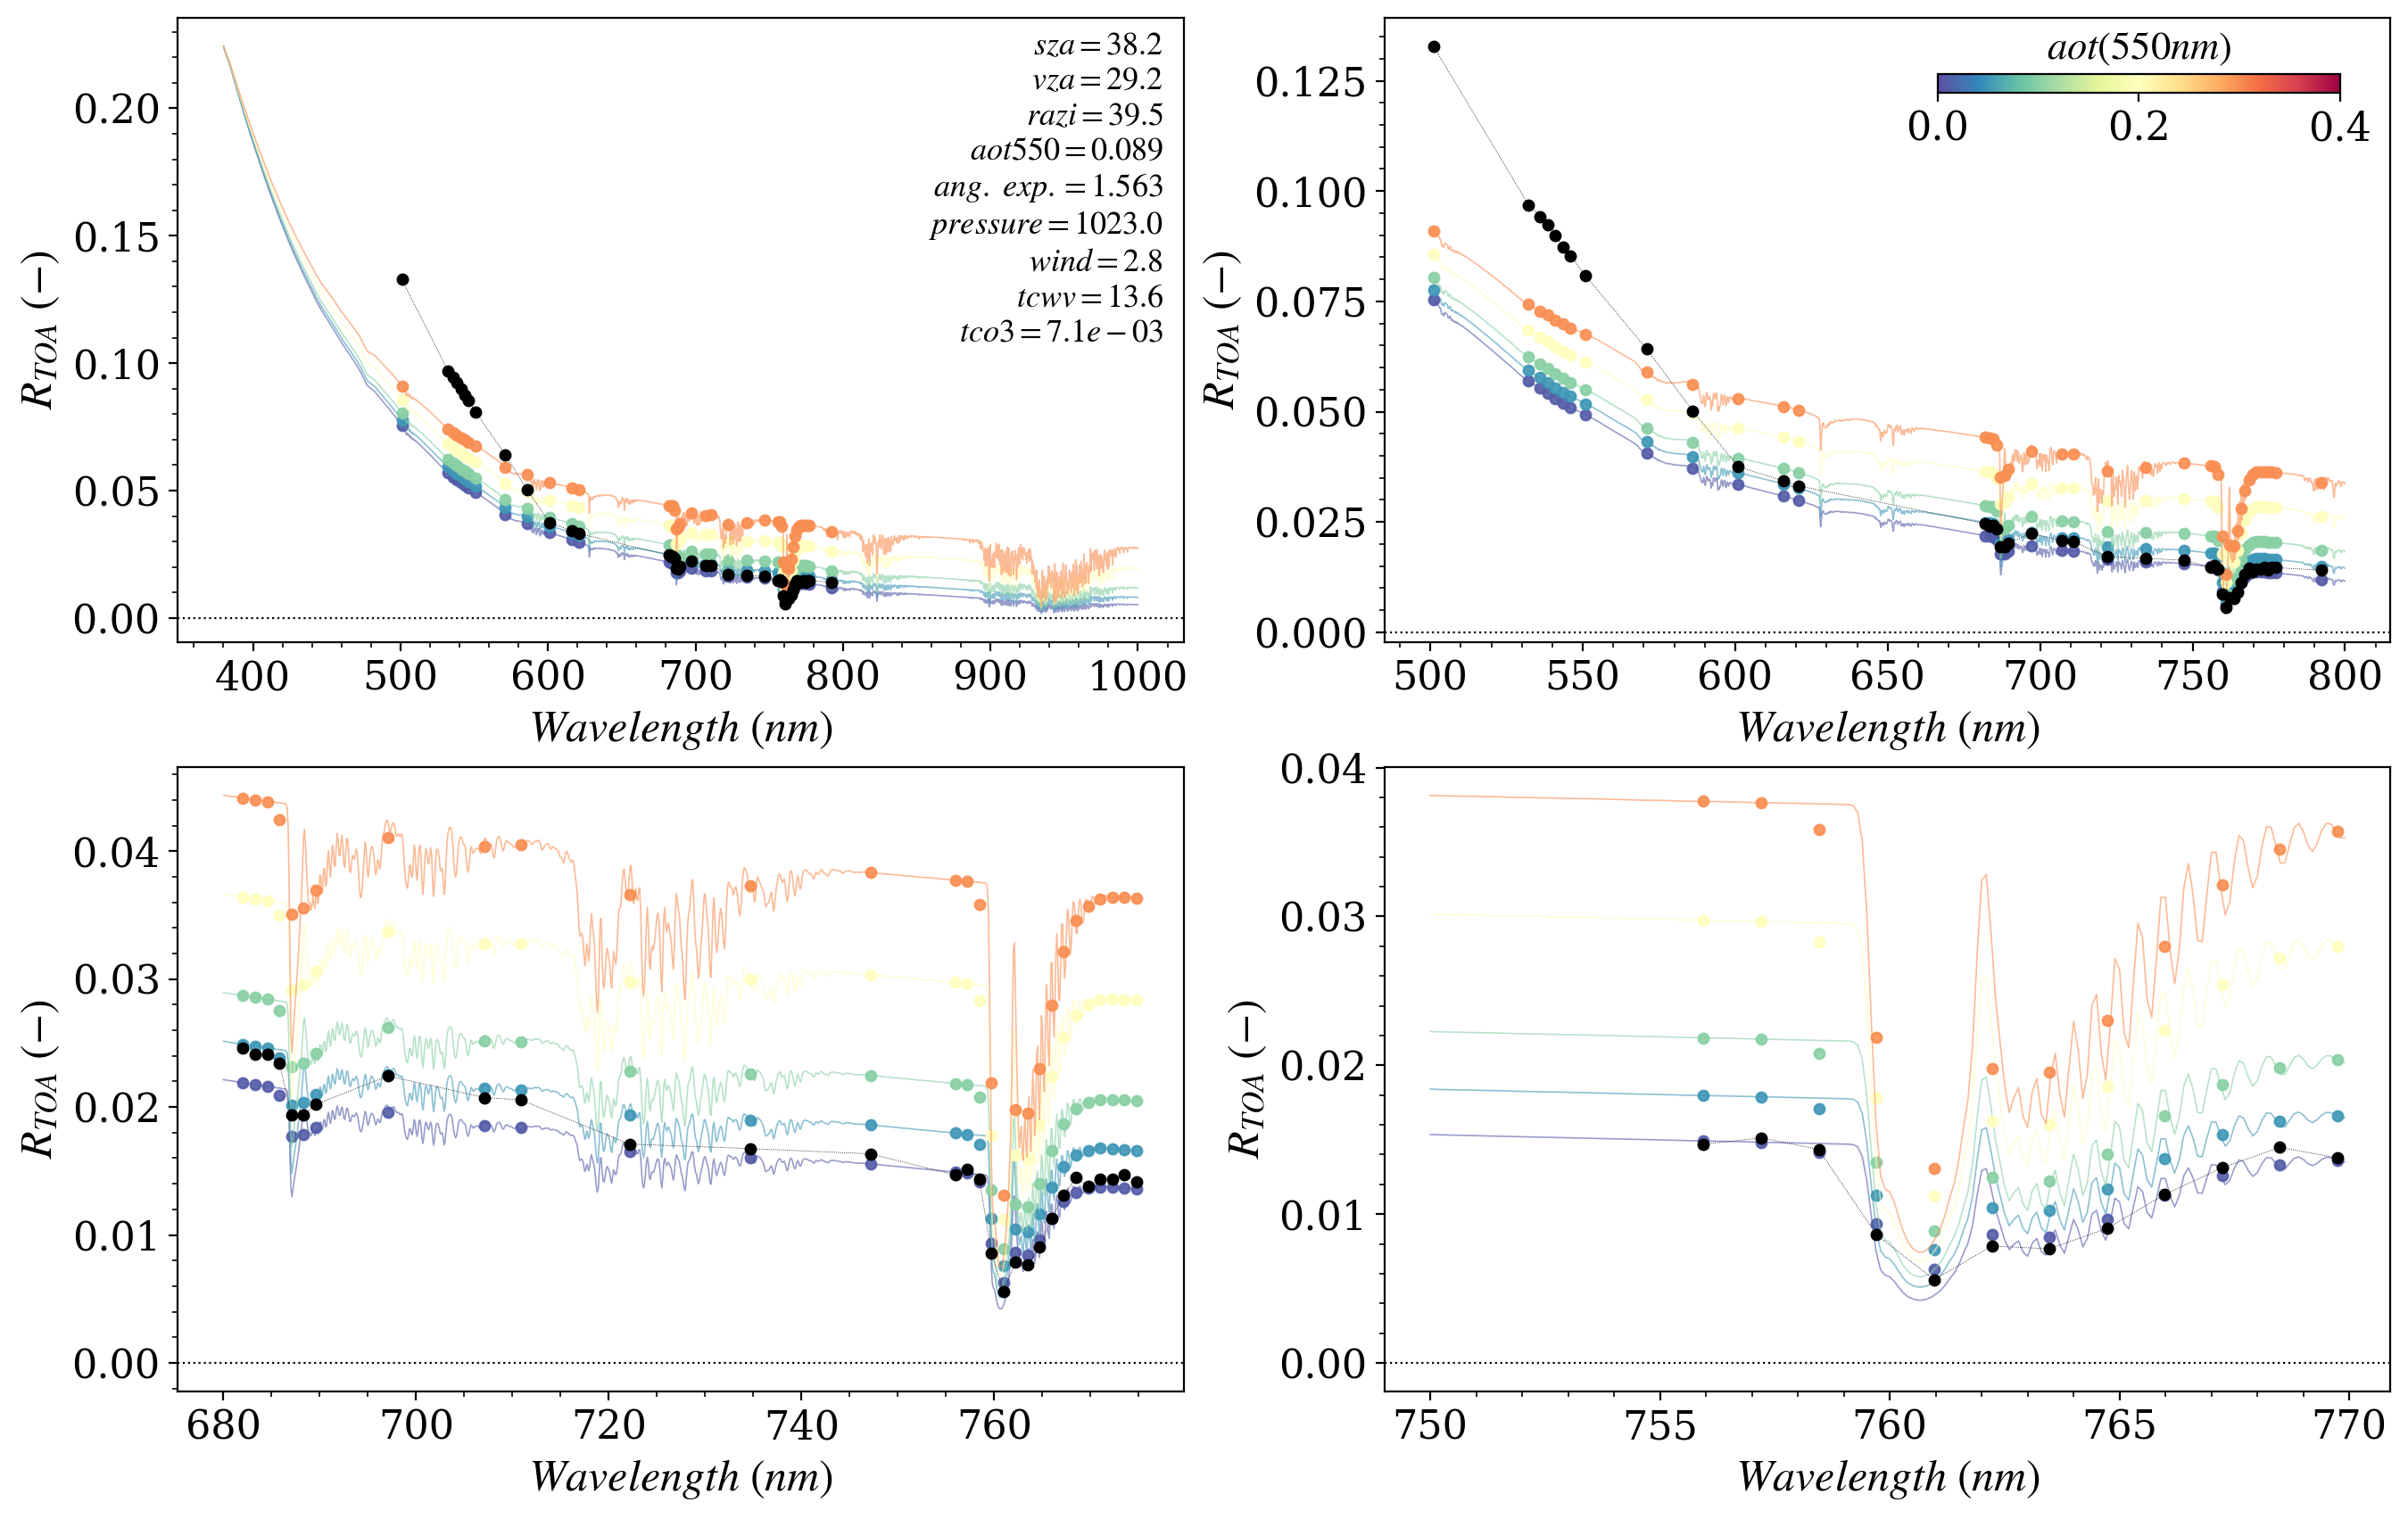
\includegraphics[width=0.85\linewidth]{basic_pixel_convolved.png}
    \caption{Similar to \ref{fig:basic_pixel_hyp} after convolution of the hyperspectral simulations with the spectral responses of the S3-FLEX-mode data.}
    \label{fig:basic_pixel_convolved}
\end{figure}

\begin{figure}
    \centering
    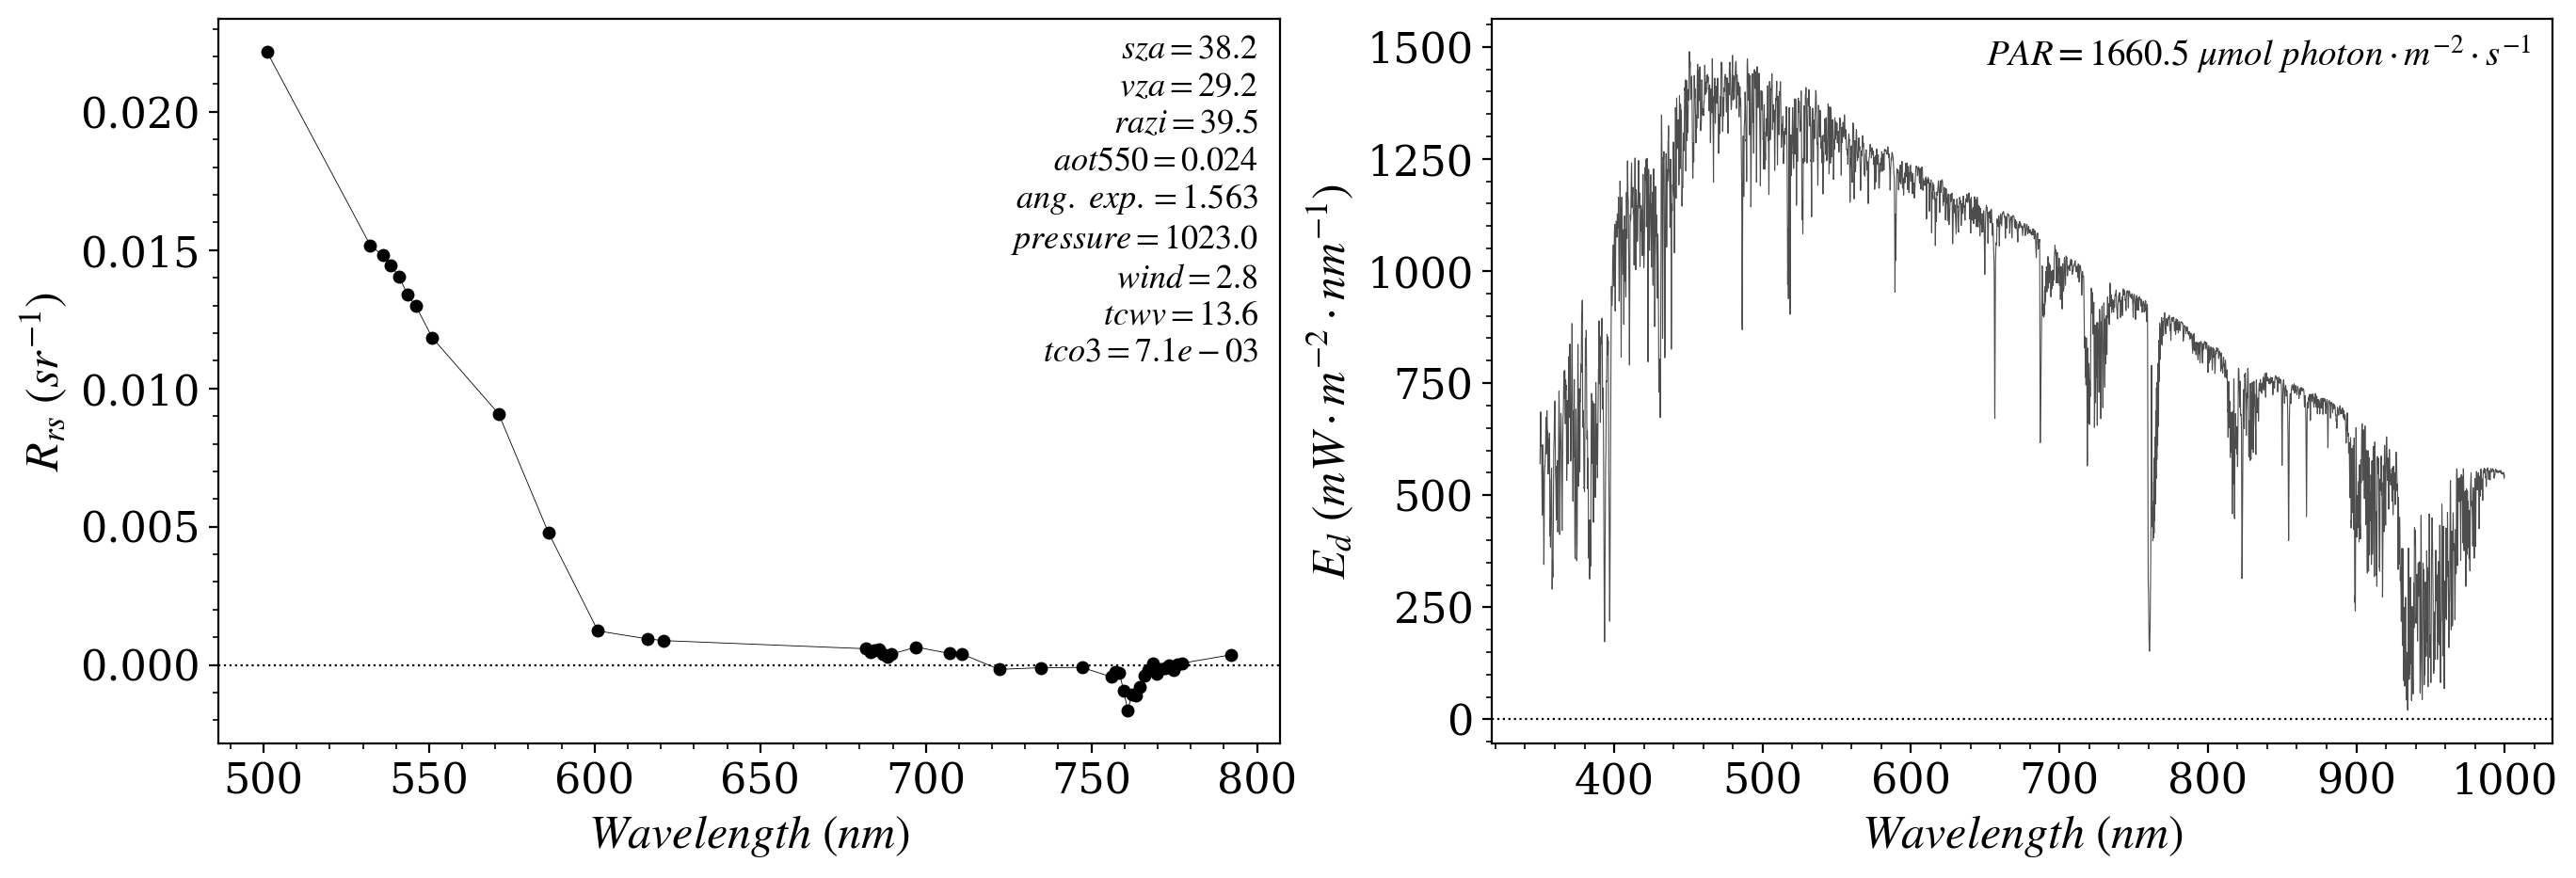
\includegraphics[width=0.9\linewidth]{basic_pixel_rrs.png}
    \caption{L2A FLEX-mode output ($R_{rs}$, $E_d$ and $PAR$) retrieved by the developed algorithm applied from the Sentinel-3A L2A atmospheric products but with a lowered value of the aerosol optical thickness (0.024)}
    \label{fig:FLEX_mode_L2A}
\end{figure}
\subsubsection{Pixel impacted by sunglint}\label{sec:sunglint_pixel}
The same procedure was applied to a Sentinel-3 FLEX-mode pixel impacted by sunglint (red dot in Fig. \ref{fig:s3_rgb_l2a}) including sunglint computation based on geometry and wind speed (here 6.2 $m\cdot s^{-1}$, isotropic Cox-Munk statistics). The L2A product indicates a high value of 0.3 for the aerosol optical thickness. However, as it can be readily seen in Fig. \ref{fig:sunglint_pixel}, the top-of-atmosphere simulation for $aot=0.3$ provides significantly higher reflectances than that measured for this pixel. In version 1.1, the L2A wind speed is used consistently for the sky reflection (LUT) and for the sunglint: the simulation then exceeds the measured reflectance beyond 770 nm for all the aerosol optical thicknesses (0.036 for $aot=0.01$ against 0.032 measured). In version 1.0, the sunglint of this figure was computed for a wind speed of 4 $m\cdot s^{-1}$, which led to $aot \approx 0.1$; with this wind speed, version 1.1 gives the same result. Both the aerosol optical thickness of the L2A product and the sunglint reflectance predicted from the L2A wind speed are therefore biased for this pixel. The overestimation of $aot$ is typical of the aerosol retrieval algorithm applied to bright sunglinted pixels. This one of the limitation of the current approach linked to potentially biased L2A products as input for the atmospheric correction. As a perspective of this work, we propose to develop and implement a second step within the algorithm to re-estimate aerosol parameters based on a non-linear approach including a specific constrain on the "non-negativity" of the retrieved $R_{rs}$ (see section \ref{sec:perspectives}).

\begin{figure}[H]
    \centering
    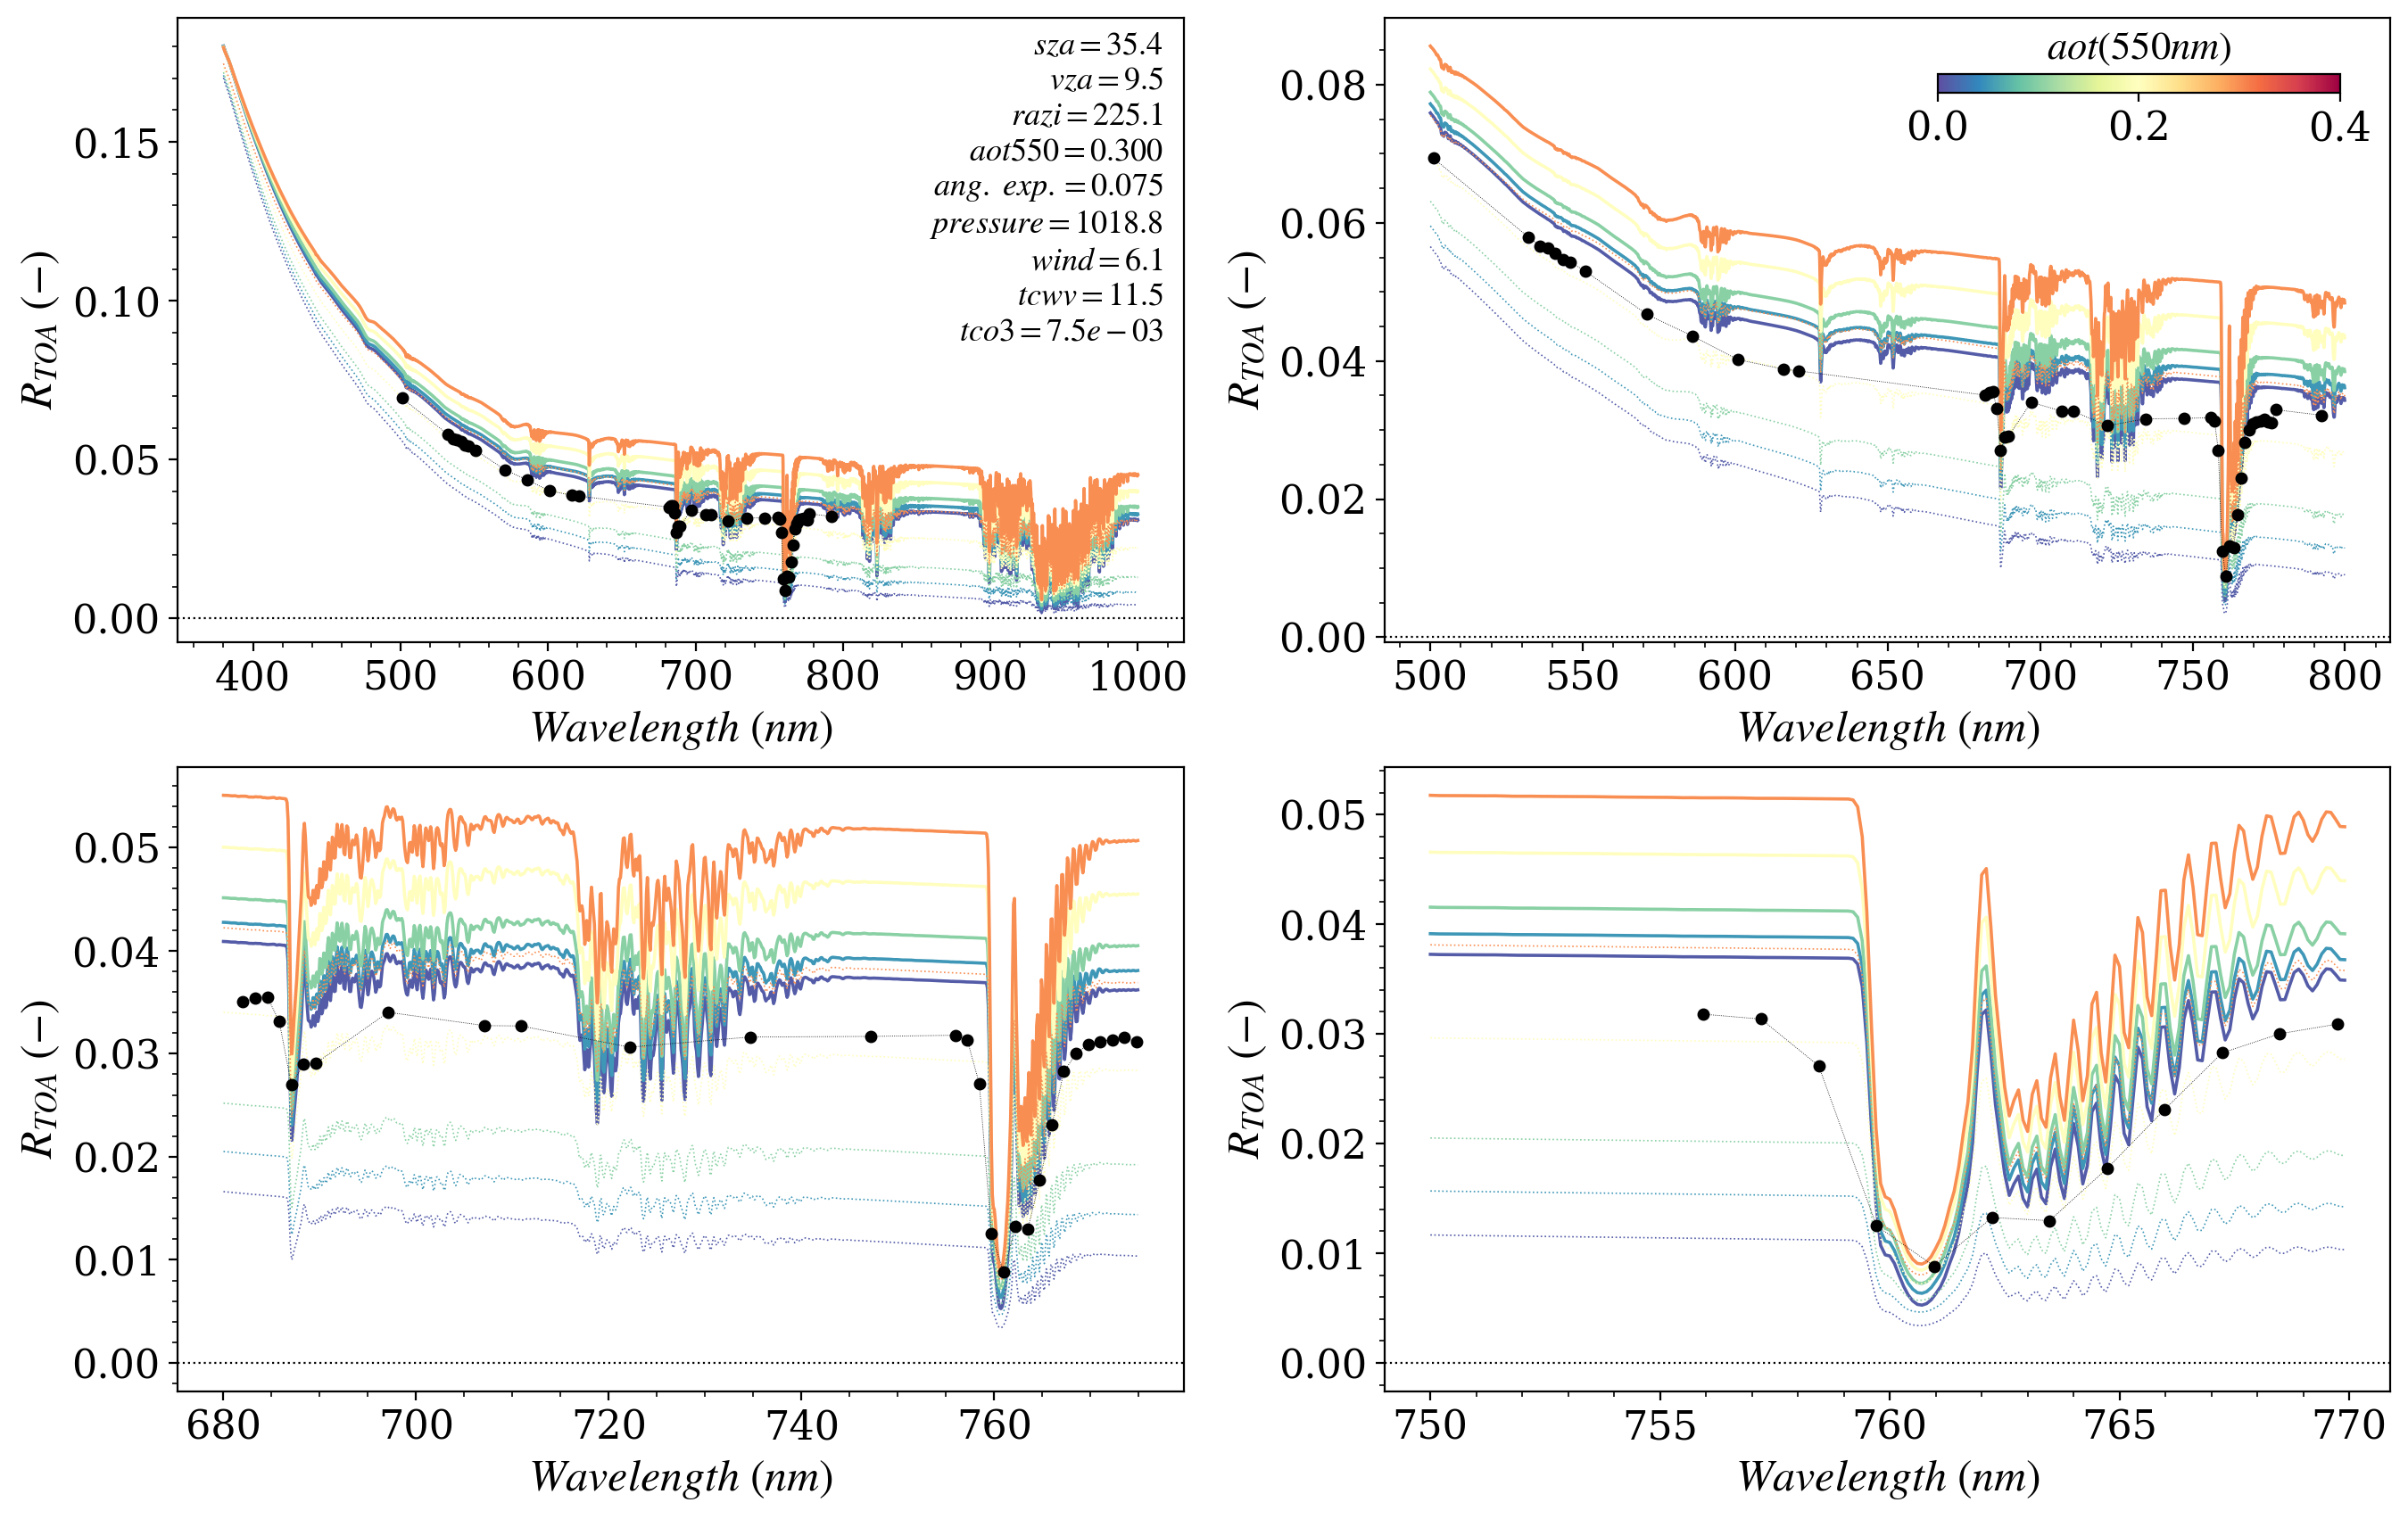
\includegraphics[width=0.9\linewidth]{sunglint_pixel_hyp_simu.png}
    \caption{Similar to Figure \ref{fig:basic_pixel_hyp} for a pixel impacted by sunglint: (dotted lines) simulated signal without sunglint, (continous lines) with addition of the sunglint contribution.}
    \label{fig:sunglint_pixel}
\end{figure}



\subsubsection{Comparison with water optics simulations}\label{sec:compar}
We provide here a comparison of the retrieved $R_{rs}$ from S3-FLEX-mode with theoretical $R_{rs}$  simulated with the package \textit{InvRrs} (Harmel, \textit{in prep.}). This comparison was made with the processing of version 1.0 ($aot=0.01$, water-leaving term at the TOA divided by $\pi$, without correction of the diffuse transmittances), and is to be updated with the $R_{rs}$ of version 1.1 (Figure \ref{fig:FLEX_mode_L2A}), larger mainly because of the correction of the diffuse transmittances. The Fig. \ref{fig:invRrs} shows the satellite data after atmospheric correction of a pixel in the middle of a bloom most likely composed of \textit{emiliania huxleyi} species in the North see (green dot in Fig. \ref{fig:s3_rgb_l2a}). Simulations were performed for the absorption coefficient of CDOM equal to 0.015 $m^{-1}$ at  440 nm, suspended particulate matter of 2 $mg\cdot m^{-3}$ and various concentration of chlorophyll-a for six different phytoplankton species. Interestingly, the only species that enables us to fit the satellite data is \textit{emiliania huxleyi} (EMI) indicated a chlorophyll-a concentration of around 0.5 $\mu g\cdot m^{-3}$.  
 \begin{figure}[H]
    \centering
    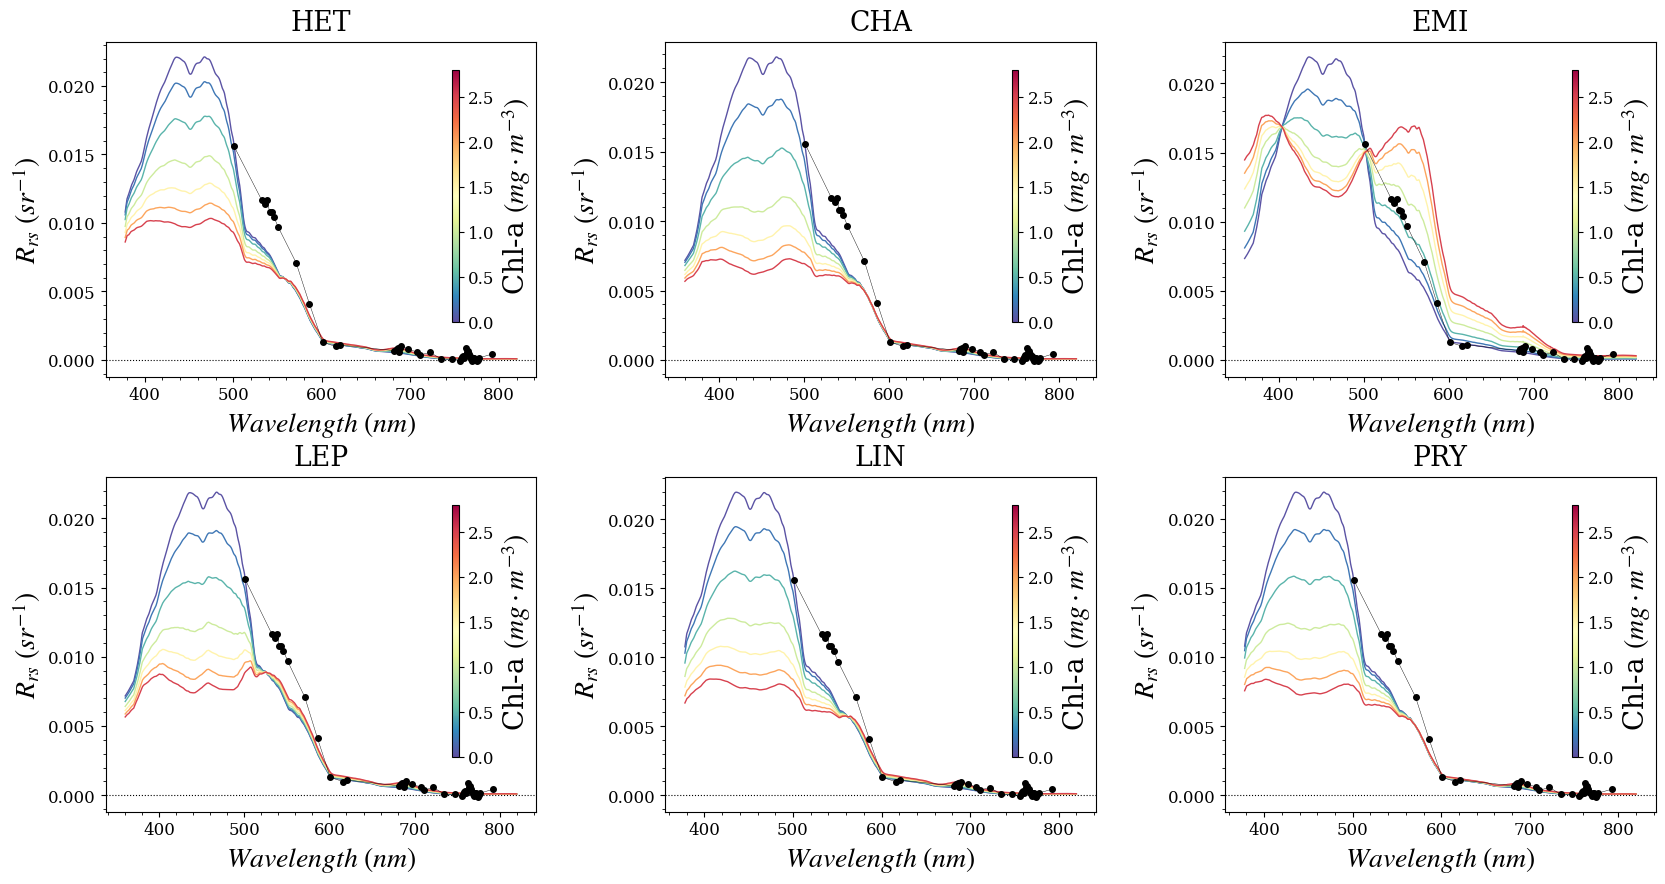
\includegraphics[width=0.95\linewidth]{Rrs_simu_basic_pixel.png}
    \caption{Comparison between retrieved $R_{rs}$ from S3-FLEX-mode data and simulations performed with invRrs package for six phytoplankton species: HET: \textit{Heterosigma akashiwo}, CHA: \textit{Chaetoceros muelleri}, EMI: \textit{Emiliania huxleyi}, LEP: \textit{Lepidodinium chlorophorum}, LIN: \textit{Lingulodinium polyedra}, PRY: \textit{Prymnesium parvum}.}
    \label{fig:invRrs}
\end{figure}


\section{Future steps: a non-linear optimization scheme}\label{sec:perspectives}
As previously discussed based on several realistic examples, the developed algorithm might fail if the L2A atmospheric parameters used as input are not accurate enough (this is especially true for region of the image impacted by sunglint). The sensitivity on the aerosol optical thickness ($aot$) parameter appeared to be critical, but we recall that the sunglint computation is directly related to the spectral values of $aot$. Thus,  improvements of the atmospheric correction are foreseen in the reajustment of the $aot$ coupled with the sunglint removal procedure. As a perspective to this work, we propose to investigate a specific algorithm procedure (\textit{hGRS}), we recently developed for atmospheric correction of PRISMA and EnMAP hyperspectral satellite images. This algorithm is based on a non-linear optimization under the constrain of non-negativity of the retrieved $R_{rs}$ to estimate the aerosol and sunglint parameters. It is here proposed to use as an input of such methods the L2A Sentinel-3 product as first guess to run the optimization. The core equation of this method could be summarized as follows. The cost function $f$ is constructed based on this formulation:
\begin{equation}
      f_{\lambda_i}(aot550,BRDFg)  = R_{mes}(\lambda_i) - R_{sim}(\lambda_i, aot550, BRDFg)
\label{eq:placeholder}
\end{equation}
with the two unknowns $\mathbf{x}={aot550, BRDF_g}$, and $R_{sim}$ the radiative transfer forward model described in this document. The optimization under constrain amounts to solve the following system:


\begin{equation}
f\left( \textbf{x} \right)\sim \sum_{wl\ \in\ SWIR}^{}\left(R^{sat}_{TOA}-R^{sim}_{TOA}\left( \textbf{x} \right)  \right)^{2} 
\label{eq:placeholder}
\end{equation}
\begin{equation}
c_{j}\left( \textbf{x} \right)=R_{rs}\left(\textbf{x} ,\lambda_{j} \right),\ j\in \left\{ 400,900 nm \right\}
\label{eq:placeholder}
\end{equation}
\begin{equation}
\textbf{x}=\left\{ aot, wv,BRDF_{g} \right\}
\label{eq:placeholder}
\end{equation}


\section{Conclusion}
A complete first scheme for atmospheric correction of FLEX was described based on synergistic use of the Sentinel-3 L2A atmospheric product and L1C FLEX images. The main equations and principles were briefly summarized in order to provide a meaningful description of the pre-computed look-up tables (LUT) and radiative transfer model used to simulate the FLEX top-of-atmosphere signal over the aquatic environment (coupled atmosphere-interface-water system). The LUT were generated using the OSOAA and LibRadTran libraries and stored in \textit{netcdf} files. As a pre-operational code, the developed algorithm applies to a single pixel to provide the remote sensing reflectance, $R_{rs}$, and the spectrally resolved downwelling irradiance at bottom-of-atmosphere with its integrated counterpart of \textit{photosynthetically active radiation} (PAR). Demonstrations were given based on the Sentinel-3 FLEX mode raster images. The next steps will be as follows:
\begin{itemize}
    \item full implementation for full raster processing,
    \item development of non-linear optimization based on the constrain of non-negativity of the retrieved $R_{rs}$, retrieving jointly the aerosol optical thickness and the sunglint (Section \ref{sec:sunglint_pixel}),
    \item validation of the coupled gaseous transmittances in the O$_2$ and H$_2$O bands with the actual spectral responses of FLEX.
\end{itemize}
Since version 1.1, the coupling between gaseous absorption and scattering within the atmosphere is accounted for, based on the
SOS-ABS code (\textit{Successive Orders of Scattering method coupled with the gaseous ABSorptions}), see
\url{https://github.com/CNES/RadiativeTransferCode-SOS}, as well as the line-by-line absorption of O$_2$ (Sections
\ref{sec:o2_lbl} and \ref{sec:coupling}).



\clearpage
\addcontentsline{toc}{section}{References}
\bibliographystyle{apalike}
\bibliography{references}

\end{document}
